\begin{apendicesenv}

% \partanexos

\chapter{Personas}
\label{personas}

\section{Persona 1}

\textbf{Perfil e Fatos Concretos}

Carlos Eduardo é um estudante universitário de 25 anos. Ele mora com a família em um pequeno apartamento no Gama, Distrito Federal. Além da universidade, também é estagiário de uma pequena empresa da região, o que deixa sua rotina com pouco tempo livre. 

\textbf{Comportamento e Hábitos}

Carlos é uma pessoa muito esforçada e que se empenha no que faz. Entretanto, seu déficit de atenção, impaciência e uma ocasional procrastinação são obstáculos que o atrapalham, principalmente nos estudos. Para relaxar, ele gosta de jogar videogame, passar tempo com os amigos e fazer caminhada ao ar livre. Também gosta de ver vídeos curtos e usar redes sociais, como Instagram e Facebook. Possui forte interesse em atividades artísticas, possuindo o objetivo pessoal de aprender a tocar violão.

\textbf{Objetivos e Necessidades}

\begin{itemize}
\item \textbf{Objetivo Principal}: Aprender a tocar violão de forma consistente e com progresso visível.

\item \textbf{Necessidades}:

\begin{itemize}

\item \textbf{Acompanhamento Personalizado}: Precisa de alguém que possa dar \textit{feedback} direto e corrigir erros práticos (como a posição das mãos ao tocar o
violão).

\item \textbf{Flexibilidade de Horários}: Por ter uma agenda muito ocupada, precisa que suas aulam possam ser marcadas em horários específicos, geralmente à noite.

\item \textbf{Indicação de Confiança}: Precisa de uma fonte confiável para encontrar um professor confiável e competente, pois não possui indicações de amigos ou familiares.

\end{itemize}

\end{itemize}

\textbf{Frustrações}

Carlos se frustra muito com a falta de interação humana durante seu aprendizado de violão. No pouco tempo livre que possui à noite, ele tenta se dedicar ao \textit{hobby} através de cursos e vídeos online, mas não sente que está progredindo, se sentindo paralisado por dúvidas simples que os materiais gravados não conseguem sanar, como o posicionamento correto das mãos no instrumento musical.

Ele sente falta de ter alguém para tirar dúvidas pontuais e receber orientação personalizada, mas não conhece pessoalmente ninguém que possa ensiná-lo e não tem indicações de escolas de música ou tutores particulares em sua região.

\textbf{Familiaridade com Tecnologia}

Carlos é capaz de utilizar seu celular e computador diariamente sem nenhum problema. Está acostumado a usar redes sociais para comunicação e consome conteúdo em plataformas de vídeo. Além disso, está acostumado a usar plataformas de videochamada, como Google Meets e Microsoft Teams, visto que as usa frequentemente para realizar trabalhos da faculdade, sentindo-se confortável com interações e reuniões em ambiente online.

\newpage

\section{Persona 2}

\textbf{Perfil e Fatos Concretos}

Ricardo Almeida tem 38 anos, é casado e professor de música na Escola de Música de Brasília. Apaixonado por sua profissão, ele encontra grande satisfação em lecionar. Para complementar o orçamento da família,  ele oferece aulas particulares de violão e de guitarra durante a noite e fins de semana.

\textbf{Comportamento e Hábitos}

Como professor, Ricardo é muito paciente, didático e dedicado. Ele acredita que qualquer pessoa pode aprender música com o método e o incentivo certos, ficando muito feliz ao ver o progresso de seus alunos. Embora seja excelente em ensinar, Ricardo possui muita dificuldade em se promover com marketing digital nas redes sociais.

\textbf{Objetivos e Necessidades}

\begin{itemize}
\item \textbf{Objetivo Principal}: Aumentar sua base de alunos particulares para aumentar sua renda mensal e ter mais segurança financeira.

\item \textbf{Necessidades}:

\begin{itemize}

\item \textbf{Maior Visibilidade}: Precisa de uma forma de alcançar pessoas que estão procurando por aulas de música, em vez de tentar a sorte com o público geral das redes sociais.

\item \textbf{Ser Recomendado}: Deseja um espaço para construir uma reputação sólida baseada em sua experiência e nas avaliações de alunos, algo que pareça mais convincente que um perfil de Instagram.

\item \textbf{Gestão Simplificada}: Necessita de uma ferramenta para organizar seus horários e agendamentos de forma simples, sem depender de inúmeras trocas de mensagens pelo WhatsApp.

\end{itemize}

\end{itemize}

\textbf{Frustrações}

A principal frustração de Ricardo é a dificuldade em encontrar novos alunos. Atualmente, sua única forma de divulgação é um perfil no Instagram, onde ele posta vídeos tocando instrumentos musicais oferecendo dicas. Entretanto, se sente desmotivado com o baixo alcance de suas publicações, percebendo que a rede social promove perfis de entretenimento e grandes influenciadores, enquanto seu conteúdo, mais técnico e didático, raramente chega a potenciais clientes.

Ele sabe que é um bom professor, mas sente que não consegue a visibilidade que precisa para conseguir novos aprendizes. Além da dificuldade de divulgação, o processo de agendamento é manual e caótico, dependendo de conversas no WhatsApp que muitas vezes se estendem por dias e não resultam em uma aula de fato.

\textbf{Familiaridade com Tecnologia}

Ricardo é familiarizado com aplicativos e redes sociais, usando constantemente o WhatsApp e o Instagram para comunicação. Utiliza o Zoom e Google Meets para realizar suas aulas online. Sua dificuldade não está em usar essas ferramentas, mas em utilizá-las para marketing e obtenção de novos clientes de forma eficaz.

\chapter{Simulação da Arquitetura}
\label{simulacao}

Com o objetivo de verificação da viabilidade da arquitetura proposta na Seção \ref{arquitetura}, foi realizada uma simulação envolvendo alguns casos de uso da proposta do software. Nesta simulação foram realizadas as conexões entre o \textit{backend}, \textit{frontend} e o banco de dados, bem como a geração das imagens Docker e orquestração com Docker Compose.

A simulação consistiu em satisfazer parcialmente as histórias de usuário US01 (\textit{Login}), US07 (Solicitar Horário) e US16 (Conquistas).

A Figura \ref{fig:login} apresenta a interface de usuário para a ação do \textit{login}, em que é possível ver os campos destinados para o preenchimento de e-mail e senha para autenticação. Caso haja falha na autenticação, é exibida uma mensagem de erro para o usuário, advinda do \textit{backend} e tratada no \textit{frontend}, conforme apresentado na Figura \ref{fig:login-erro}.

\begin{figure}[h!]
    \centering
    \caption{Interface de \textit{login}.} 
    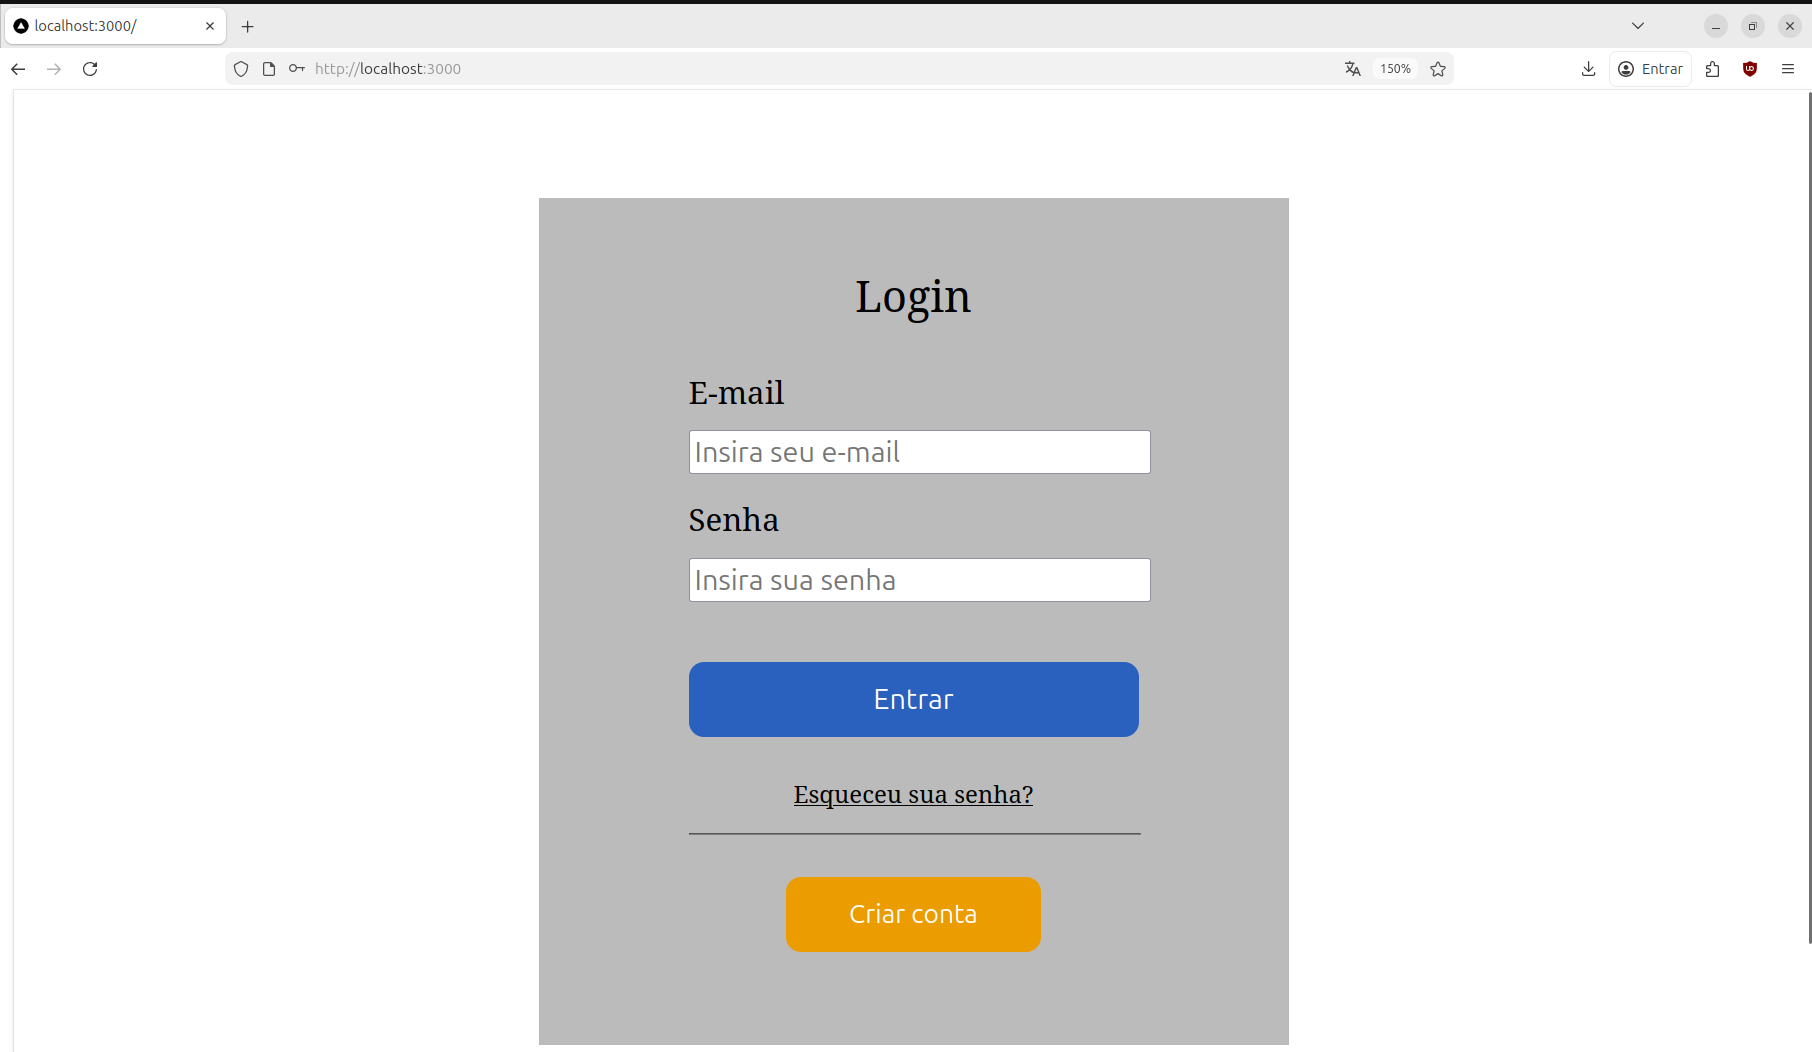
\includegraphics[width=0.99\textwidth]{figuras/login.png}
    
    Fonte: Autoria própria.
    
    \vspace{0.2cm}
        
    \label{fig:login}
\end{figure}

\begin{figure}[h!]
    \centering
    \caption{Mensagem de erro de autenticacação.} 
    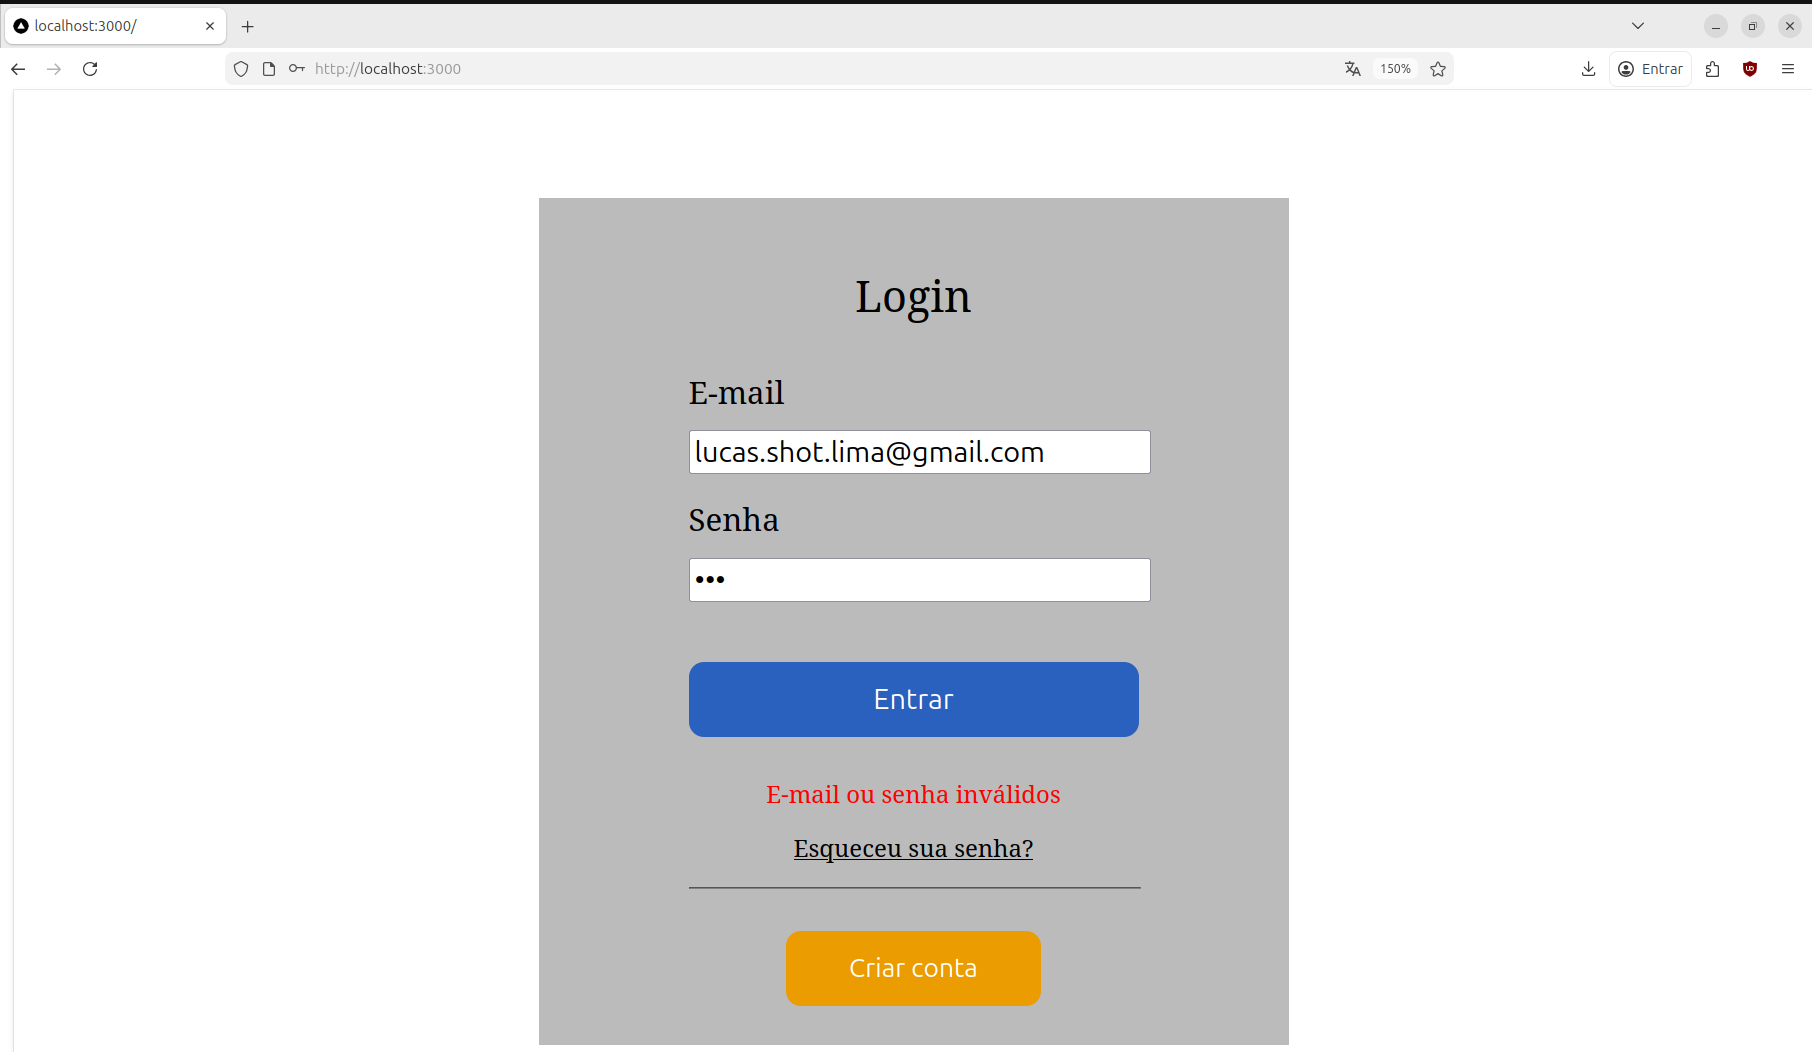
\includegraphics[width=0.99\textwidth]{figuras/login-erro.png}


    Fonte: Autoria própria.
    
    \vspace{0.2cm}
        
    \label{fig:login-erro}
\end{figure}

\newpage

A Figura \ref{fig:conquistas-bloqueadas} apresenta a tela de conquistas, a qual mostra a lista de conquistas com título, descrição, imagem e a pontuação fornecida ao usuário caso ele a desbloqueie. Conquistas bloqueadas são apresentadas com foto e texto em tom de cinza.

\begin{figure}[h!]
    \centering
    \caption{Lista de conquistas.} 
    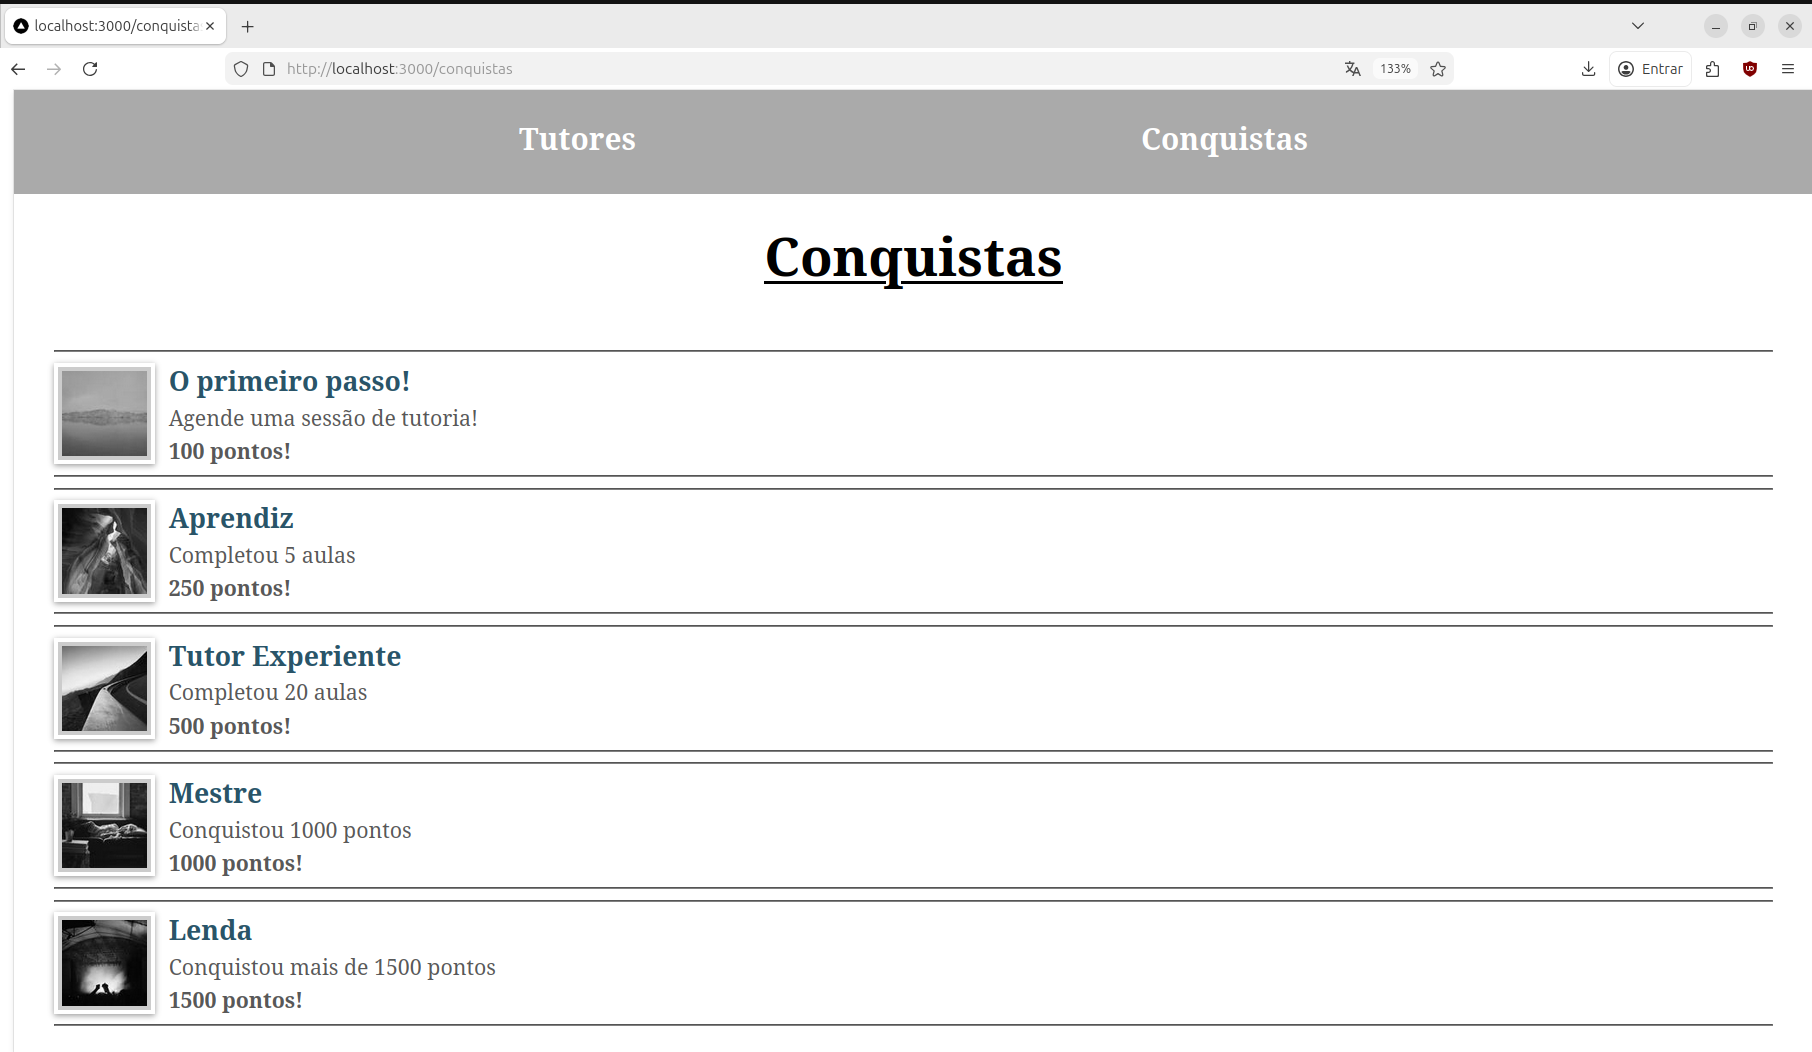
\includegraphics[width=0.99\textwidth]{figuras/conquistas-bloqueadas.png}


    Fonte: Autoria própria.
    
    \vspace{0.2cm}
        
    \label{fig:conquistas-bloqueadas}
\end{figure}

A Figura \ref{fig:tutores} apresenta a tela de tutores, que exibe tutores e suas informações, como nome, foto e áreas de conhecimento, além de dois botões interativos para o aprendiz acessar o perfil do tutor e também para solicitar uma sessão de tutoria.

\begin{figure}[h!]
    \centering
    \caption{Lista de tutores.} 
    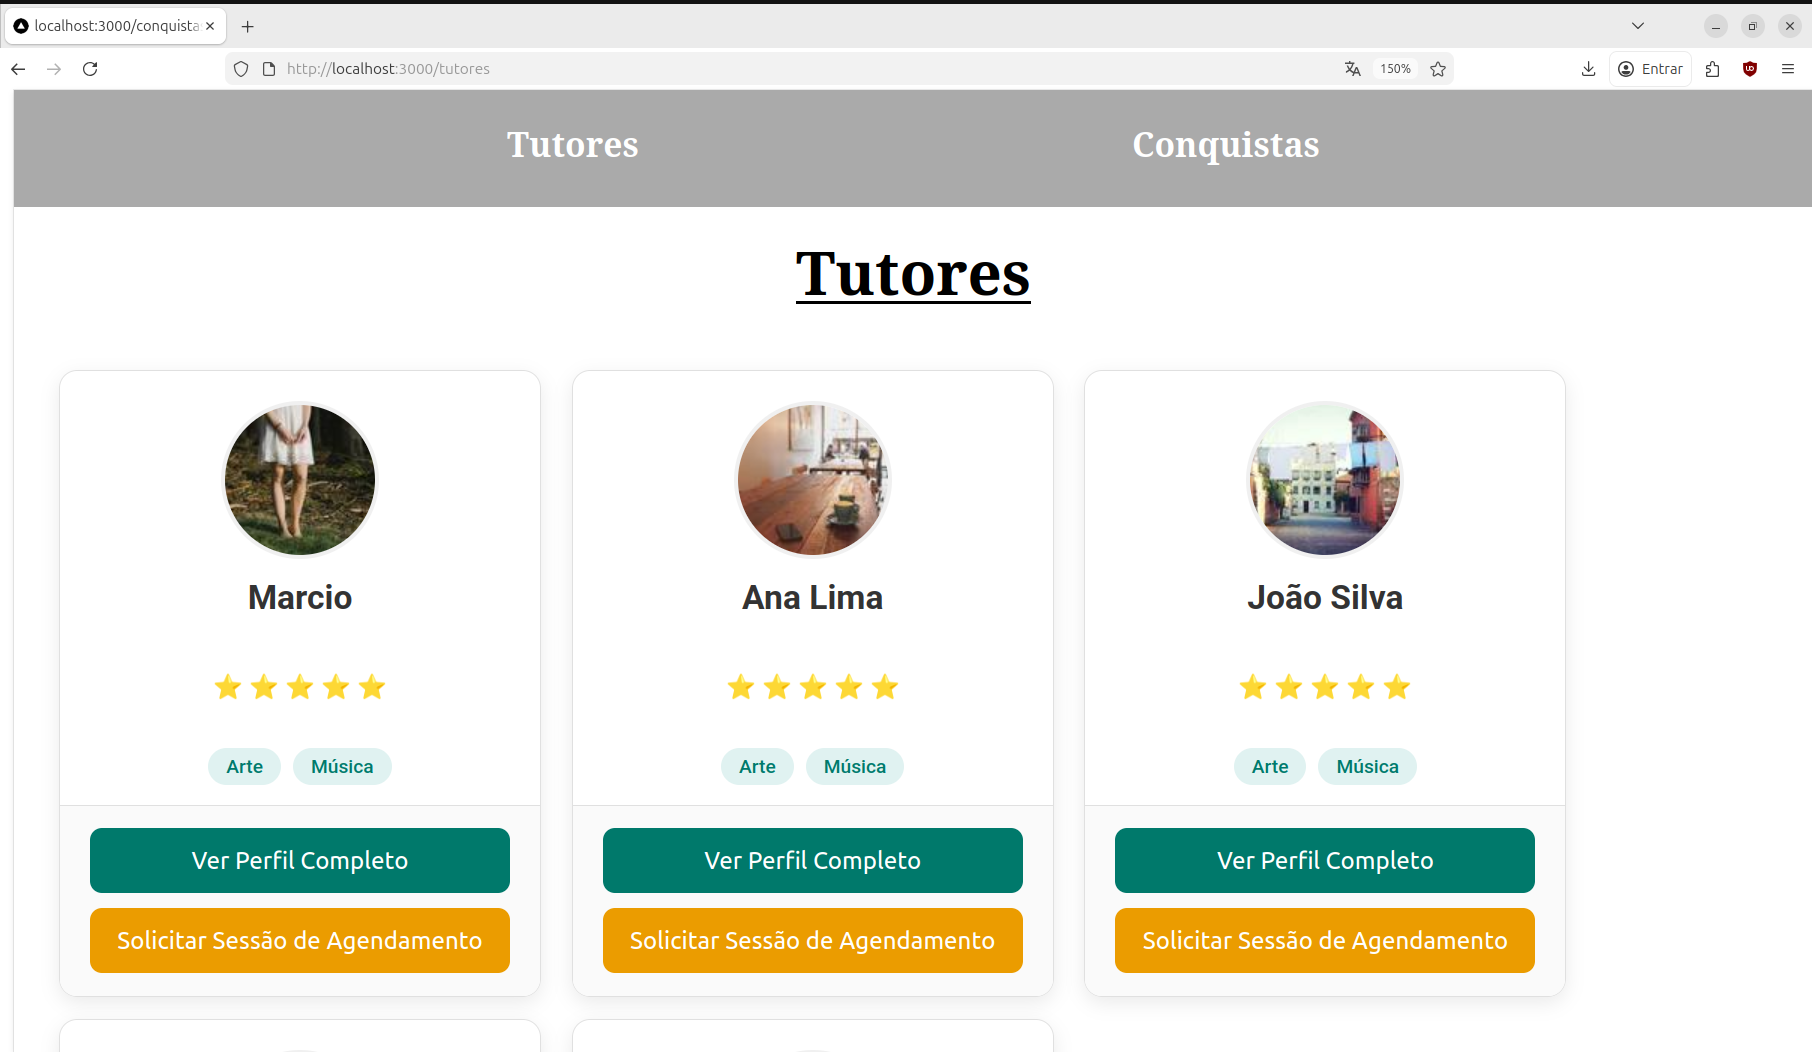
\includegraphics[width=0.99\textwidth]{figuras/tela-tutores.png}


    Fonte: Autoria própria.
    
    \vspace{0.2cm}
        
    \label{fig:tutores}
\end{figure}

Ao clicar no botão para solicitar uma sessão, abre-se uma janela em que são exibidos os horários disponíveis na agenda do tutor, conforme aprensentado pela Figura \ref{fig:sessoes}.

\newpage

\begin{figure}[h!]
    \centering
    \caption{Interface de agendamento da sessão de tutoria.} 
    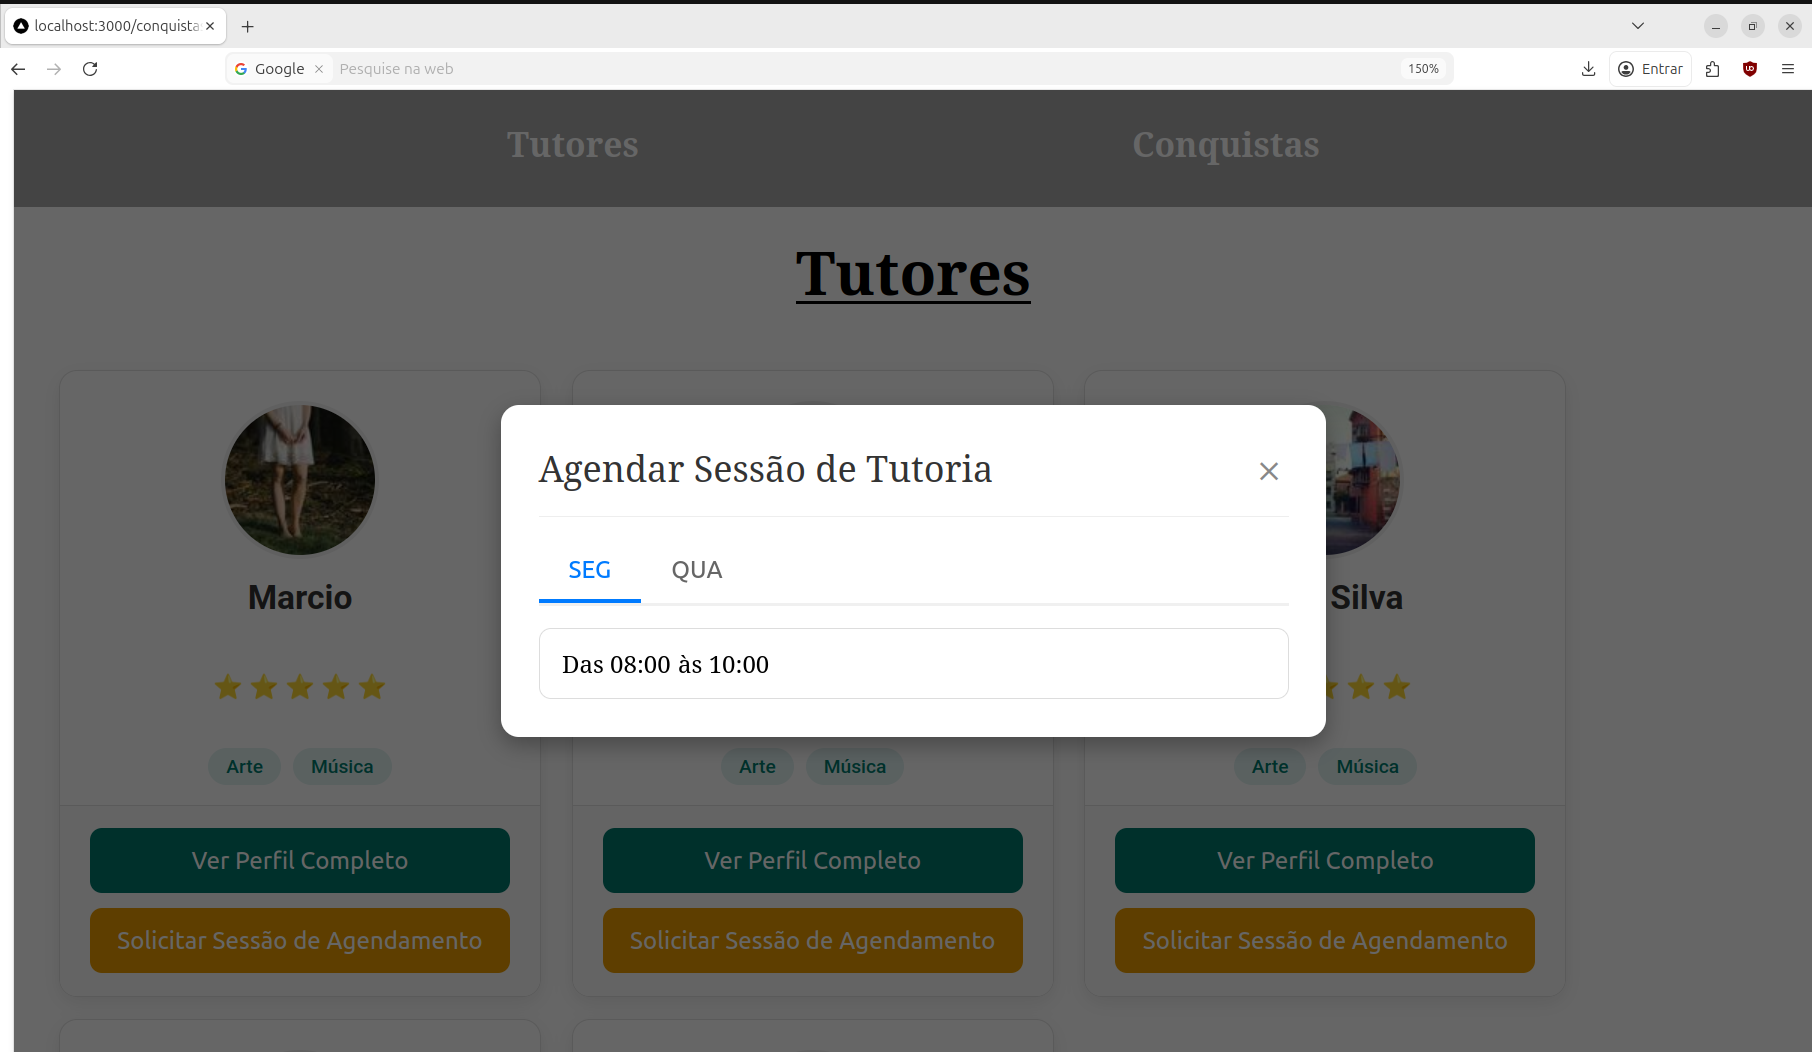
\includegraphics[width=0.99\textwidth]{figuras/sessao.png}


    Fonte: Autoria própria.
    
    \vspace{0.2cm}
        
    \label{fig:sessoes}
\end{figure}

Ao clicar em um horário, a solicitação de tutoria é realizada, a qual o tutor deve aceitar para que seja de fato confirmada. O usuário é notificado da realização da solicitação, conforme a Figura \ref{fig:notificacao-sessao}. Para melhor visualização, a janela de notificação pode ser vista isoladamente na Figura \ref{fig:notificacao-solitacao}. 

Como esta ação desbloqueia uma conquista, é exibida outra notificação, apresentada pela Figura \ref{fig:notificacao-conquista}. Para melhor visualização, a janela de notificação pode ser vista isoladamente na Figura \ref{fig:notificacao-conquista-isolada}. 

\newpage

\begin{figure}[h!]
    \centering

    \caption{Notificação de solicitação de tutoria.} 
    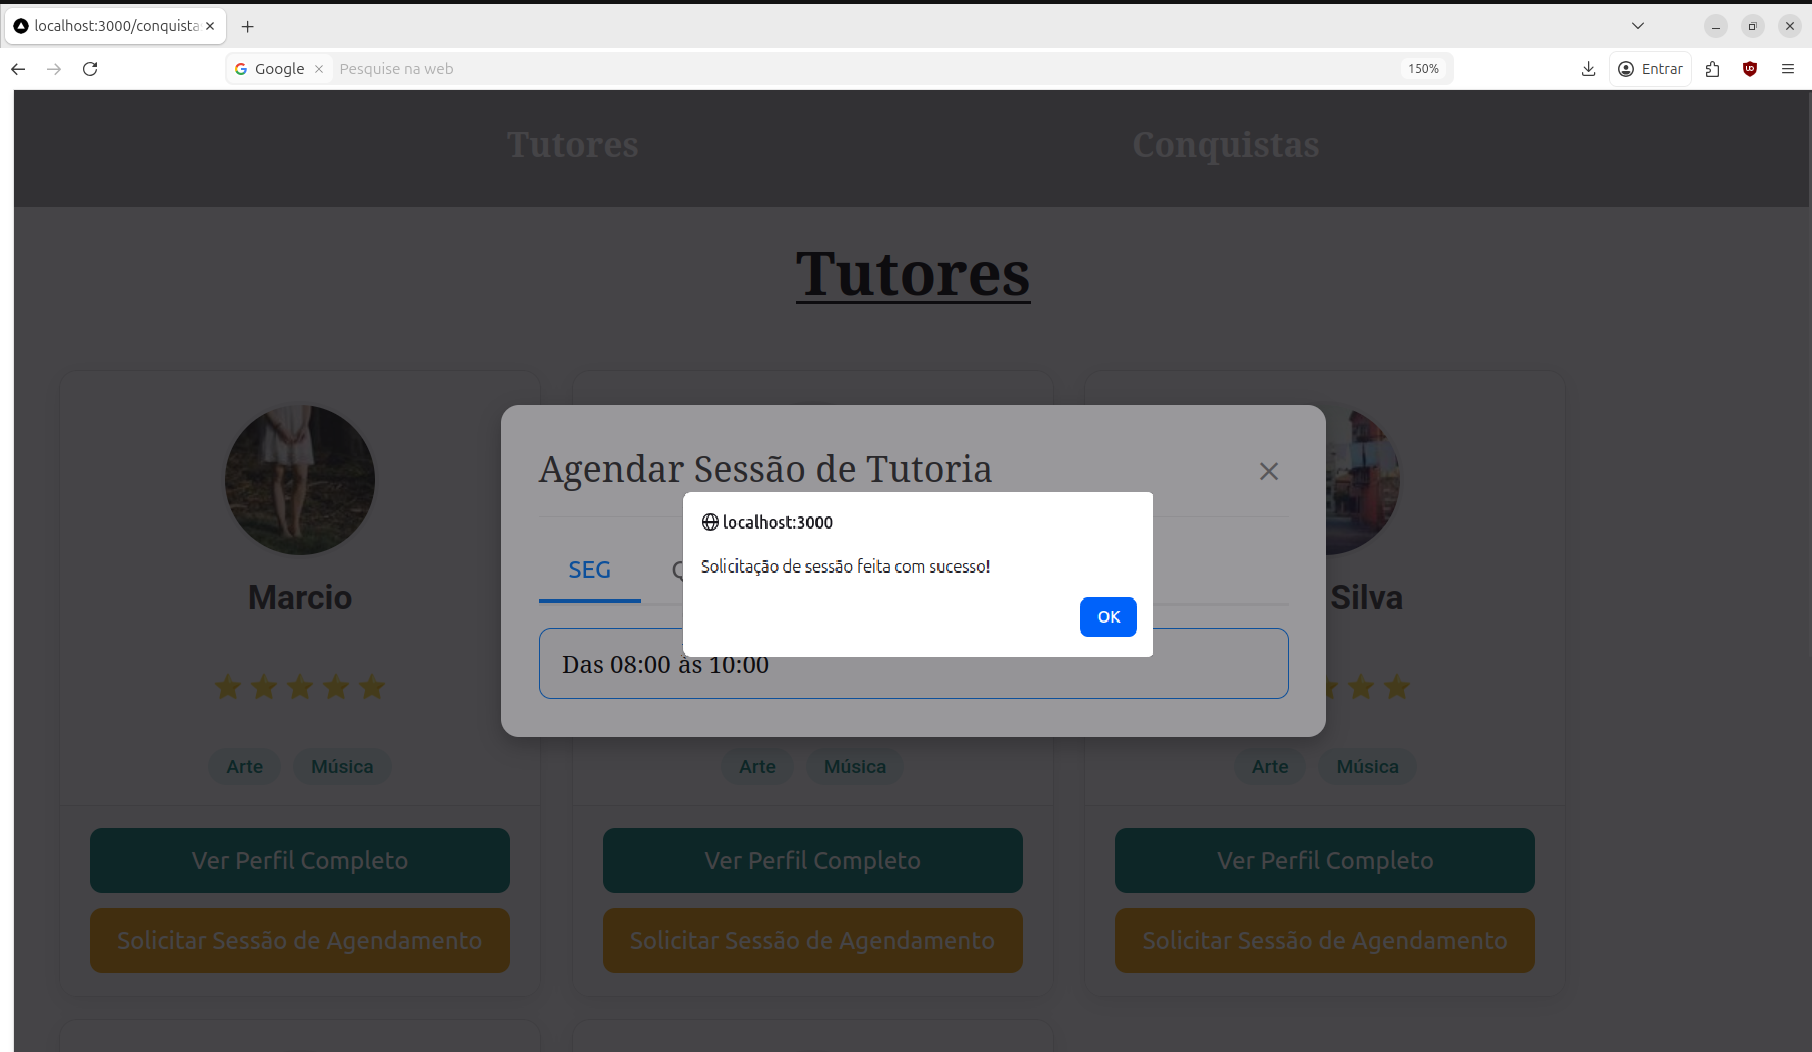
\includegraphics[width=0.99\textwidth]{figuras/notificacao-sessao.png}

    Fonte: Autoria própria.
    
    \vspace{0.2cm}
        
    \label{fig:notificacao-sessao}
\end{figure}

\begin{figure}[h!]
    \centering

    \caption{Janela de notificação de solicitação de tutoria.} 
    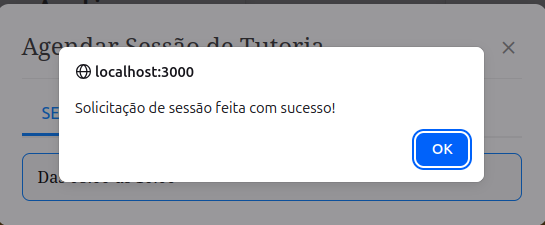
\includegraphics[width=0.75\textwidth]{figuras/notificacao-solitacao.png}

    Fonte: Autoria própria.
    
    \vspace{0.2cm}
        
    \label{fig:notificacao-solitacao}
\end{figure}

\newpage

\begin{figure}[h!]
    \centering

    \caption{Notificação de desbloqueio da conquista.} 
    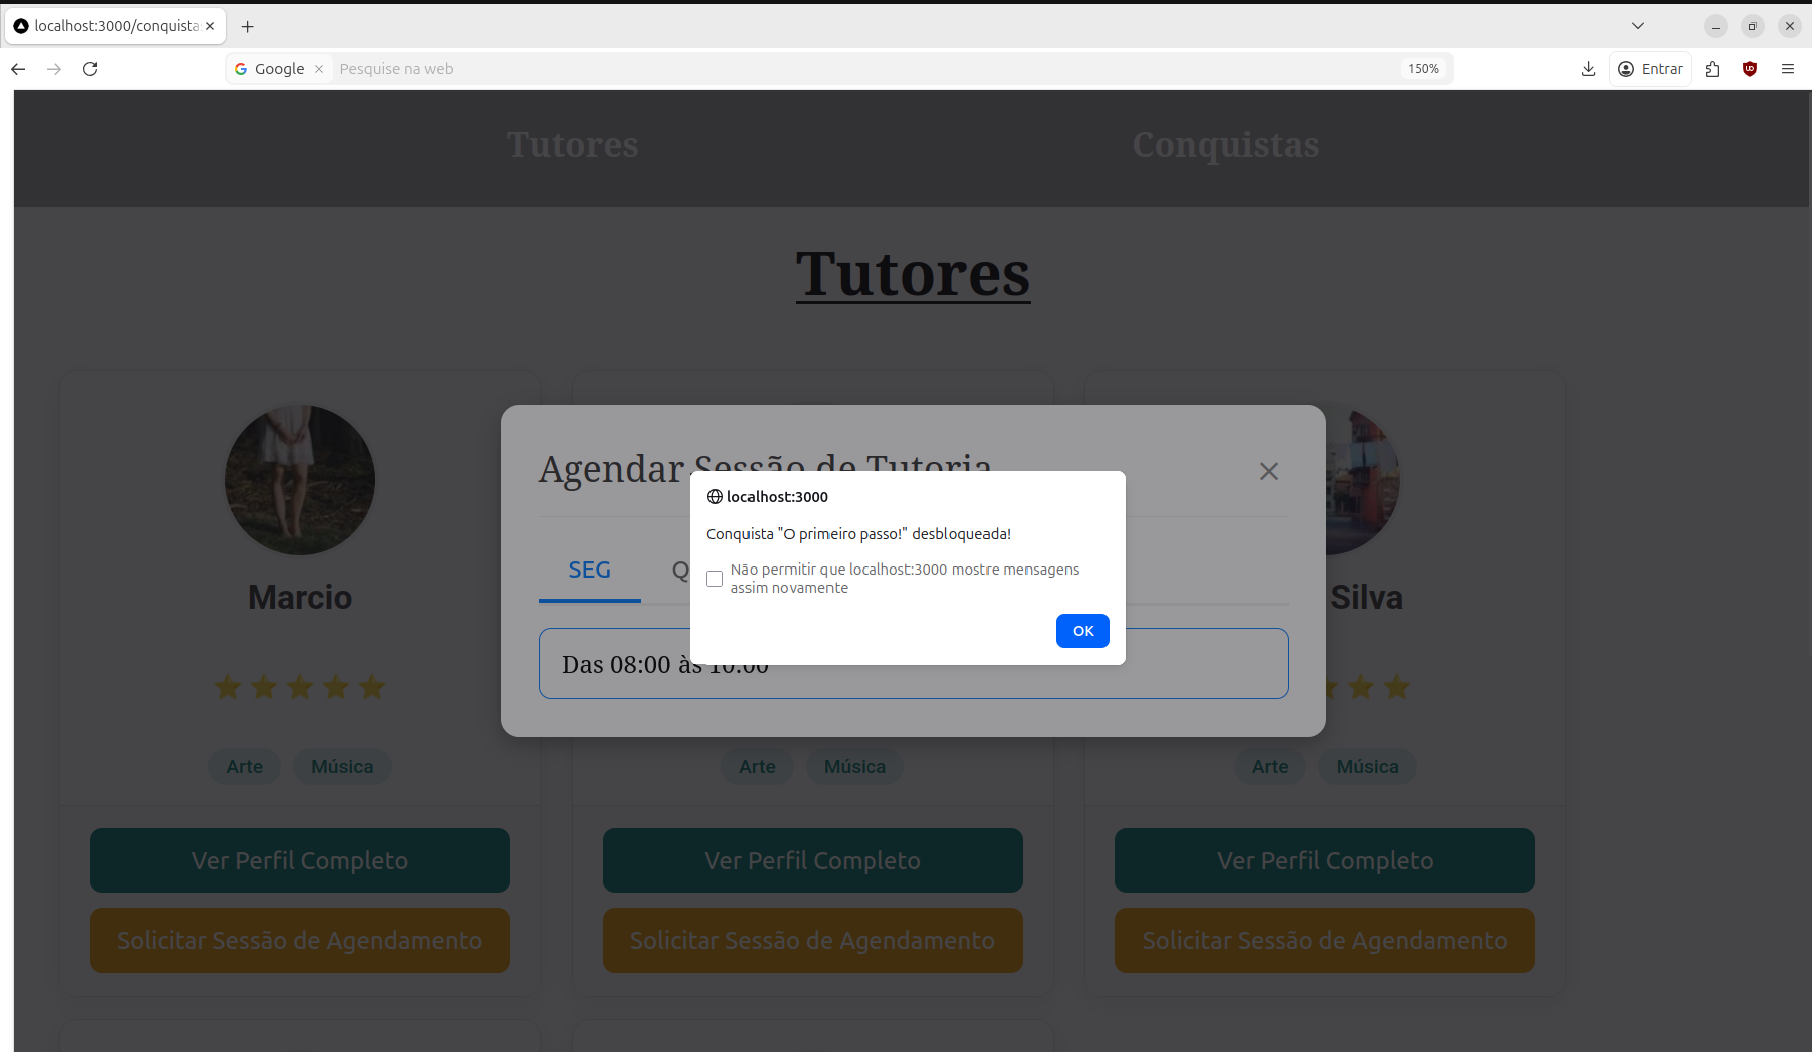
\includegraphics[width=0.99\textwidth]{figuras/notificacao-conquista.png}

    Fonte: Autoria própria.
    
    \vspace{0.2cm}
        
    \label{fig:notificacao-conquista}
\end{figure}

\begin{figure}[h!]
    \centering

    \caption{Janela de notificação de desbloqueio de conquistas.} 
    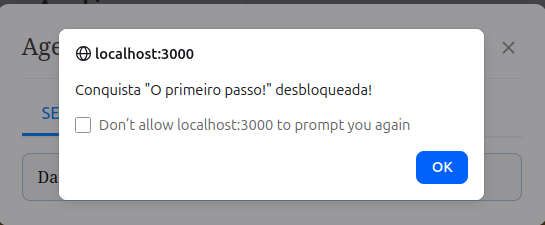
\includegraphics[width=0.75\textwidth]{figuras/notificacao-conquista-isolada.png}

    Fonte: Autoria própria.
    
    \vspace{0.2cm}
        
    \label{fig:notificacao-conquista-isolada}
\end{figure}

Ao voltar para a tela de conquistas, a conquista desbloqueada é apresentada em cores, conforme mostra a Figura \ref{fig:conquista-liberada}.

\newpage

\begin{figure}[h!]
    \centering
    \caption{Conquista desbloqueada.} 
    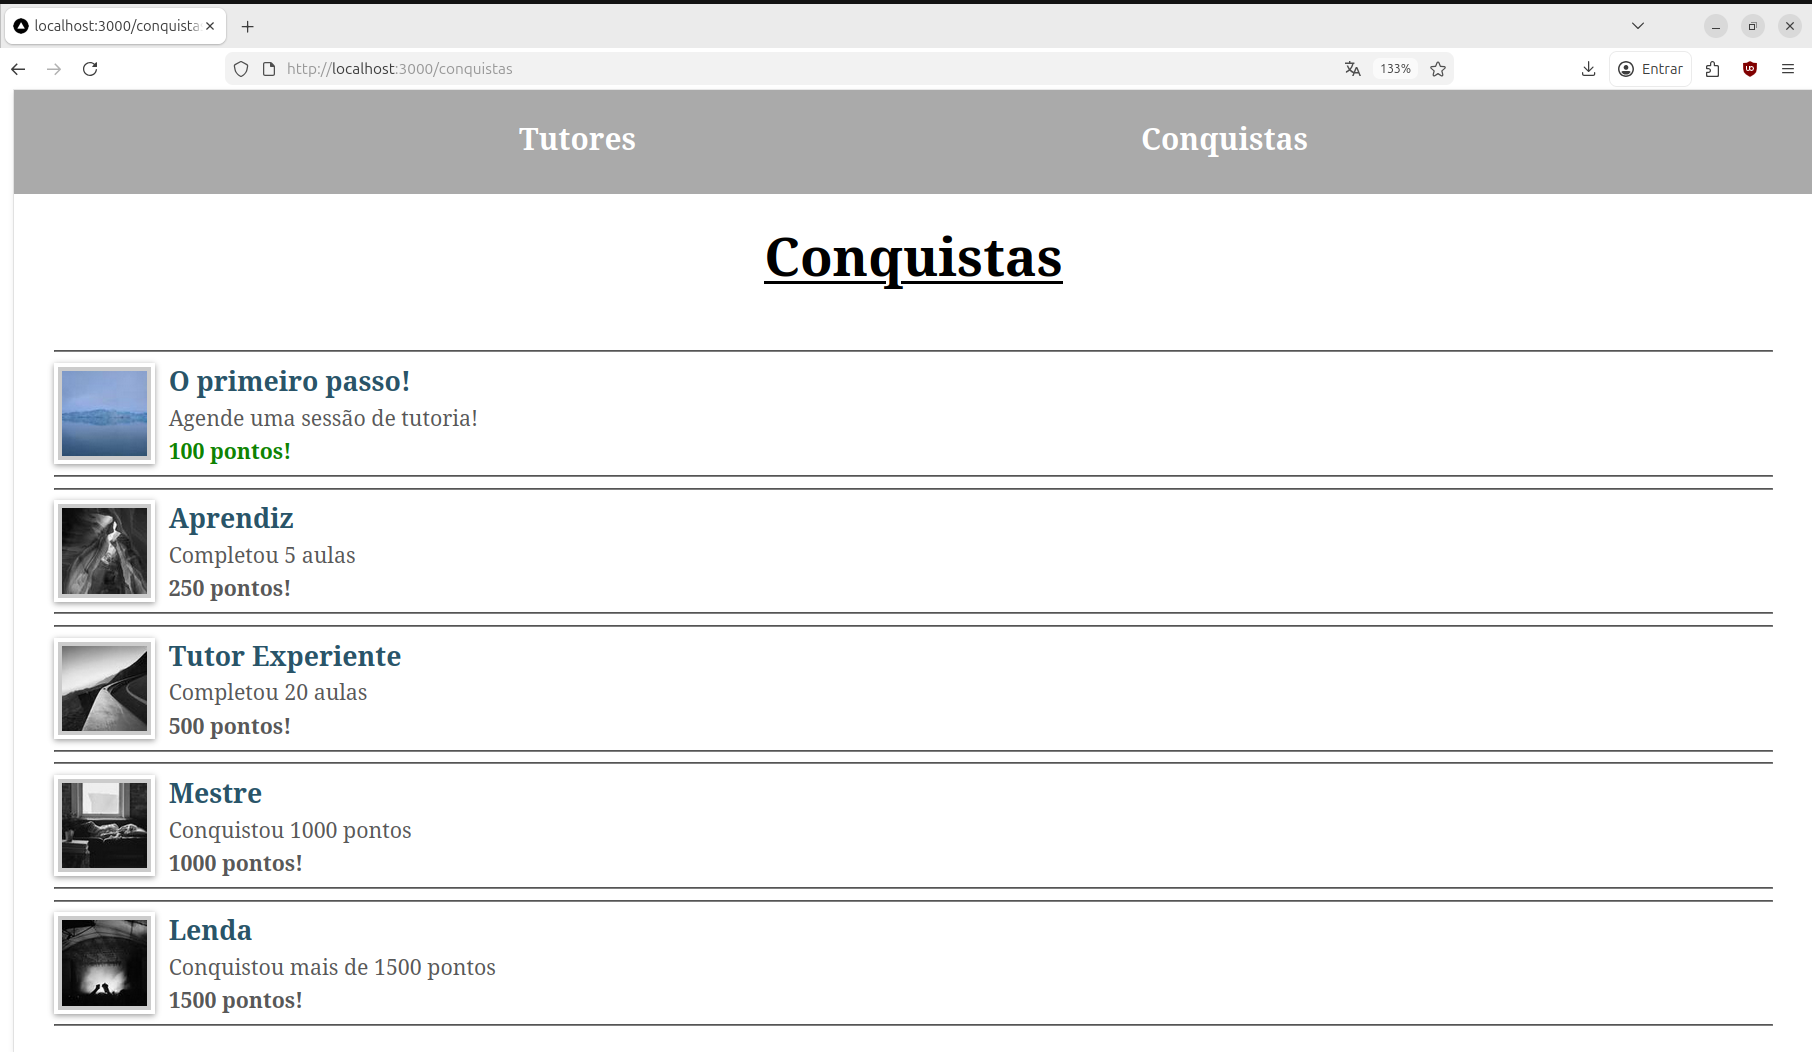
\includegraphics[width=0.99\textwidth]{figuras/conquista-liberada.png}


    Fonte: Autoria própria.
    
    \vspace{0.2cm}
        
    \label{fig:conquista-liberada}
\end{figure}

A simulação tornou possível perceber que a arquitetura proposta consegue realizar a integração entre o \textit{backend} e o \textit{frontend} de forma satisfatória, além de demonstrar a capacidade de realizar consultas e registros na base de dados modelada. Assim, a arquitetura atende as
necessidades da proposta e é viável para o desenvolvimento do projeto.


\chapter[\textit{Lean Inception}]{\textit{Lean Inception}}
\label{lean-inception}

O \textit{Lean Inception} foi desenvolvido no Figma, adaptado a partir do template disponível em \href{caroli.org}{caroli.org}, podendo ser acessado pelo \href{https://www.figma.com/board/xXIvddv95LAyy0uTLGtEIc/TCC-Vandor?node-id=0-1&t=AienmrKhFTuCnwu8-1}{link}.

\begin{figure}[h!]
    \centering
    \caption{Visão do Produto.} 
    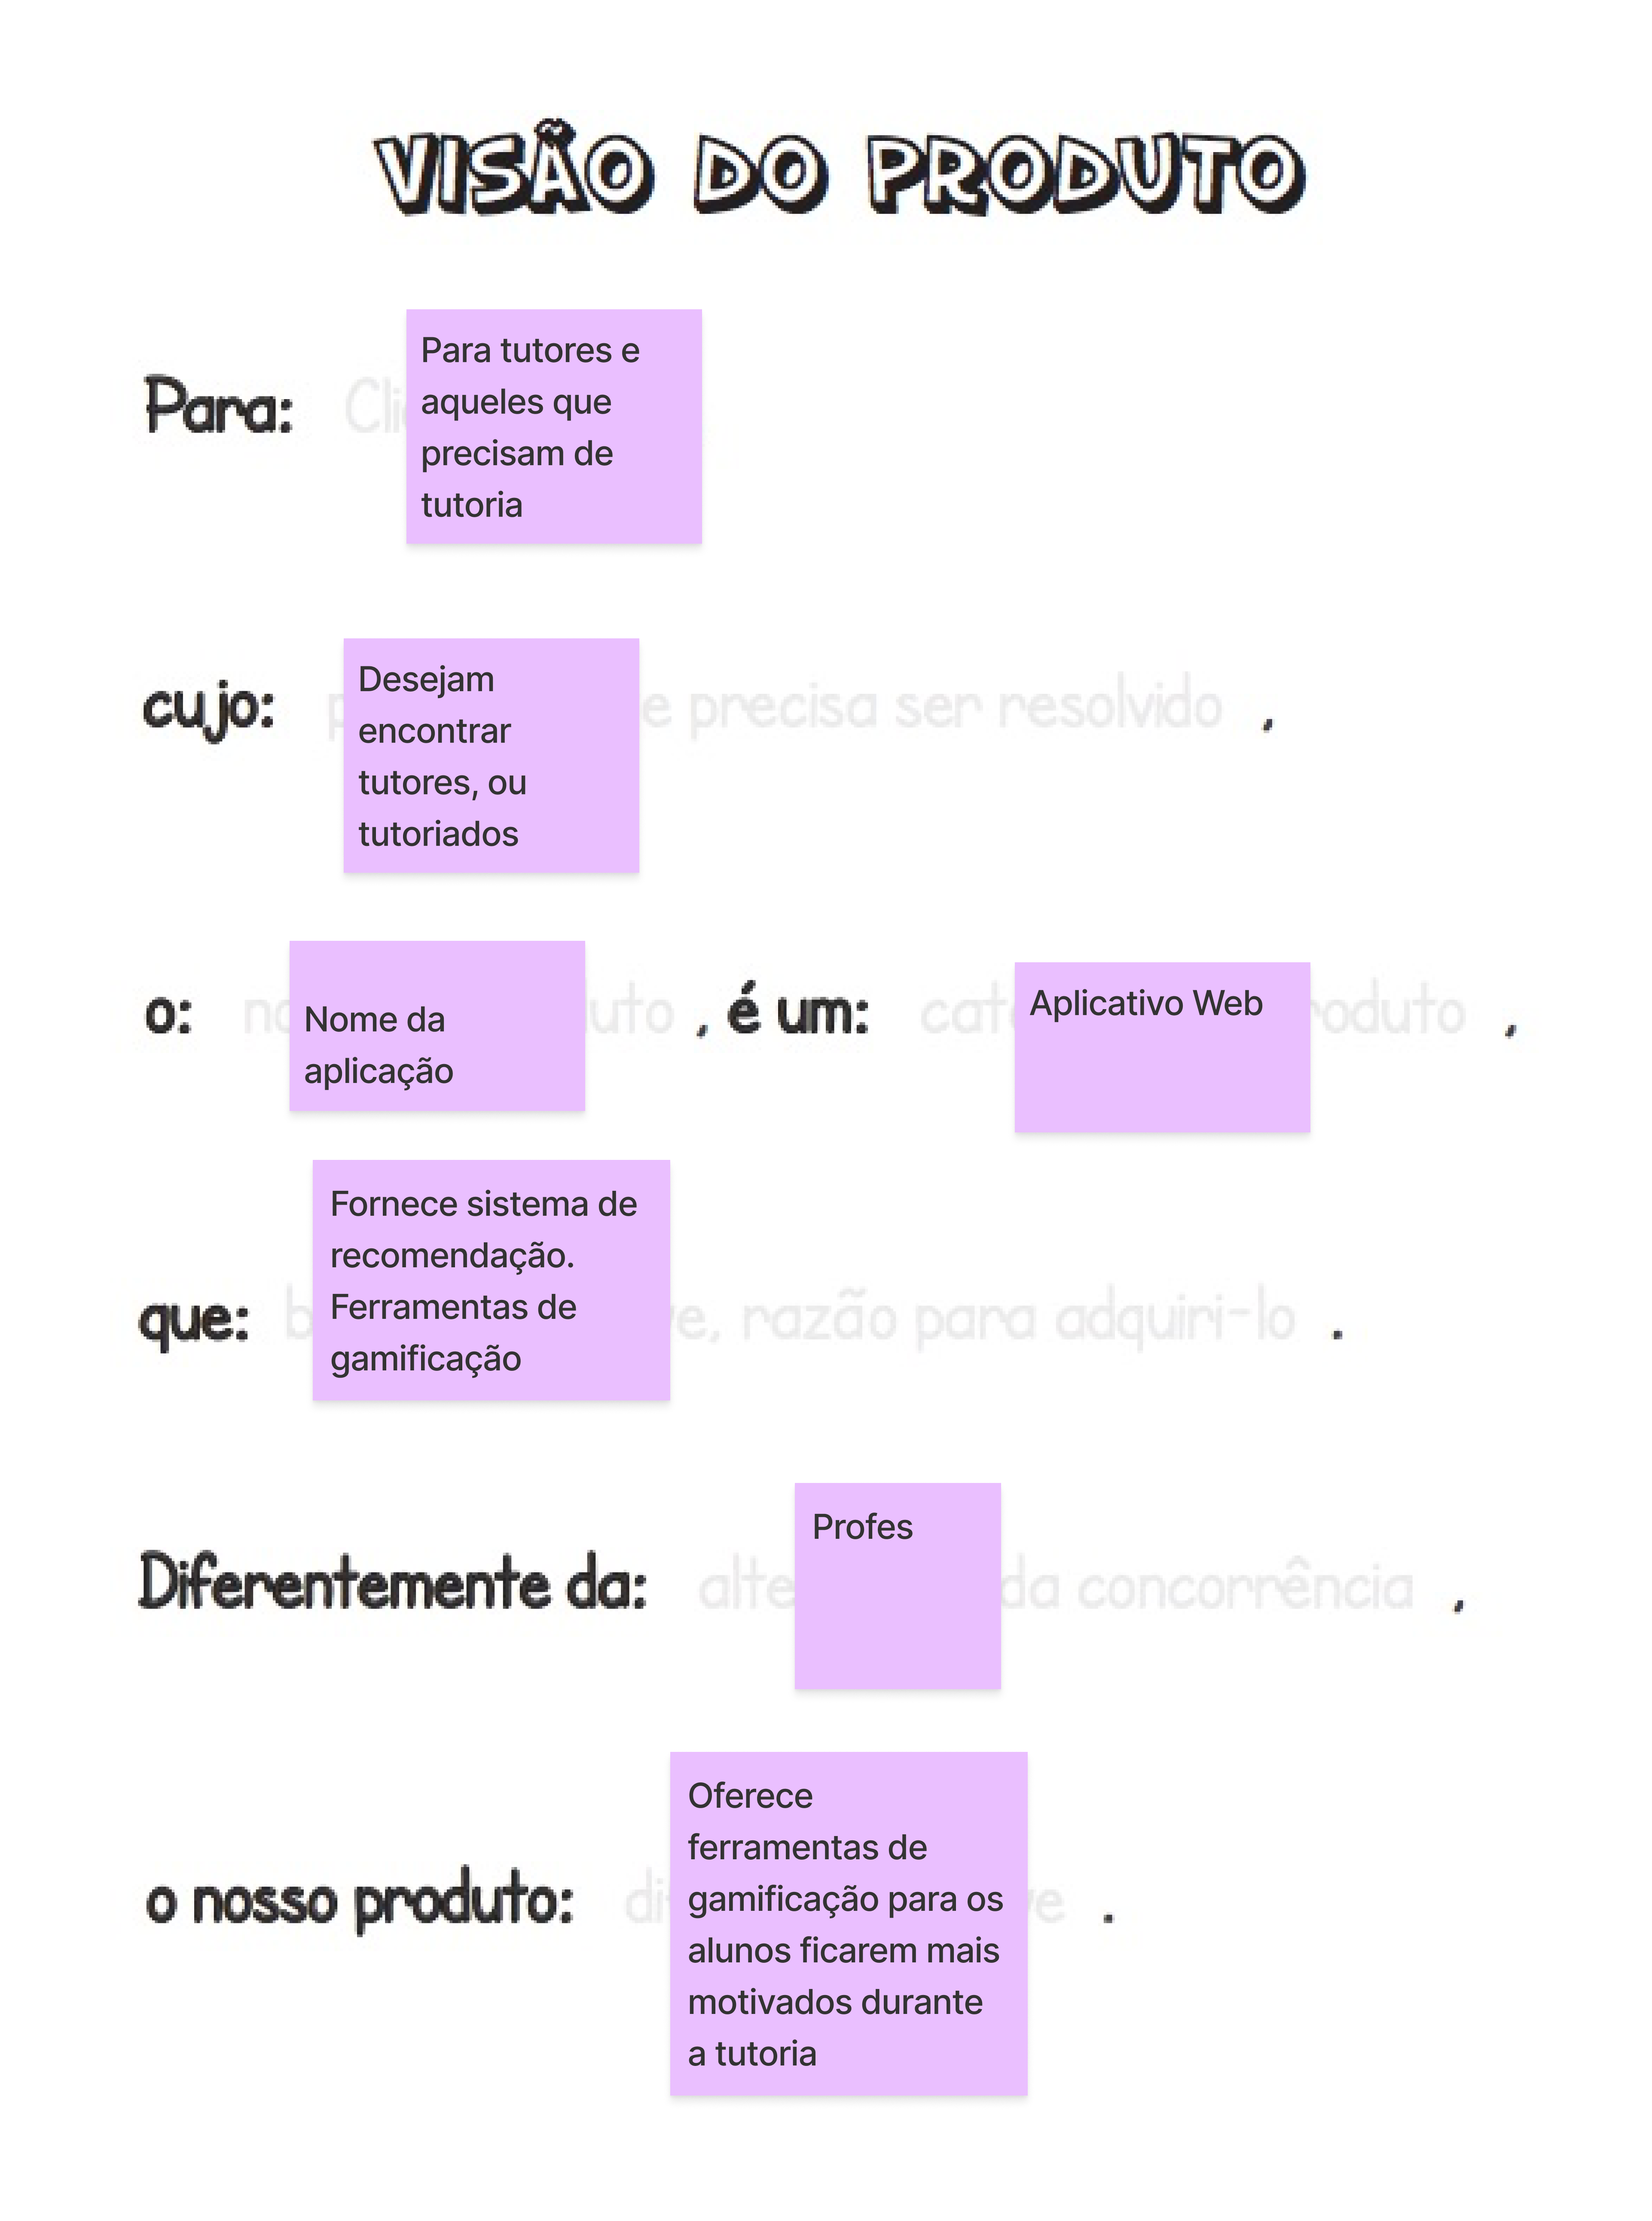
\includegraphics[width=0.9\textwidth]{figuras/Lean01VisaoProduto.png}

    Fonte: Adaptado a partir de caroli.org
    
    \vspace{0.2cm}
\end{figure}

\begin{figure}[h!]
    \centering
    \caption{Seção do que o software é.} 
    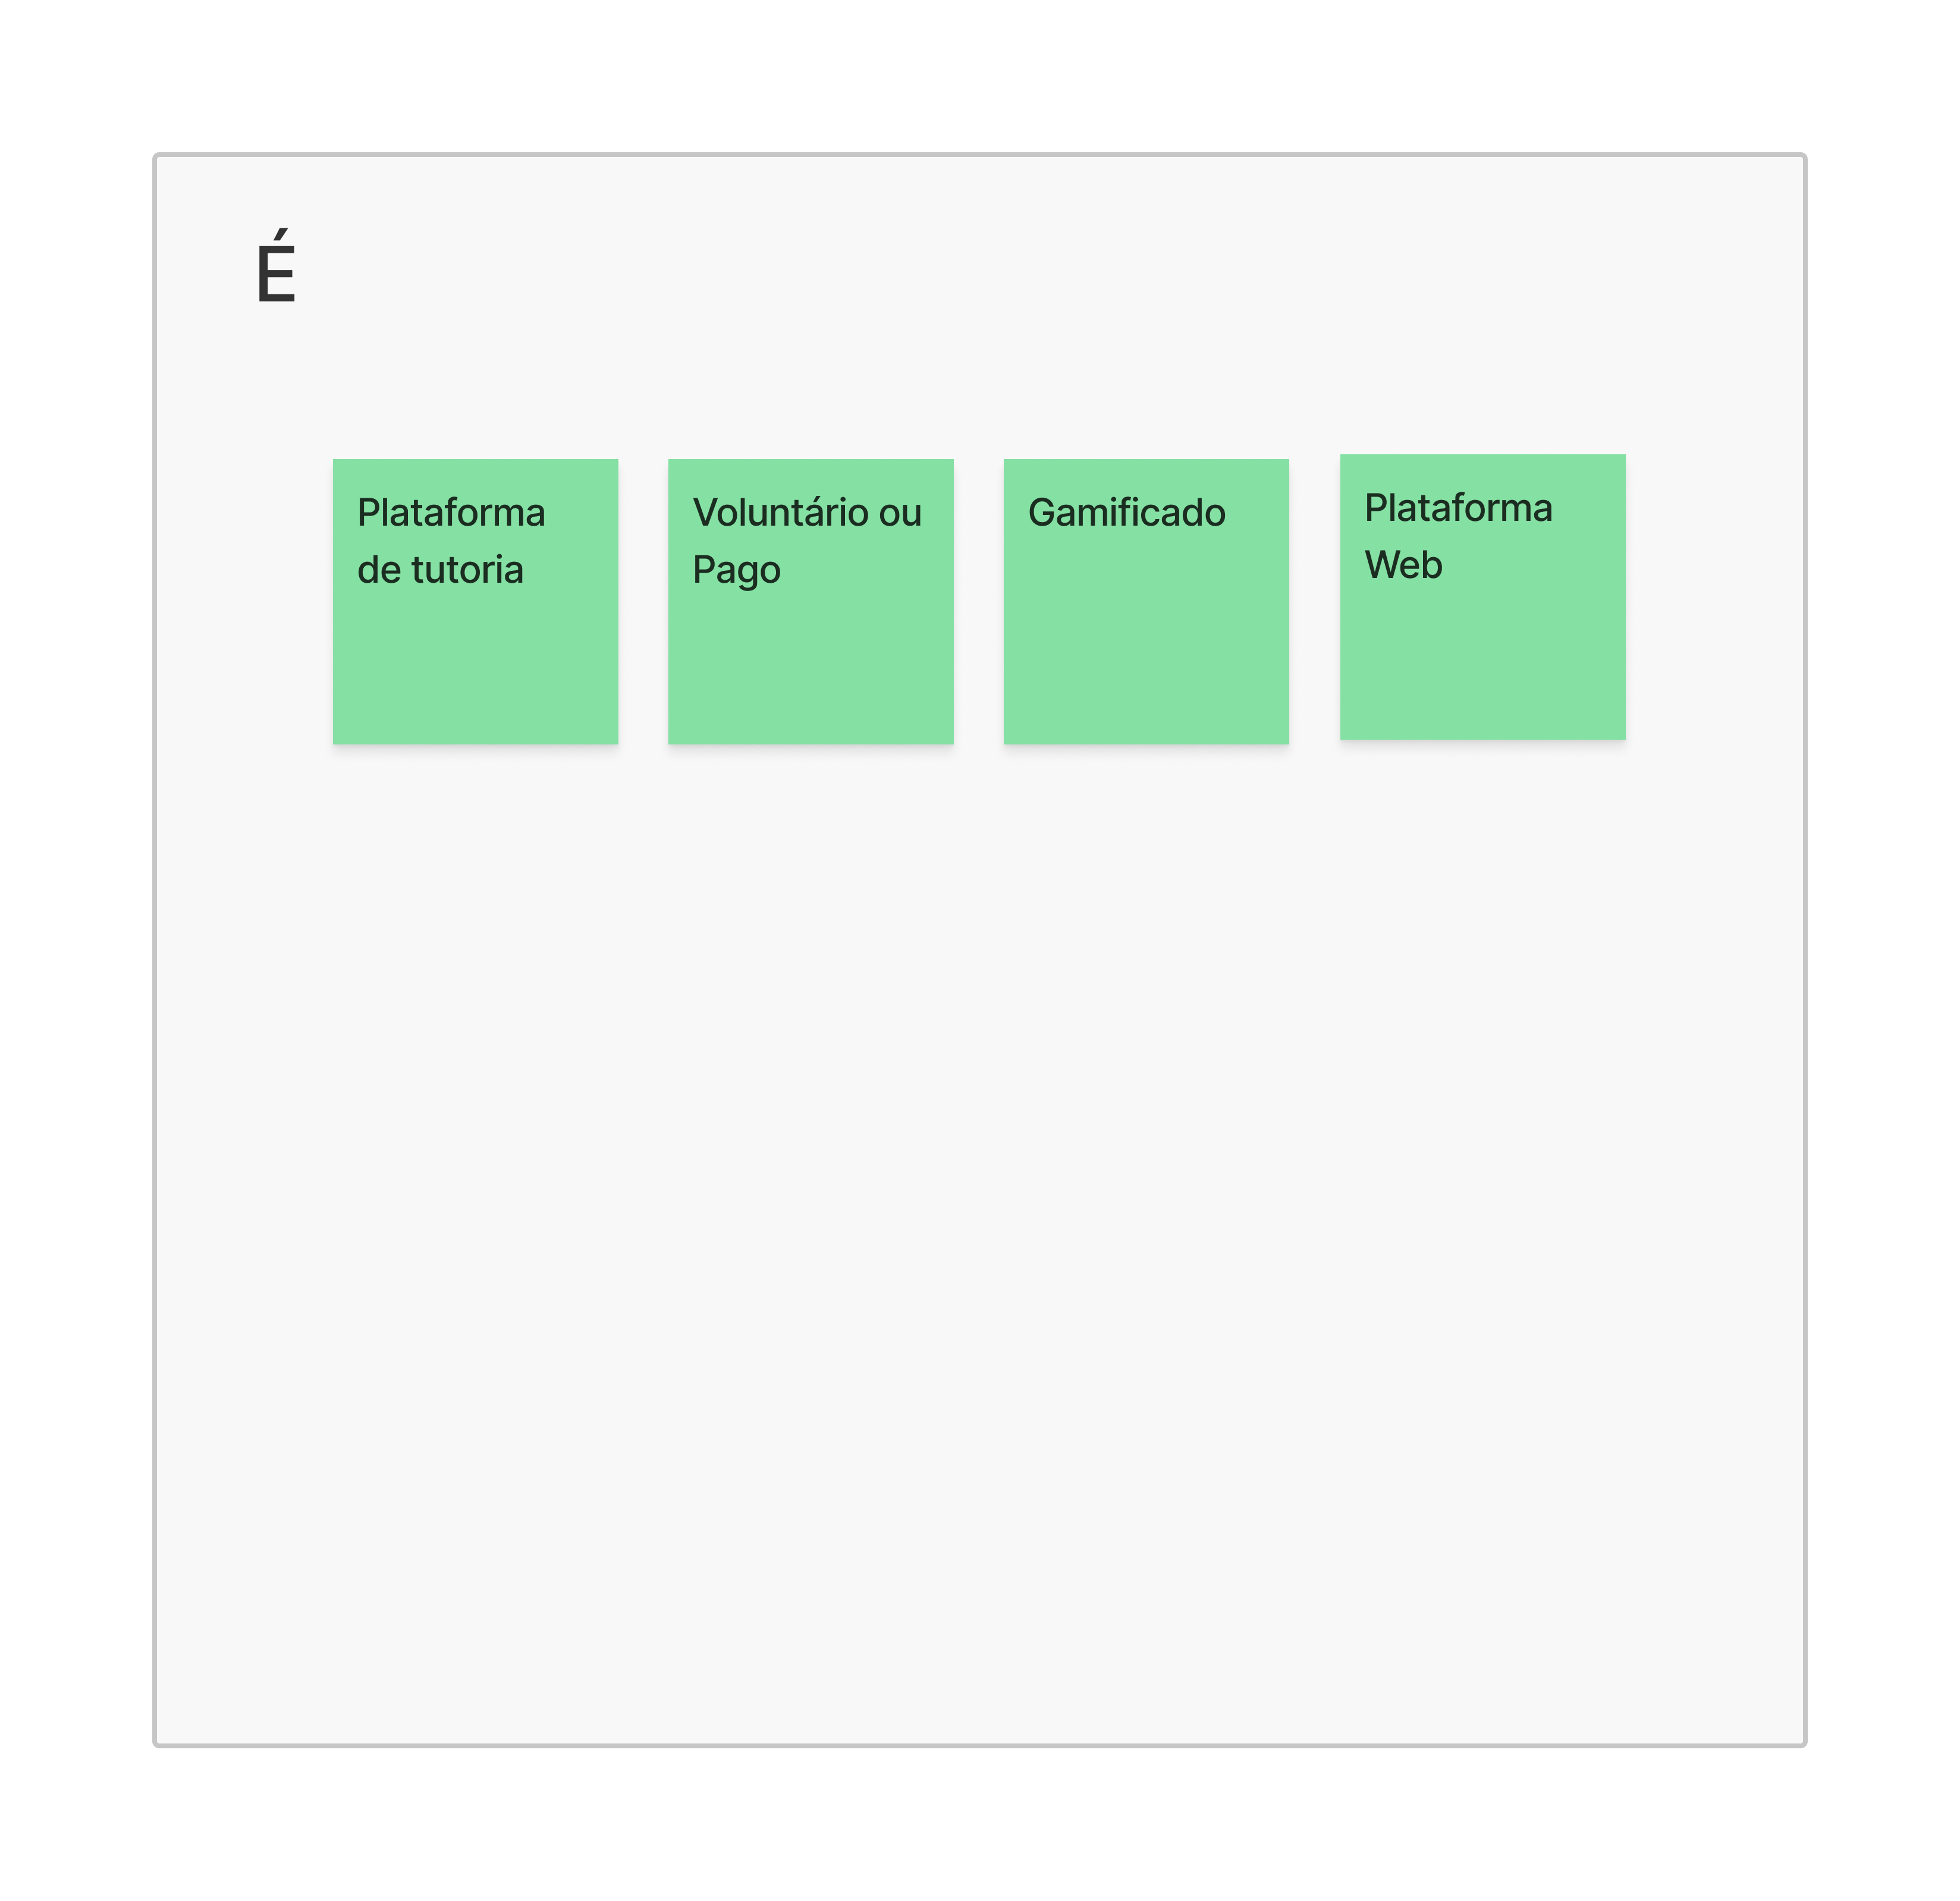
\includegraphics[width=0.9\textwidth]{figuras/Lean02Eh.png}
       
    Fonte: Adaptado a partir de caroli.org
    
    \vspace{0.2cm}
\end{figure}

\begin{figure}[h!]
    \centering
    \caption{Seção do que o software não é.} 
    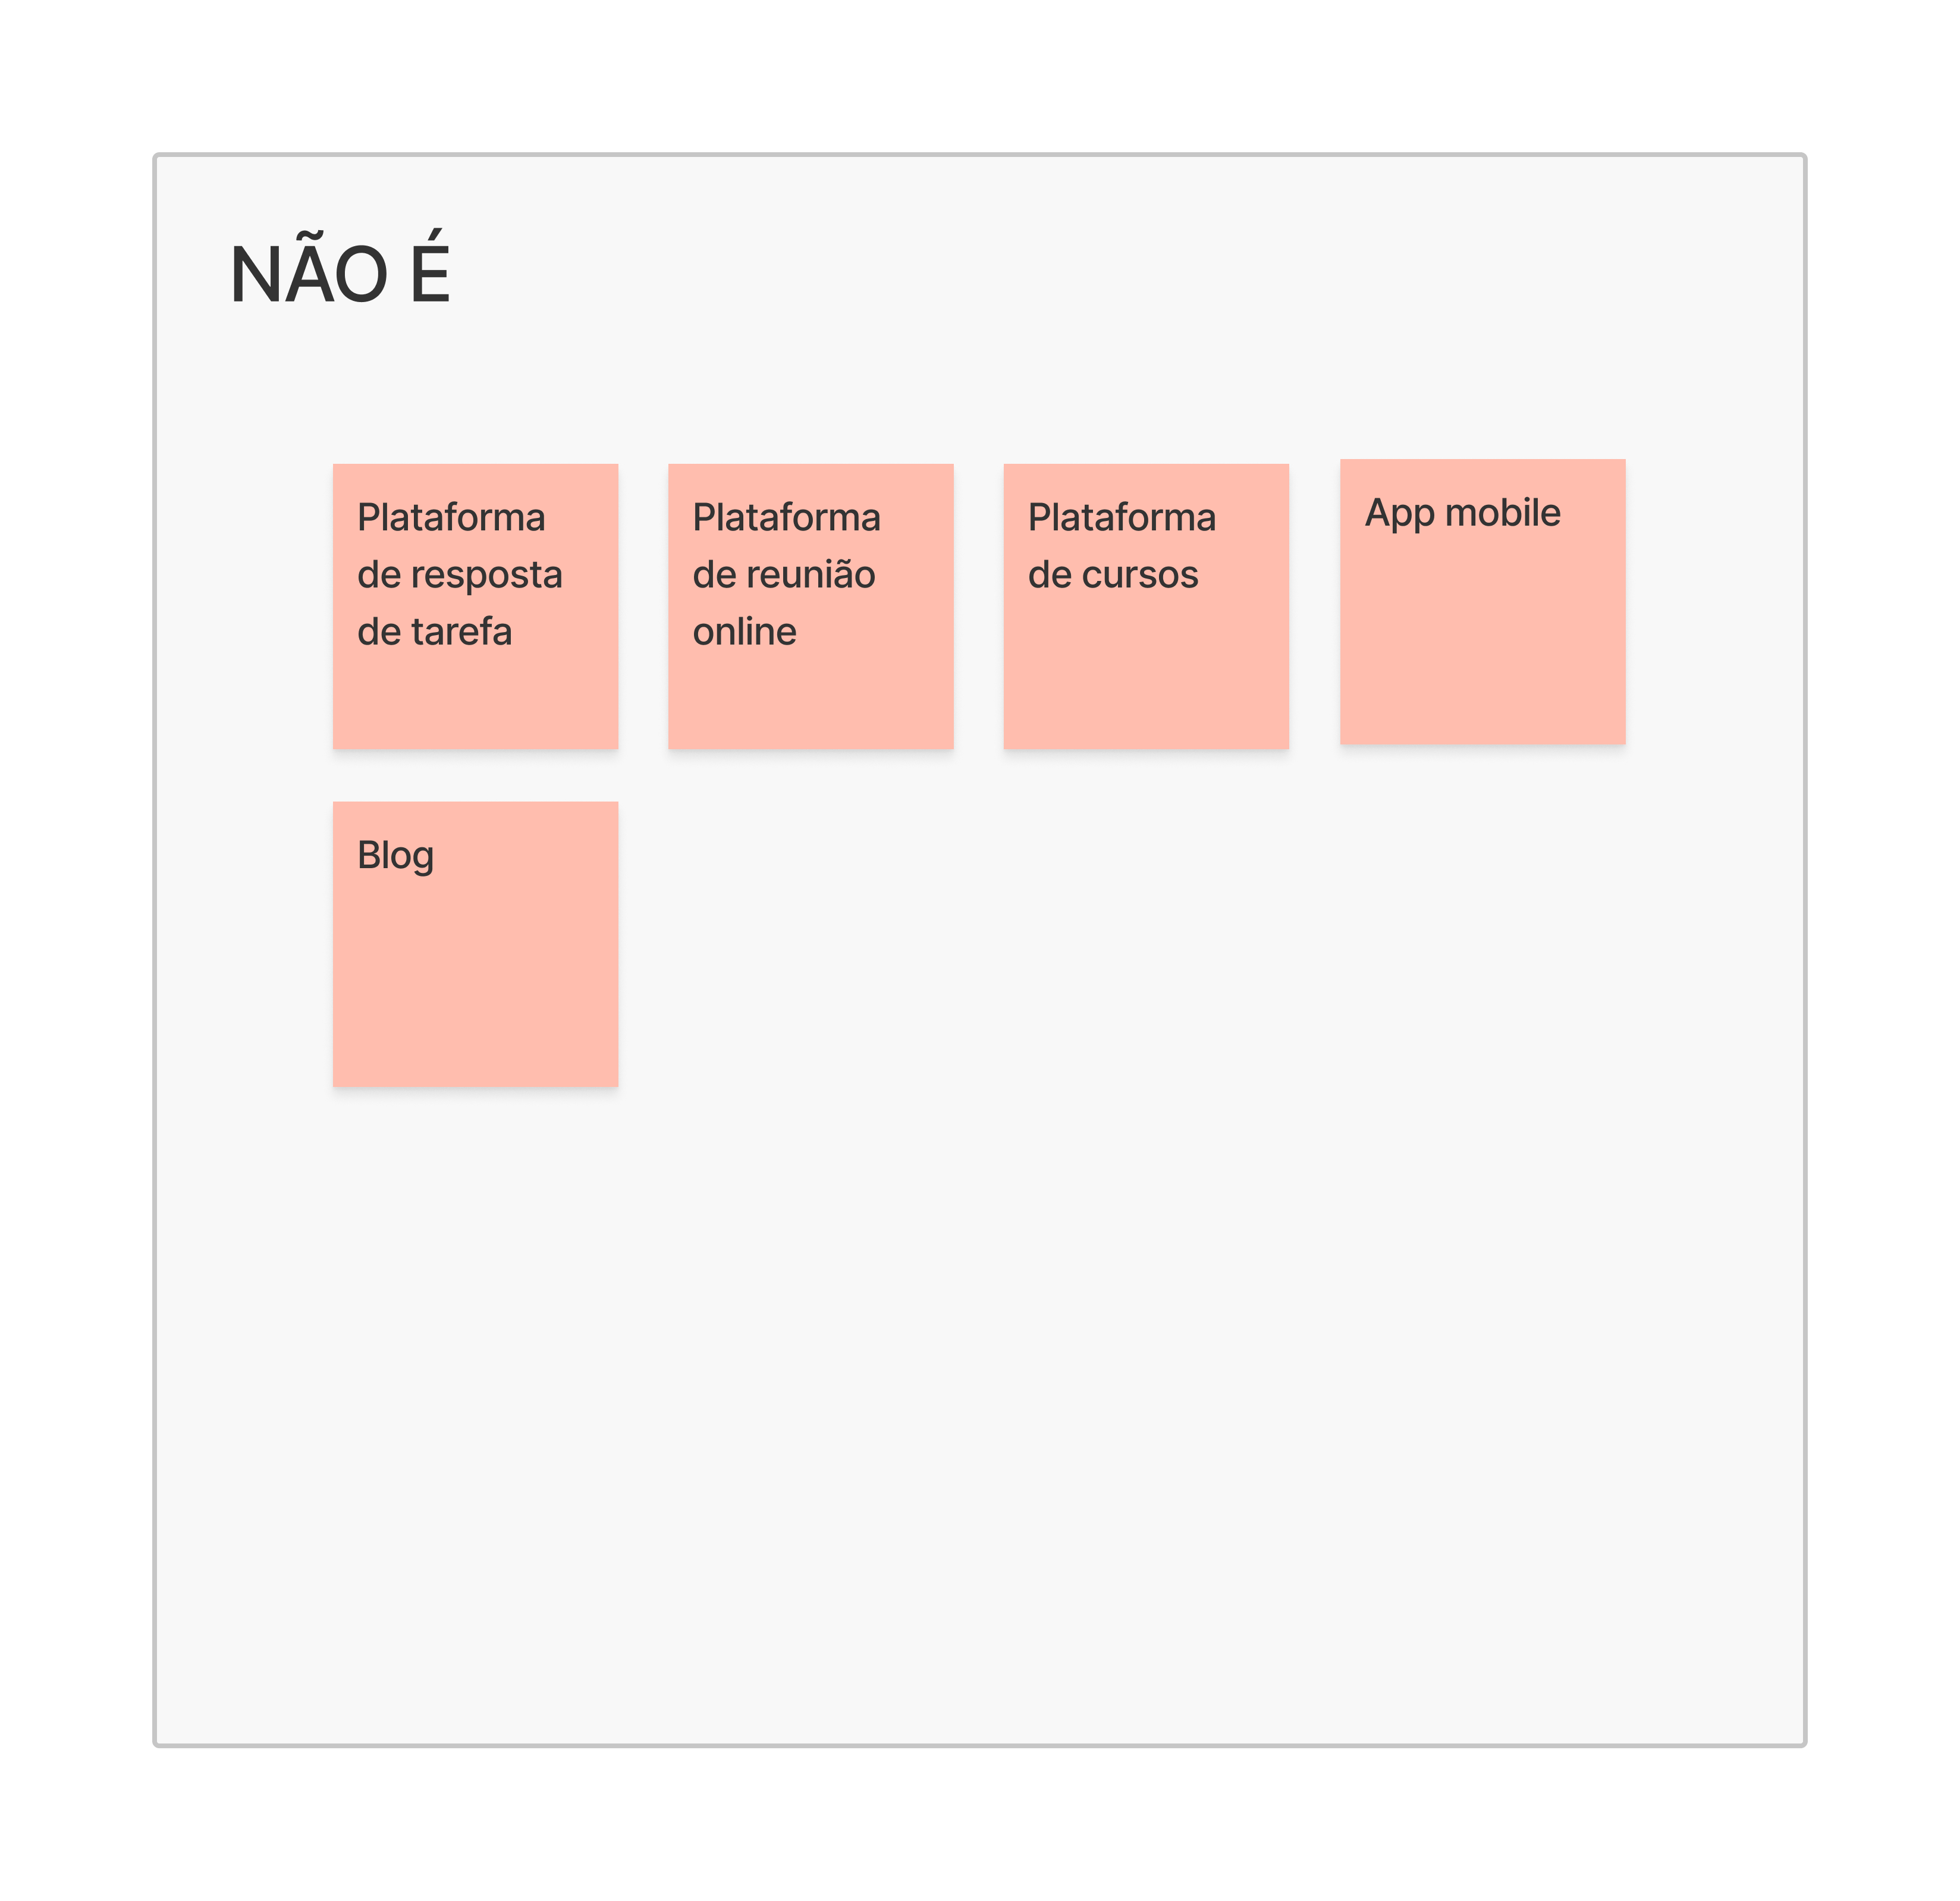
\includegraphics[width=0.9\textwidth]{figuras/Lean02NaoEh.png}

    Fonte: Adaptado a partir de caroli.org

    
    \vspace{0.2cm}
\end{figure}

\begin{figure}[h!]
    \centering
    \caption{Seção do que o software faz.} 
    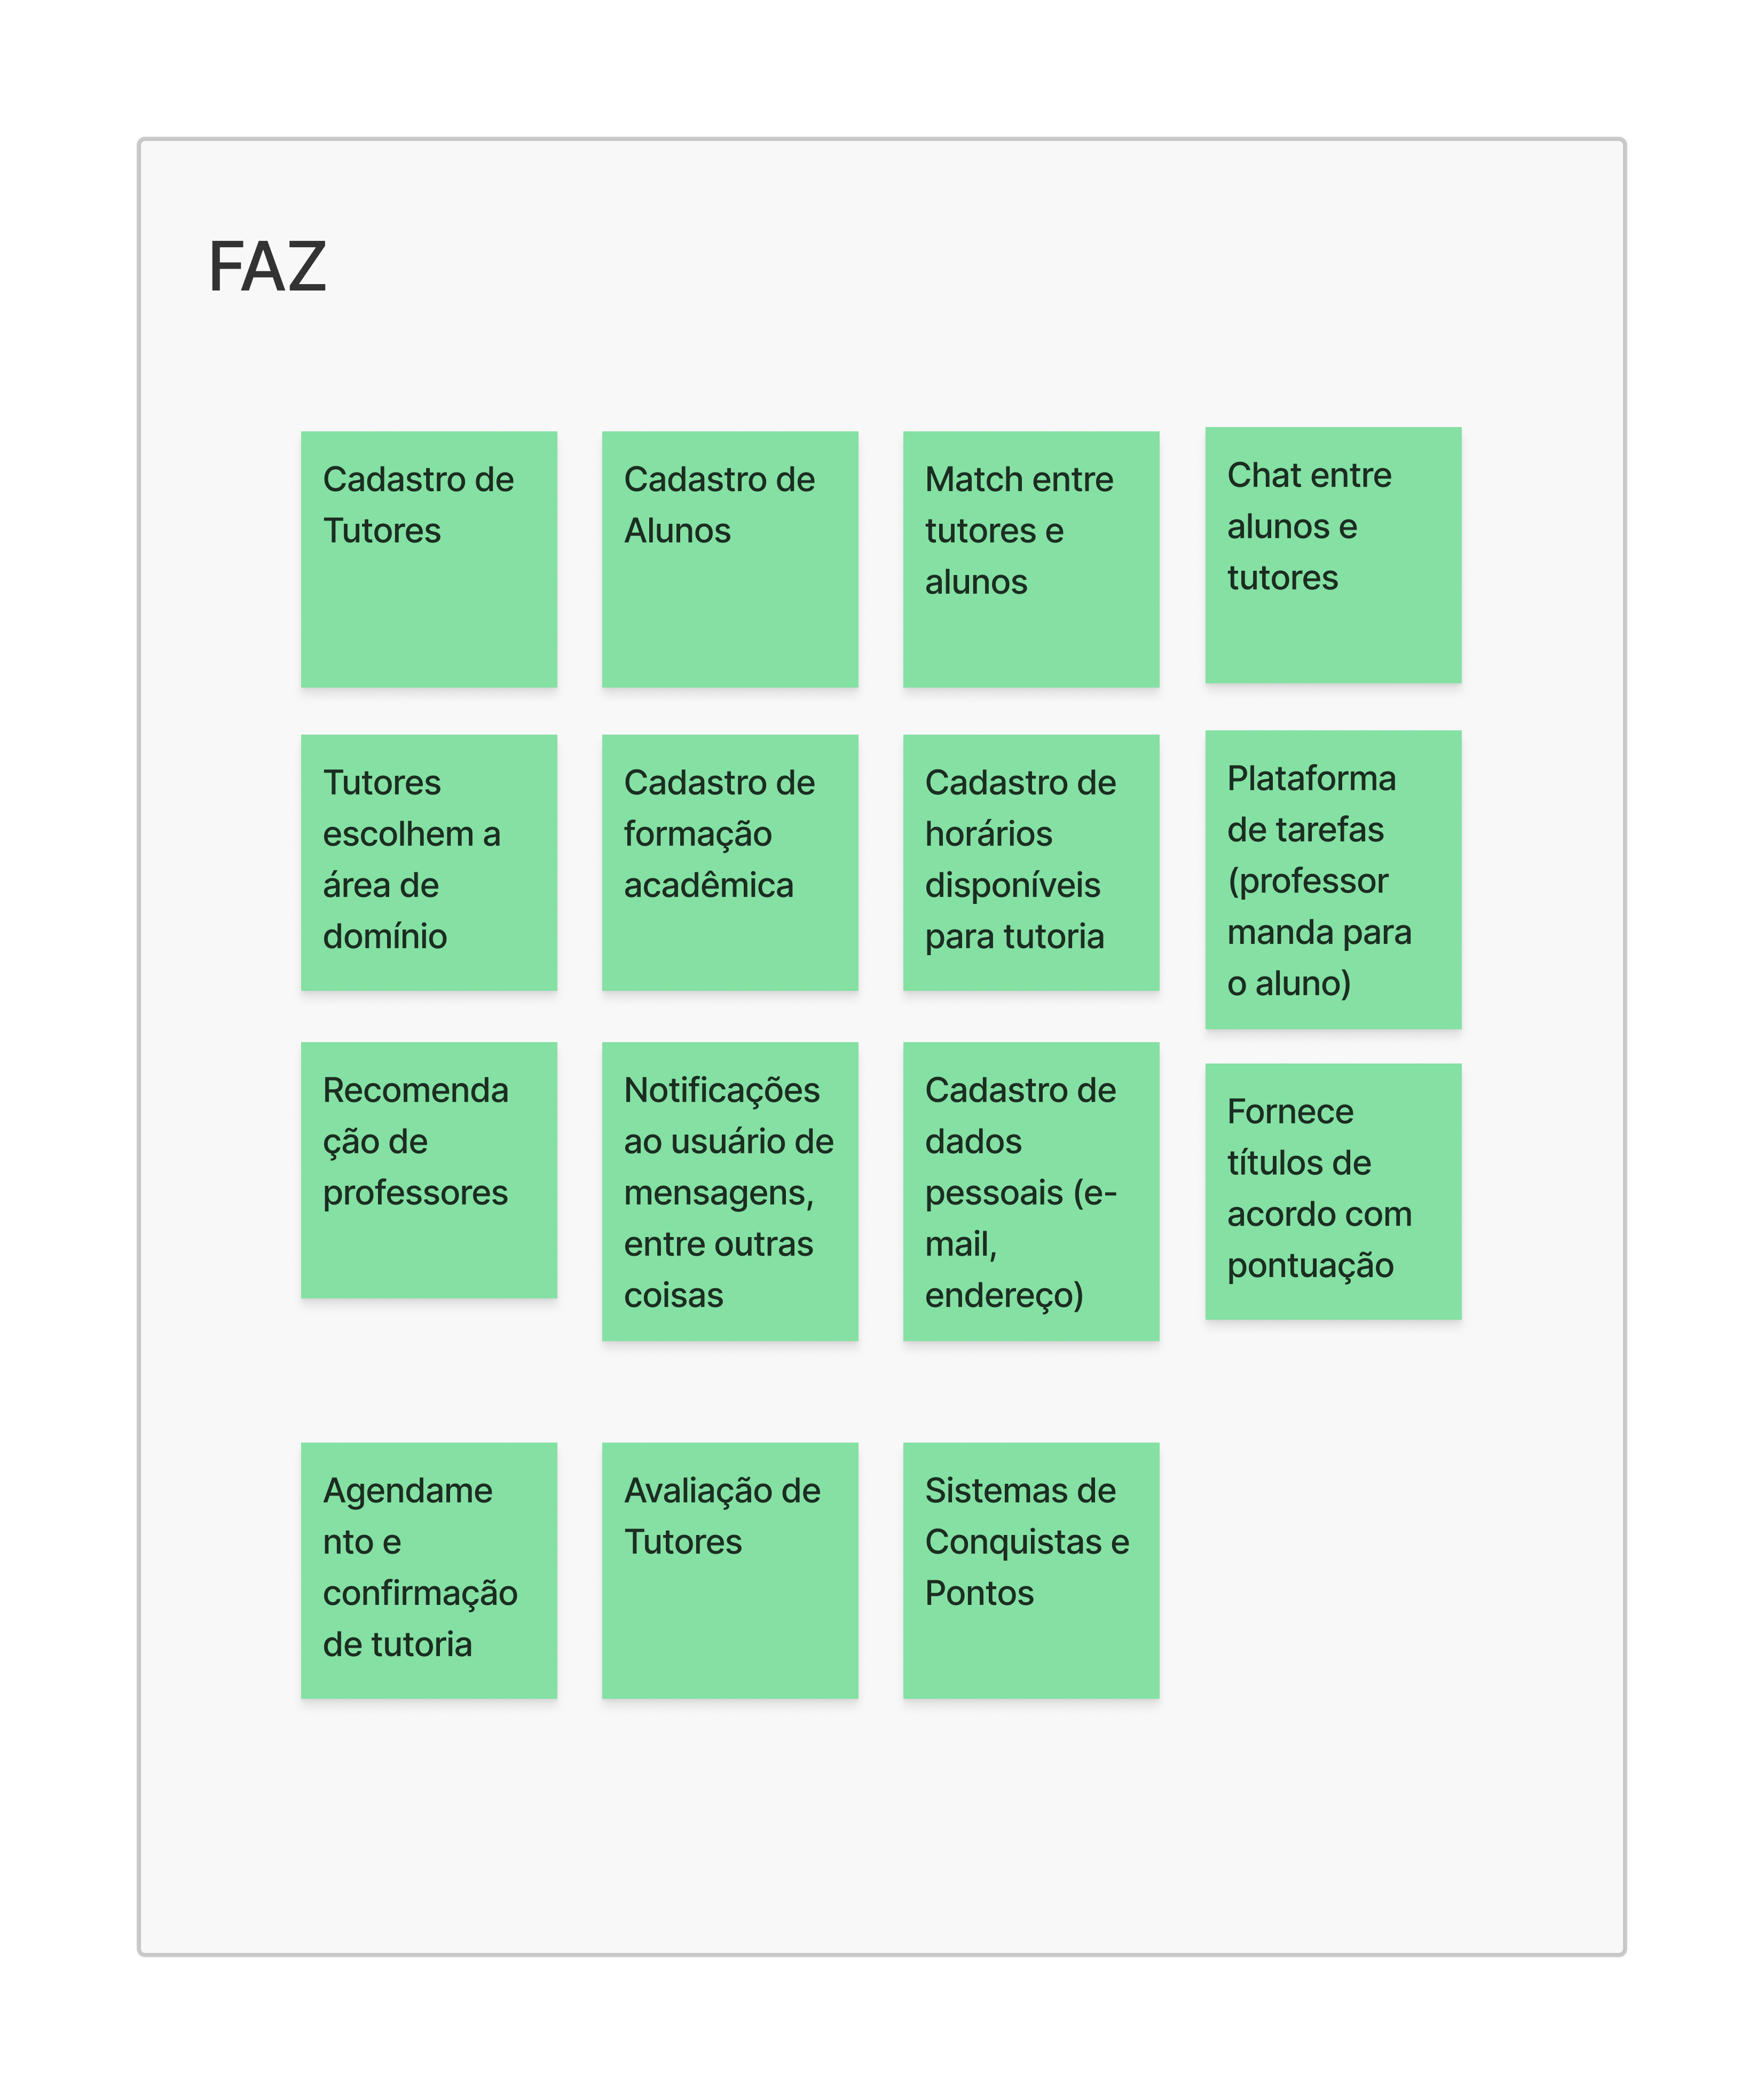
\includegraphics[width=0.9\textwidth]{figuras/Lean02Faz.png}

    Fonte: Adaptado a partir de caroli.org
    
    \vspace{0.2cm}
\end{figure}

\begin{figure}[h!]
    \centering
    \caption{Seção do que o software não faz.} 
    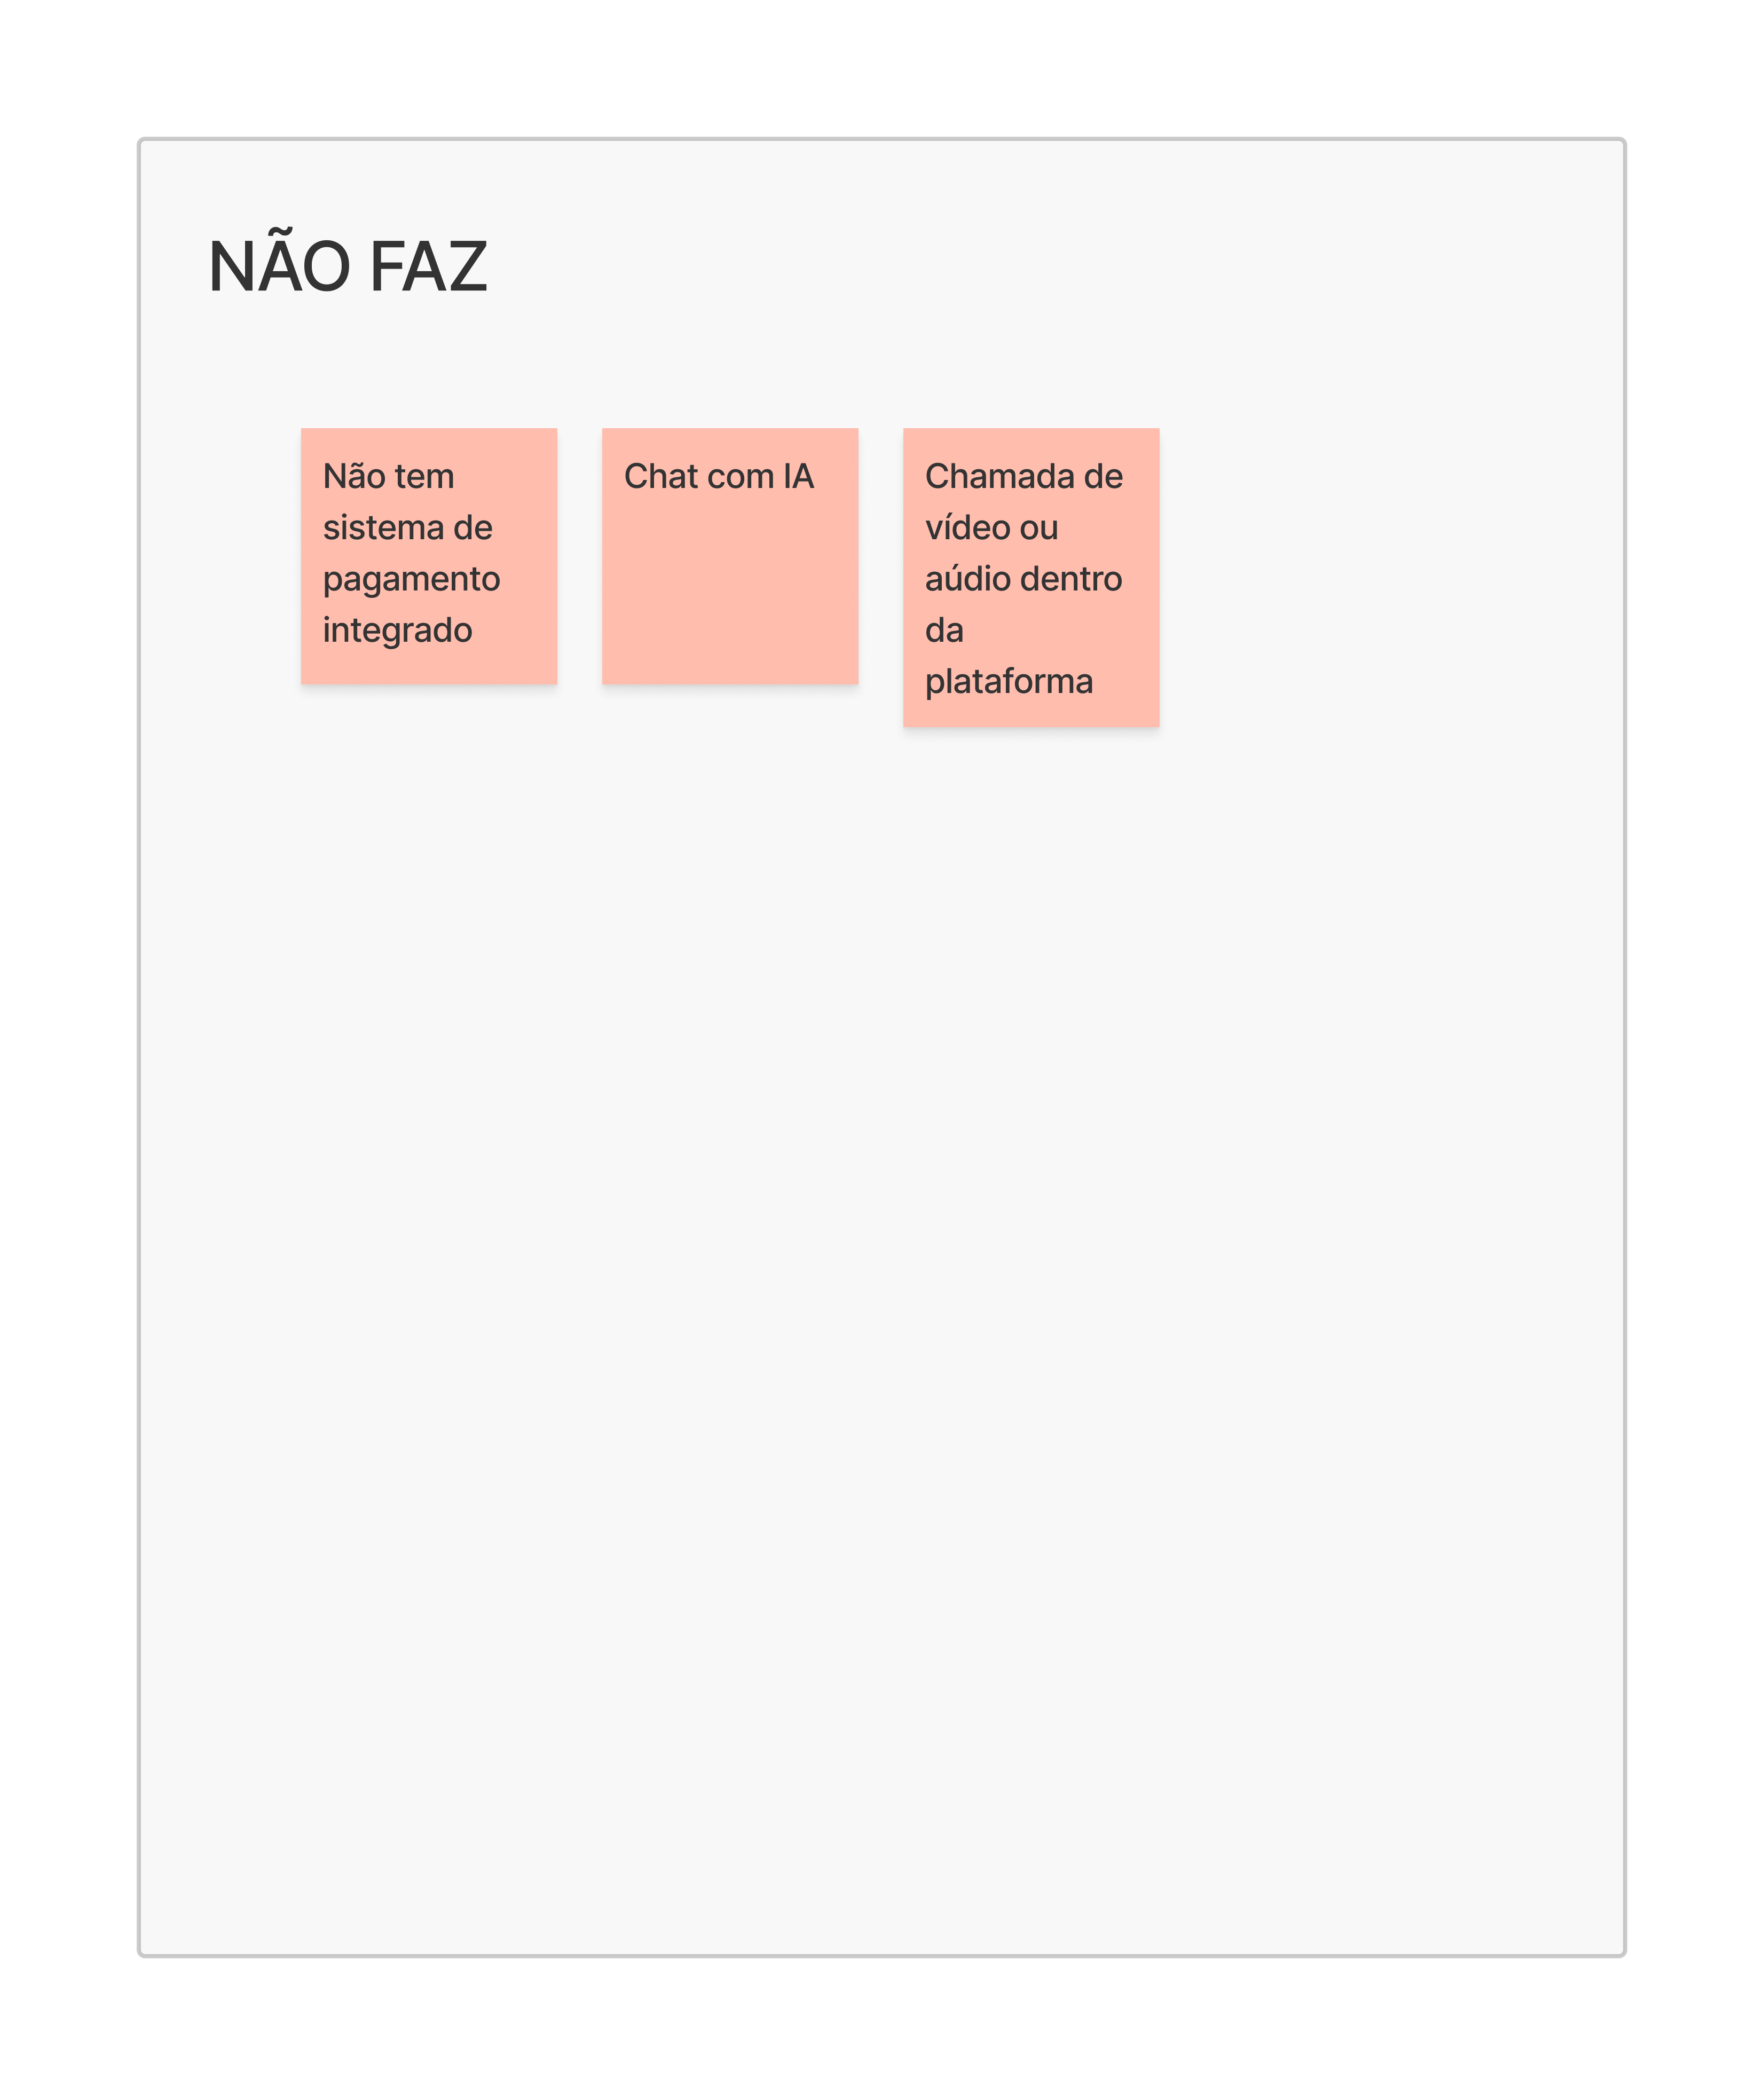
\includegraphics[width=0.9\textwidth]{figuras/Lean02NaoFaz.png}

    Fonte: Adaptado a partir de caroli.org

    \vspace{0.2cm}
\end{figure}

\begin{figure}[h!]
    \centering
    \caption{Objetivos do Produto.} 
    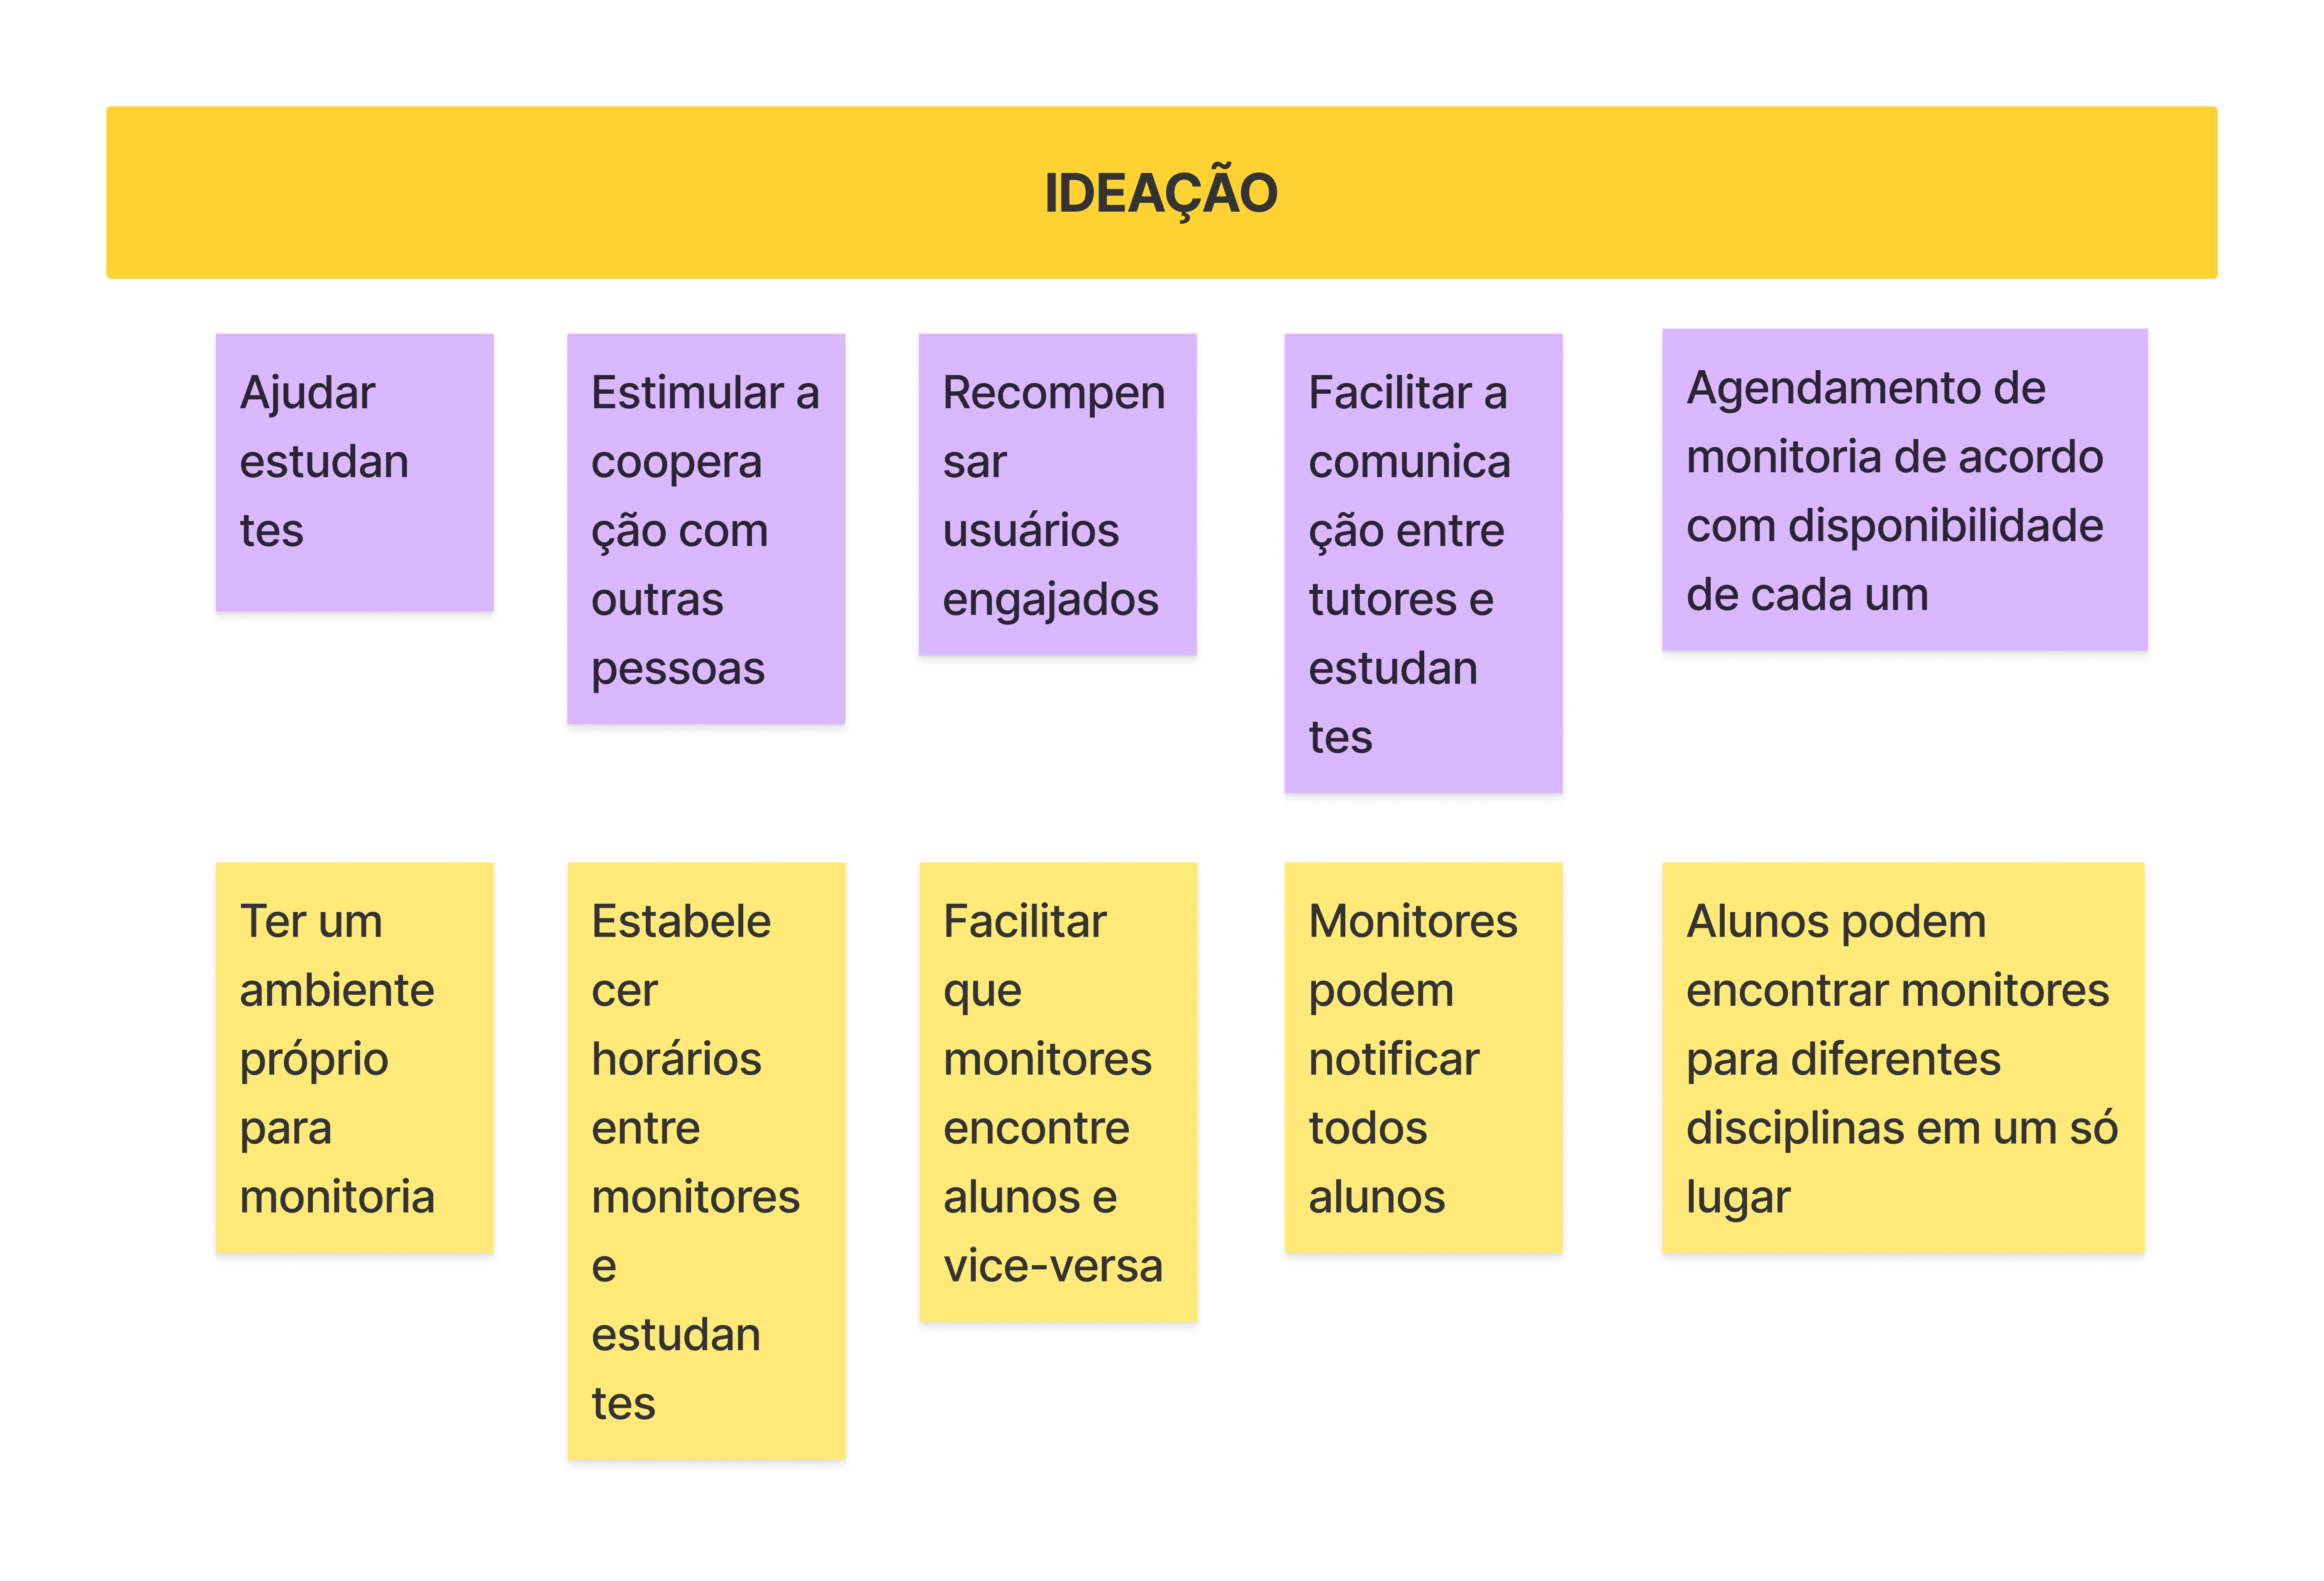
\includegraphics[width=0.9\textwidth]{figuras/Lean03Ideacao.png}

    Fonte: Adaptado a partir de caroli.org
    
    \vspace{0.2cm}
\end{figure}

\begin{figure}[h!]
    \centering
    \caption{Ideias de funcionalidades (Gamificação, Comunicação, Recomendação).} 
    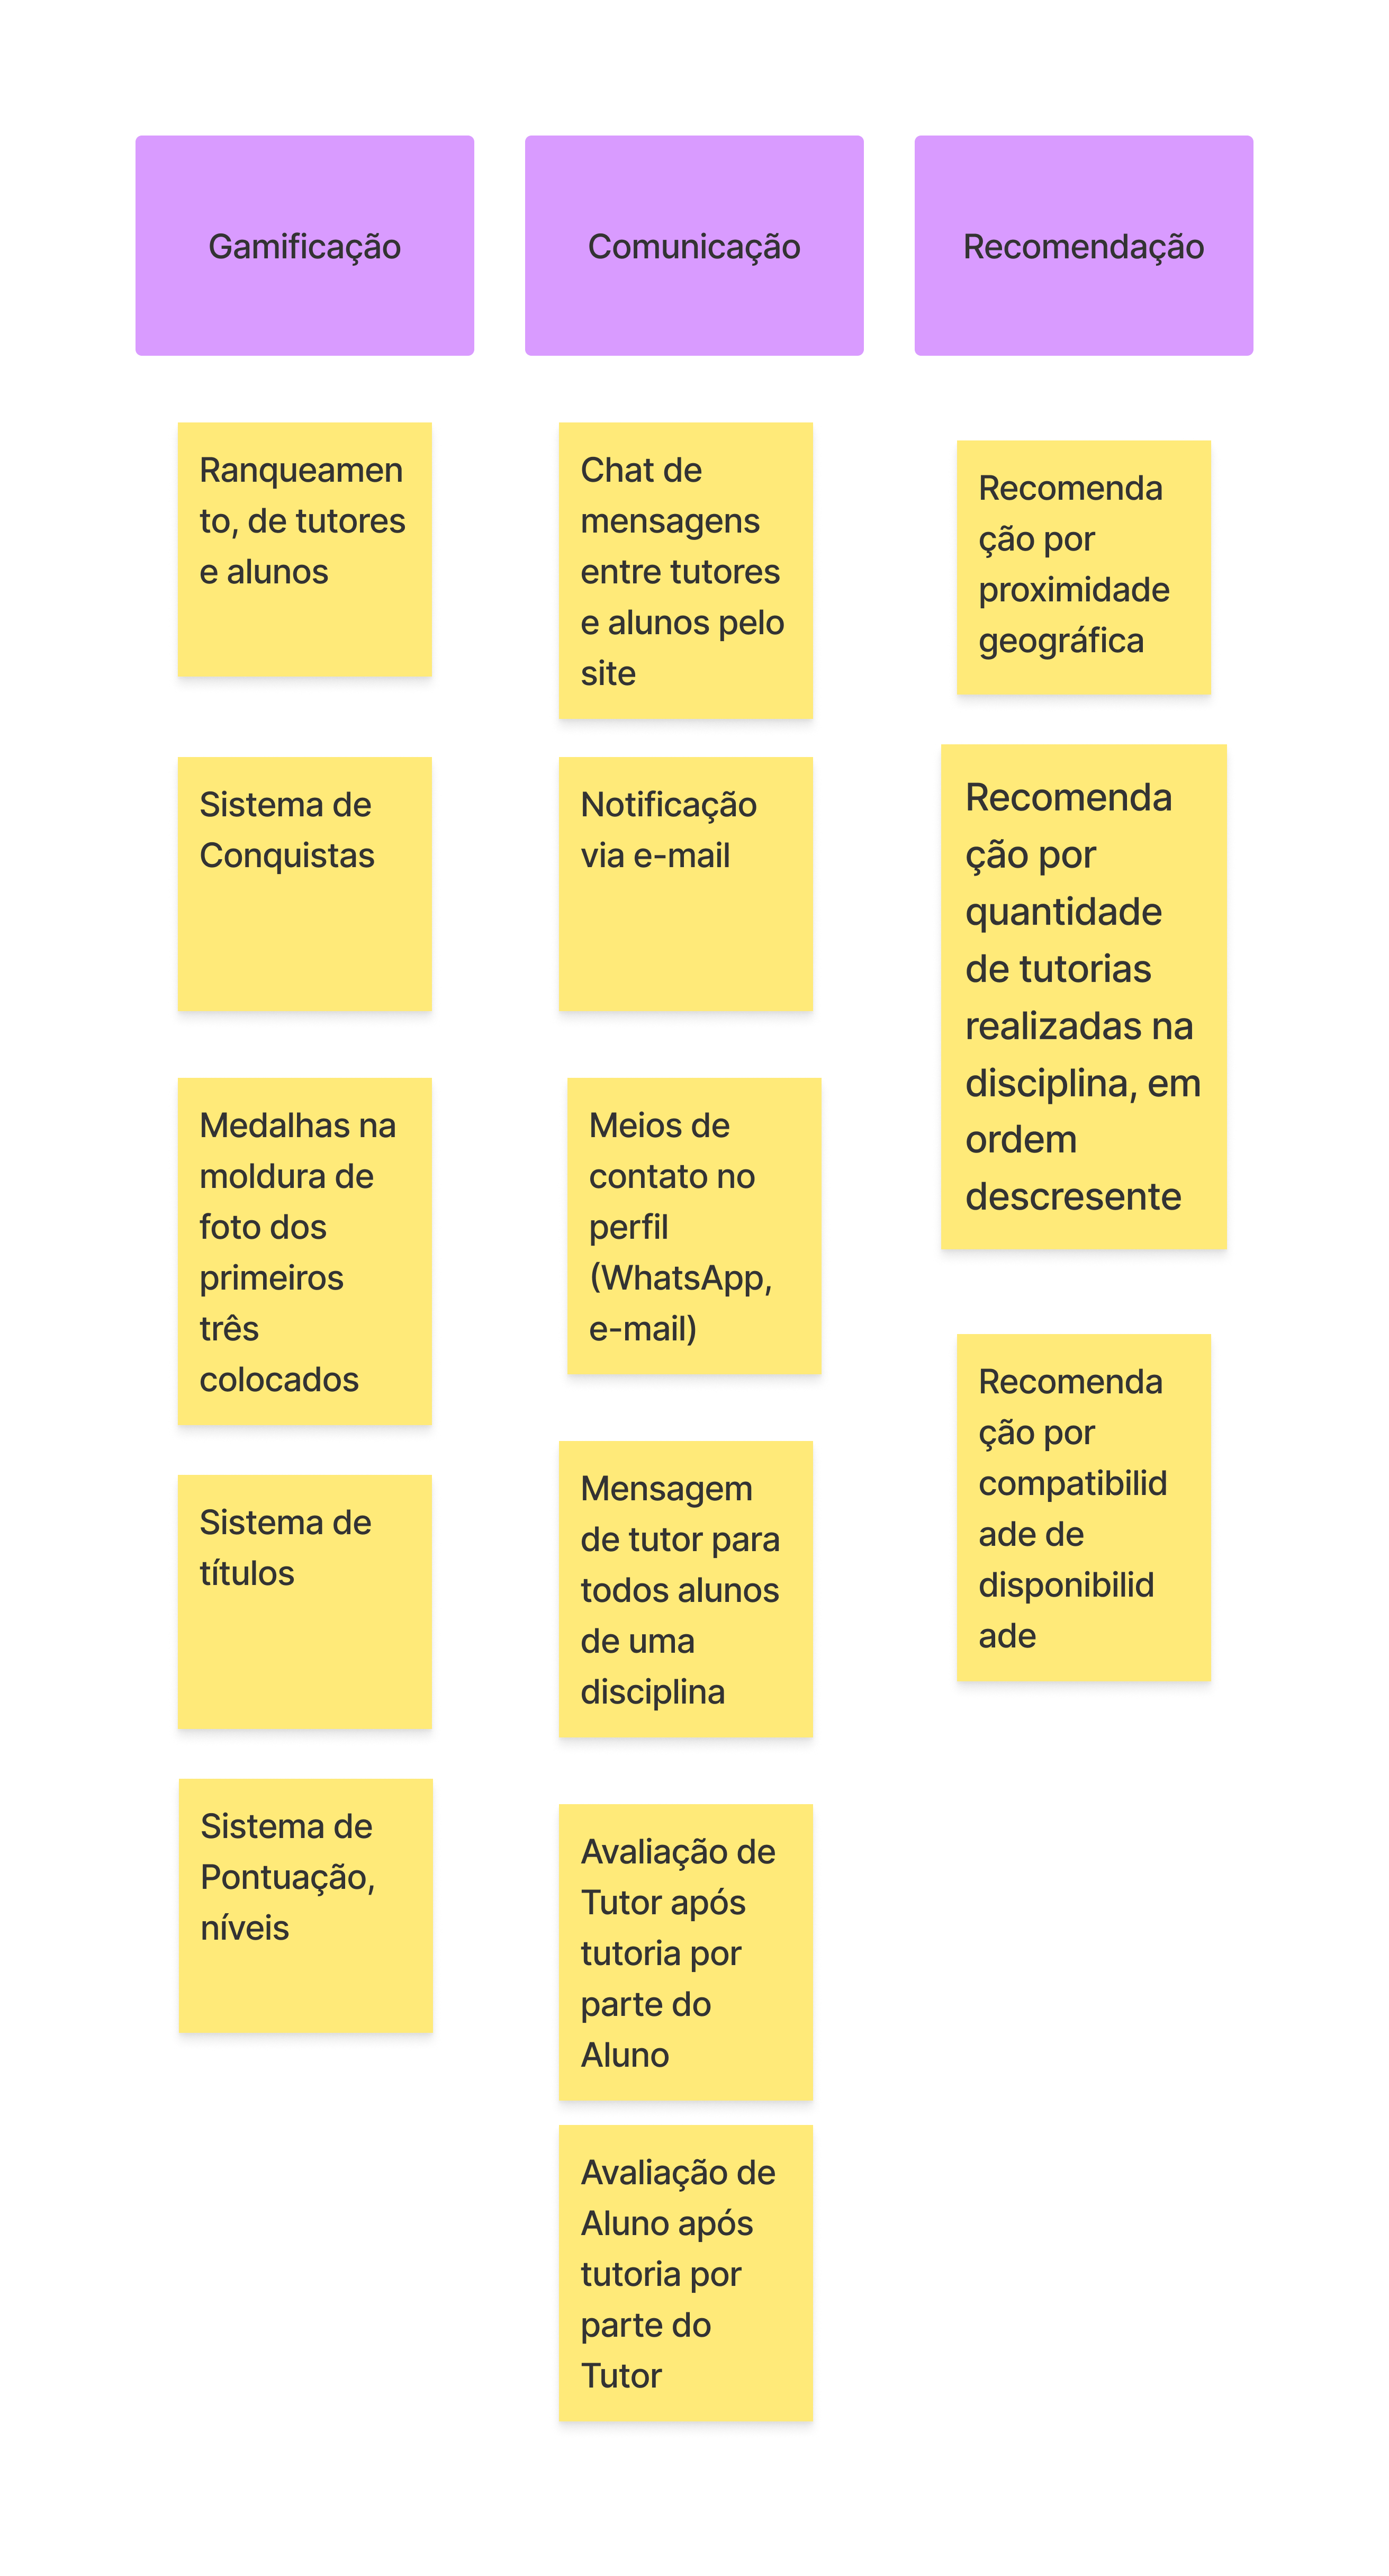
\includegraphics[width=0.7\textwidth]{figuras/Lean03Ideacao2.png}

    Fonte: Adaptado a partir de caroli.org
    
    \vspace{0.2cm}
\end{figure}

\begin{figure}[h!]
    \centering
    \caption{Ideias de funcionalidades (CRUDs).} 
    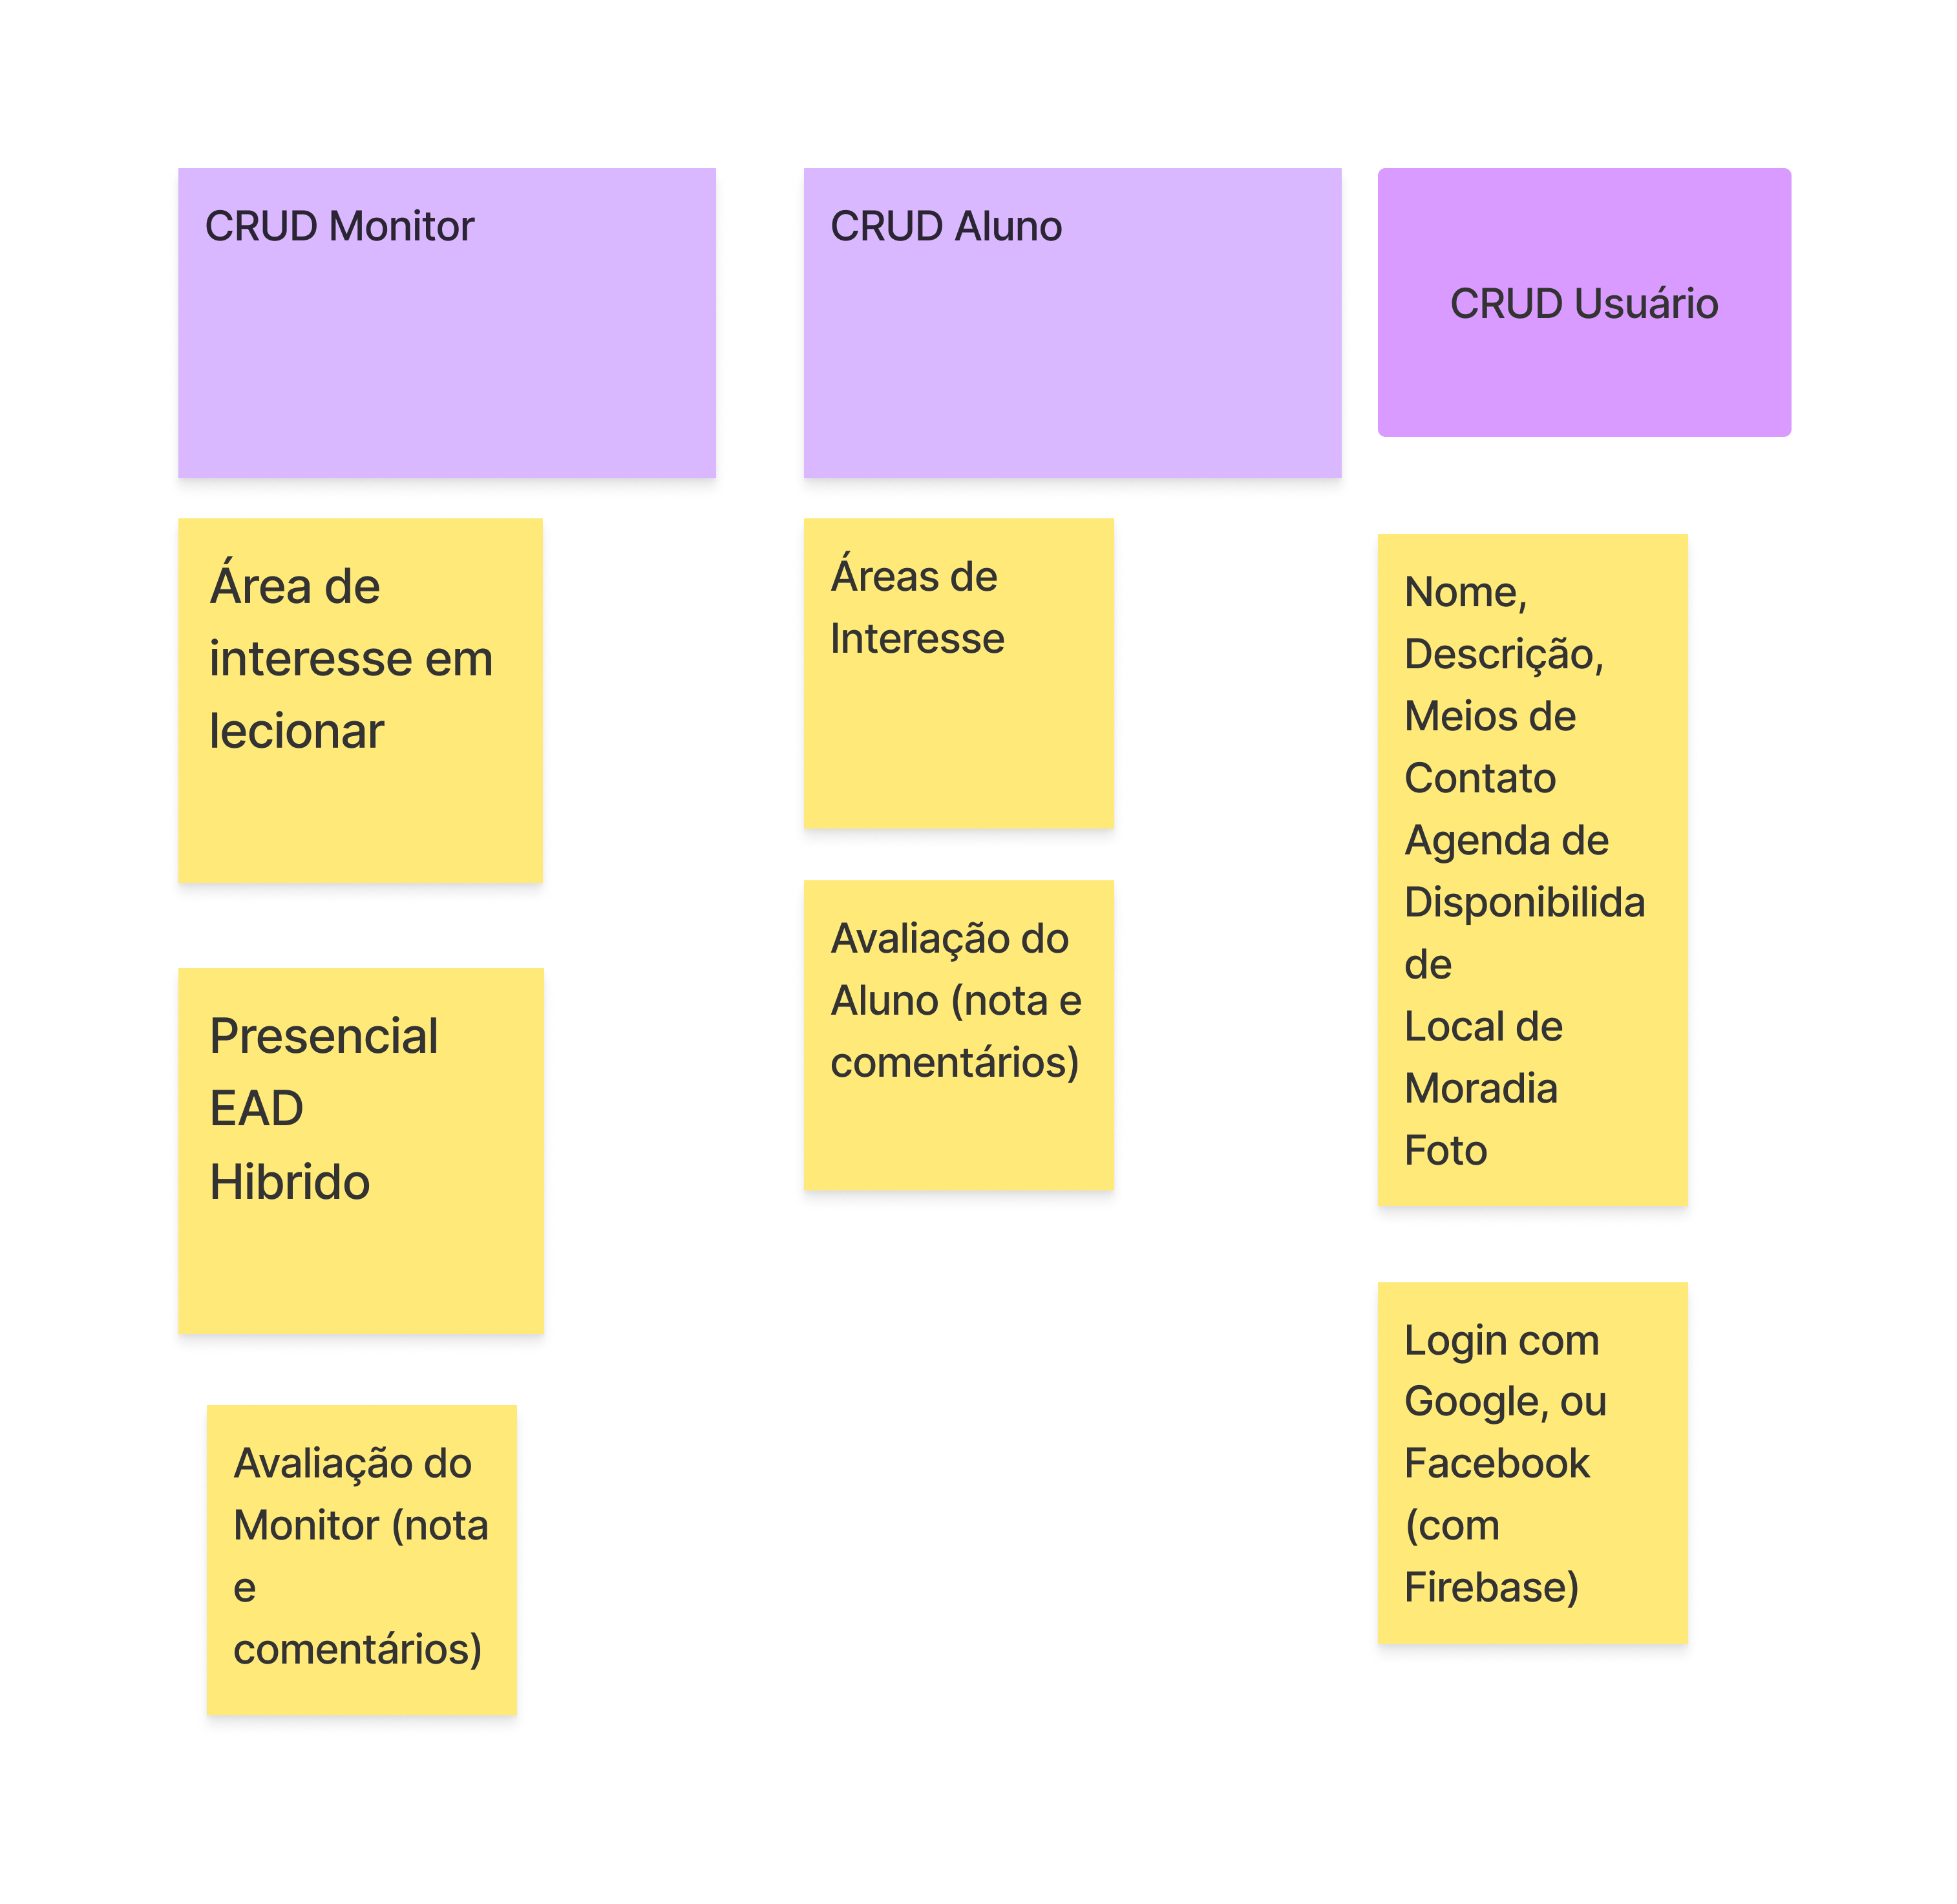
\includegraphics[width=0.9\textwidth]{figuras/Lean03Ideacao3.png}
    

    Fonte: Adaptado a partir de caroli.org
    
    \vspace{0.2cm}
\end{figure}

\begin{figure}[h!]
    \centering
    \caption{Persona do Aprendiz.} 
    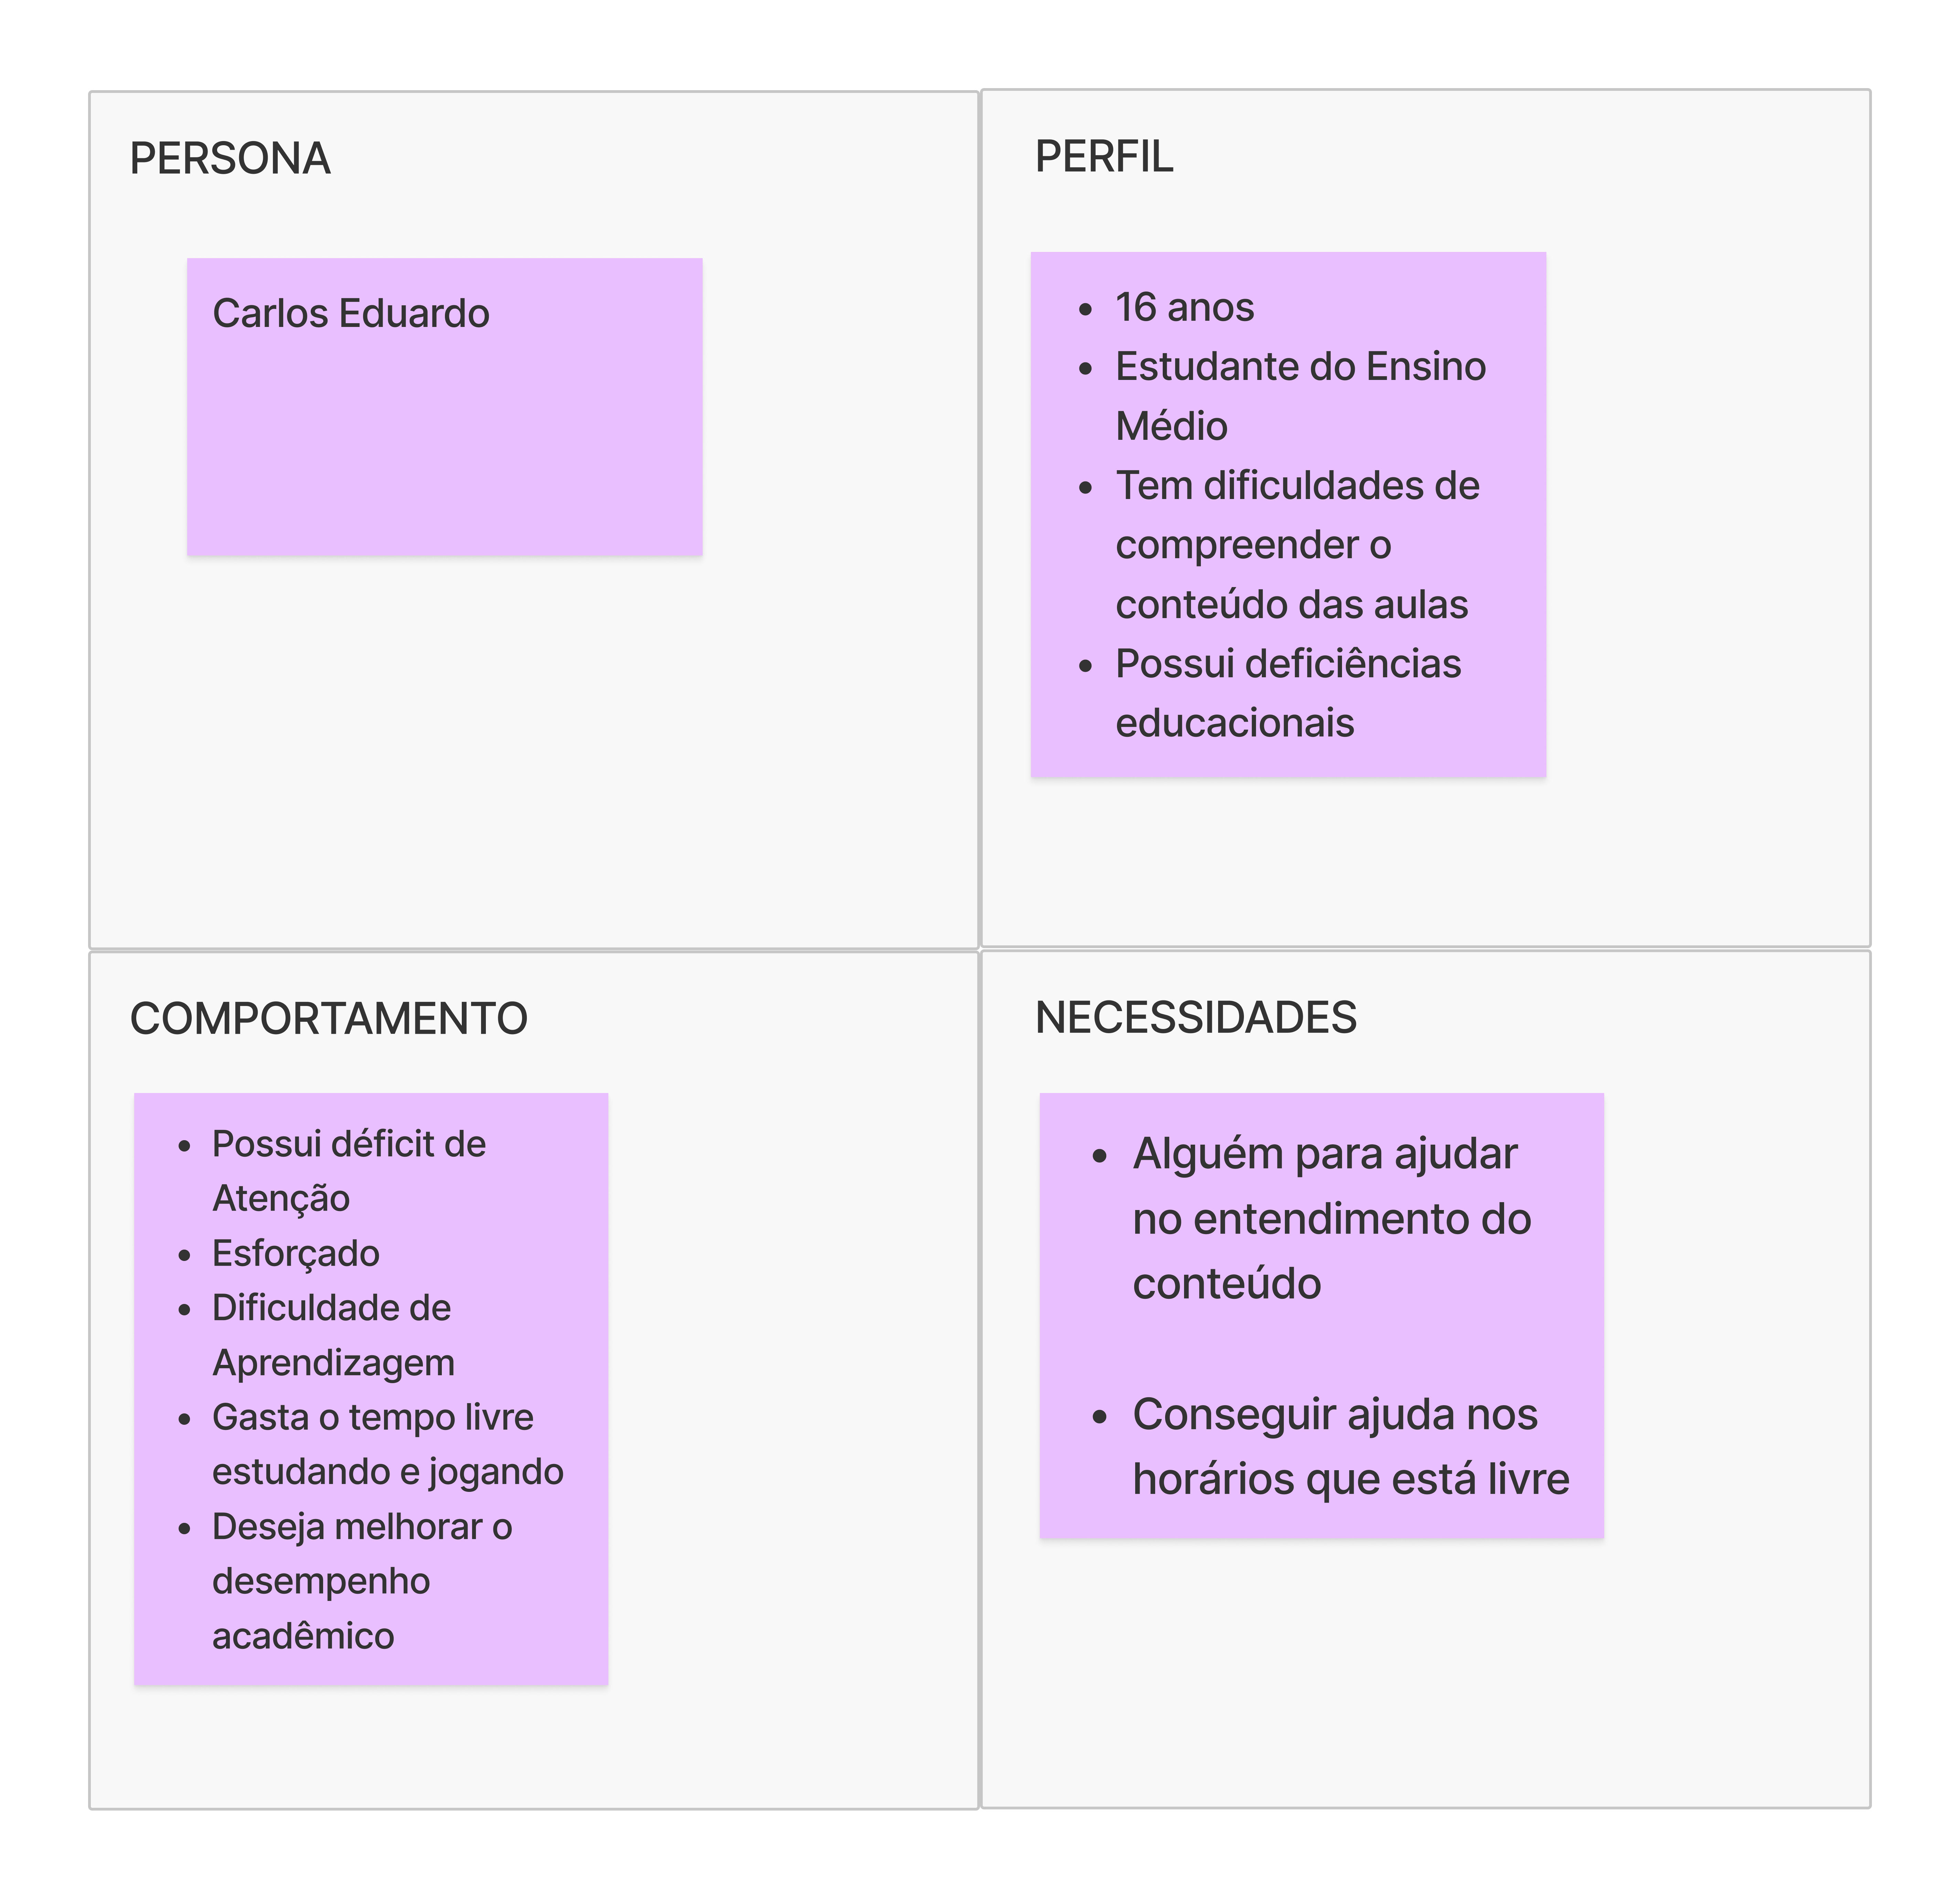
\includegraphics[width=0.9\textwidth]{figuras/Lean04Persona1.png}

    Fonte: Adaptado a partir de caroli.org
    
    \vspace{0.2cm}
\end{figure}

\begin{figure}[h!]
    \centering
    \caption{Persona do Tutor.} 
    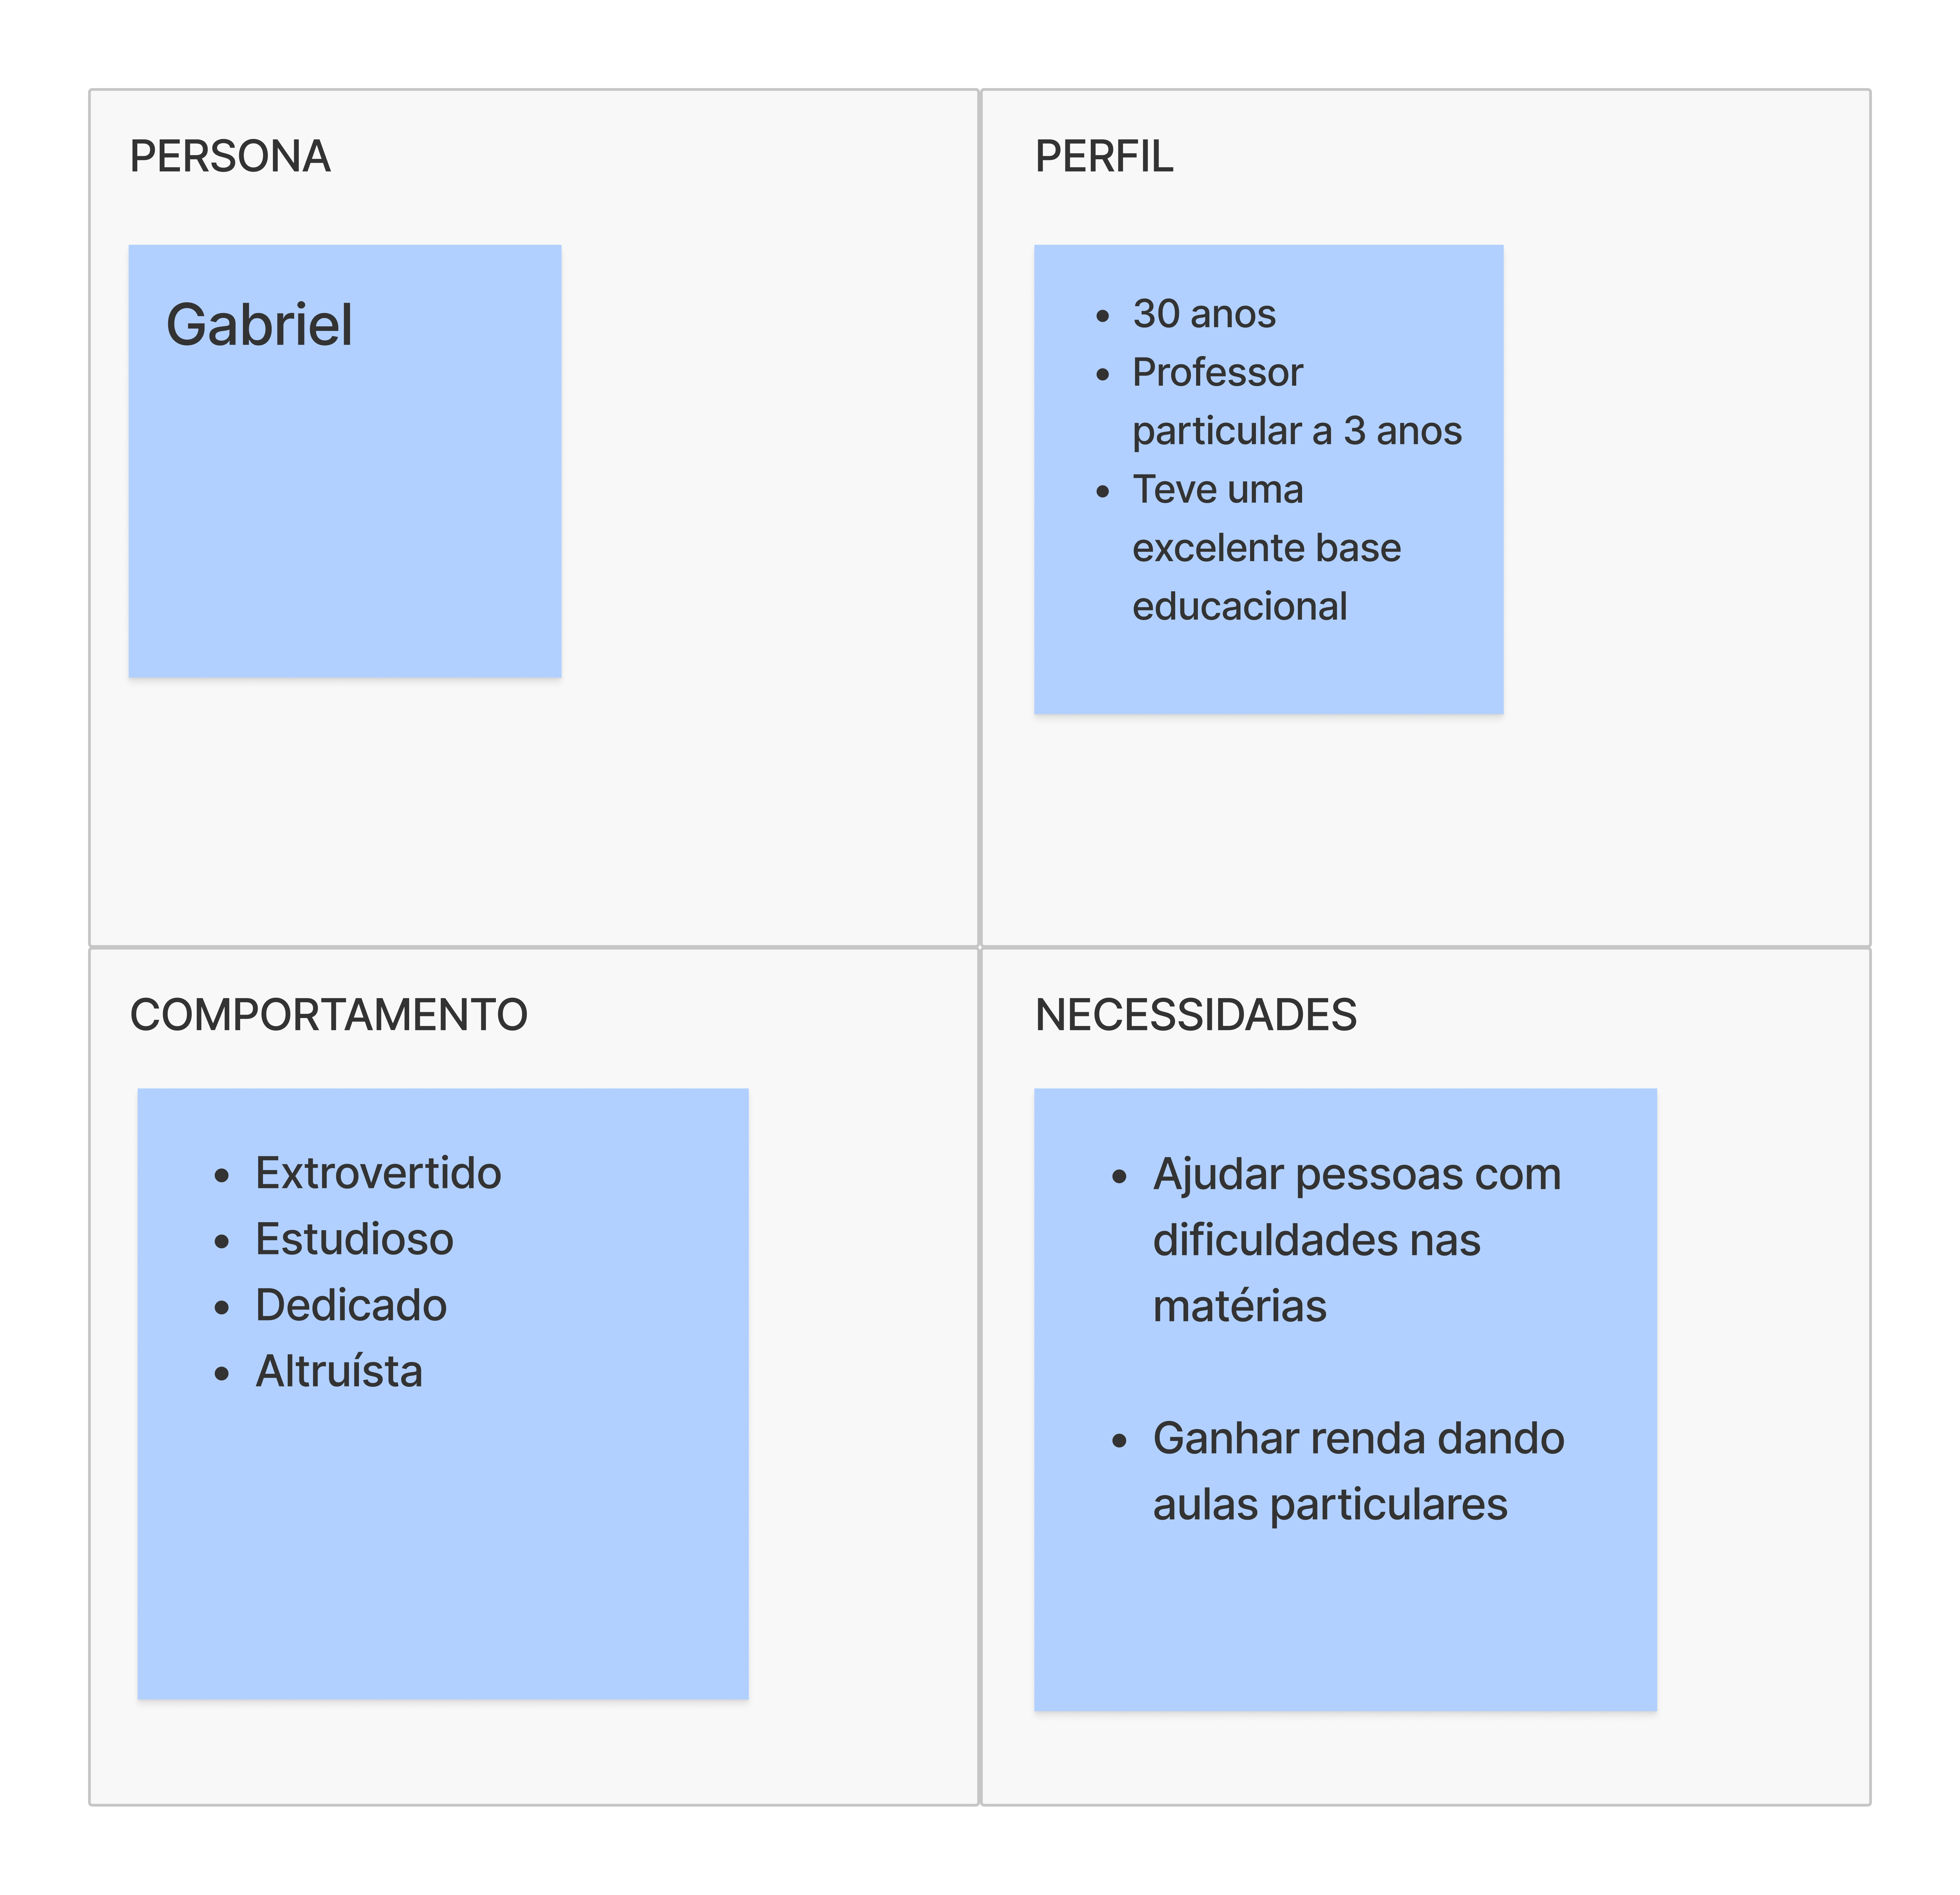
\includegraphics[width=0.9\textwidth]{figuras/Lean05Persona2.png}

    Fonte: Adaptado a partir de caroli.org
    
    \vspace{0.2cm}
\end{figure}

% \begin{figure}[h!]
%     \centering
%     \caption{Persona 3.} 
%     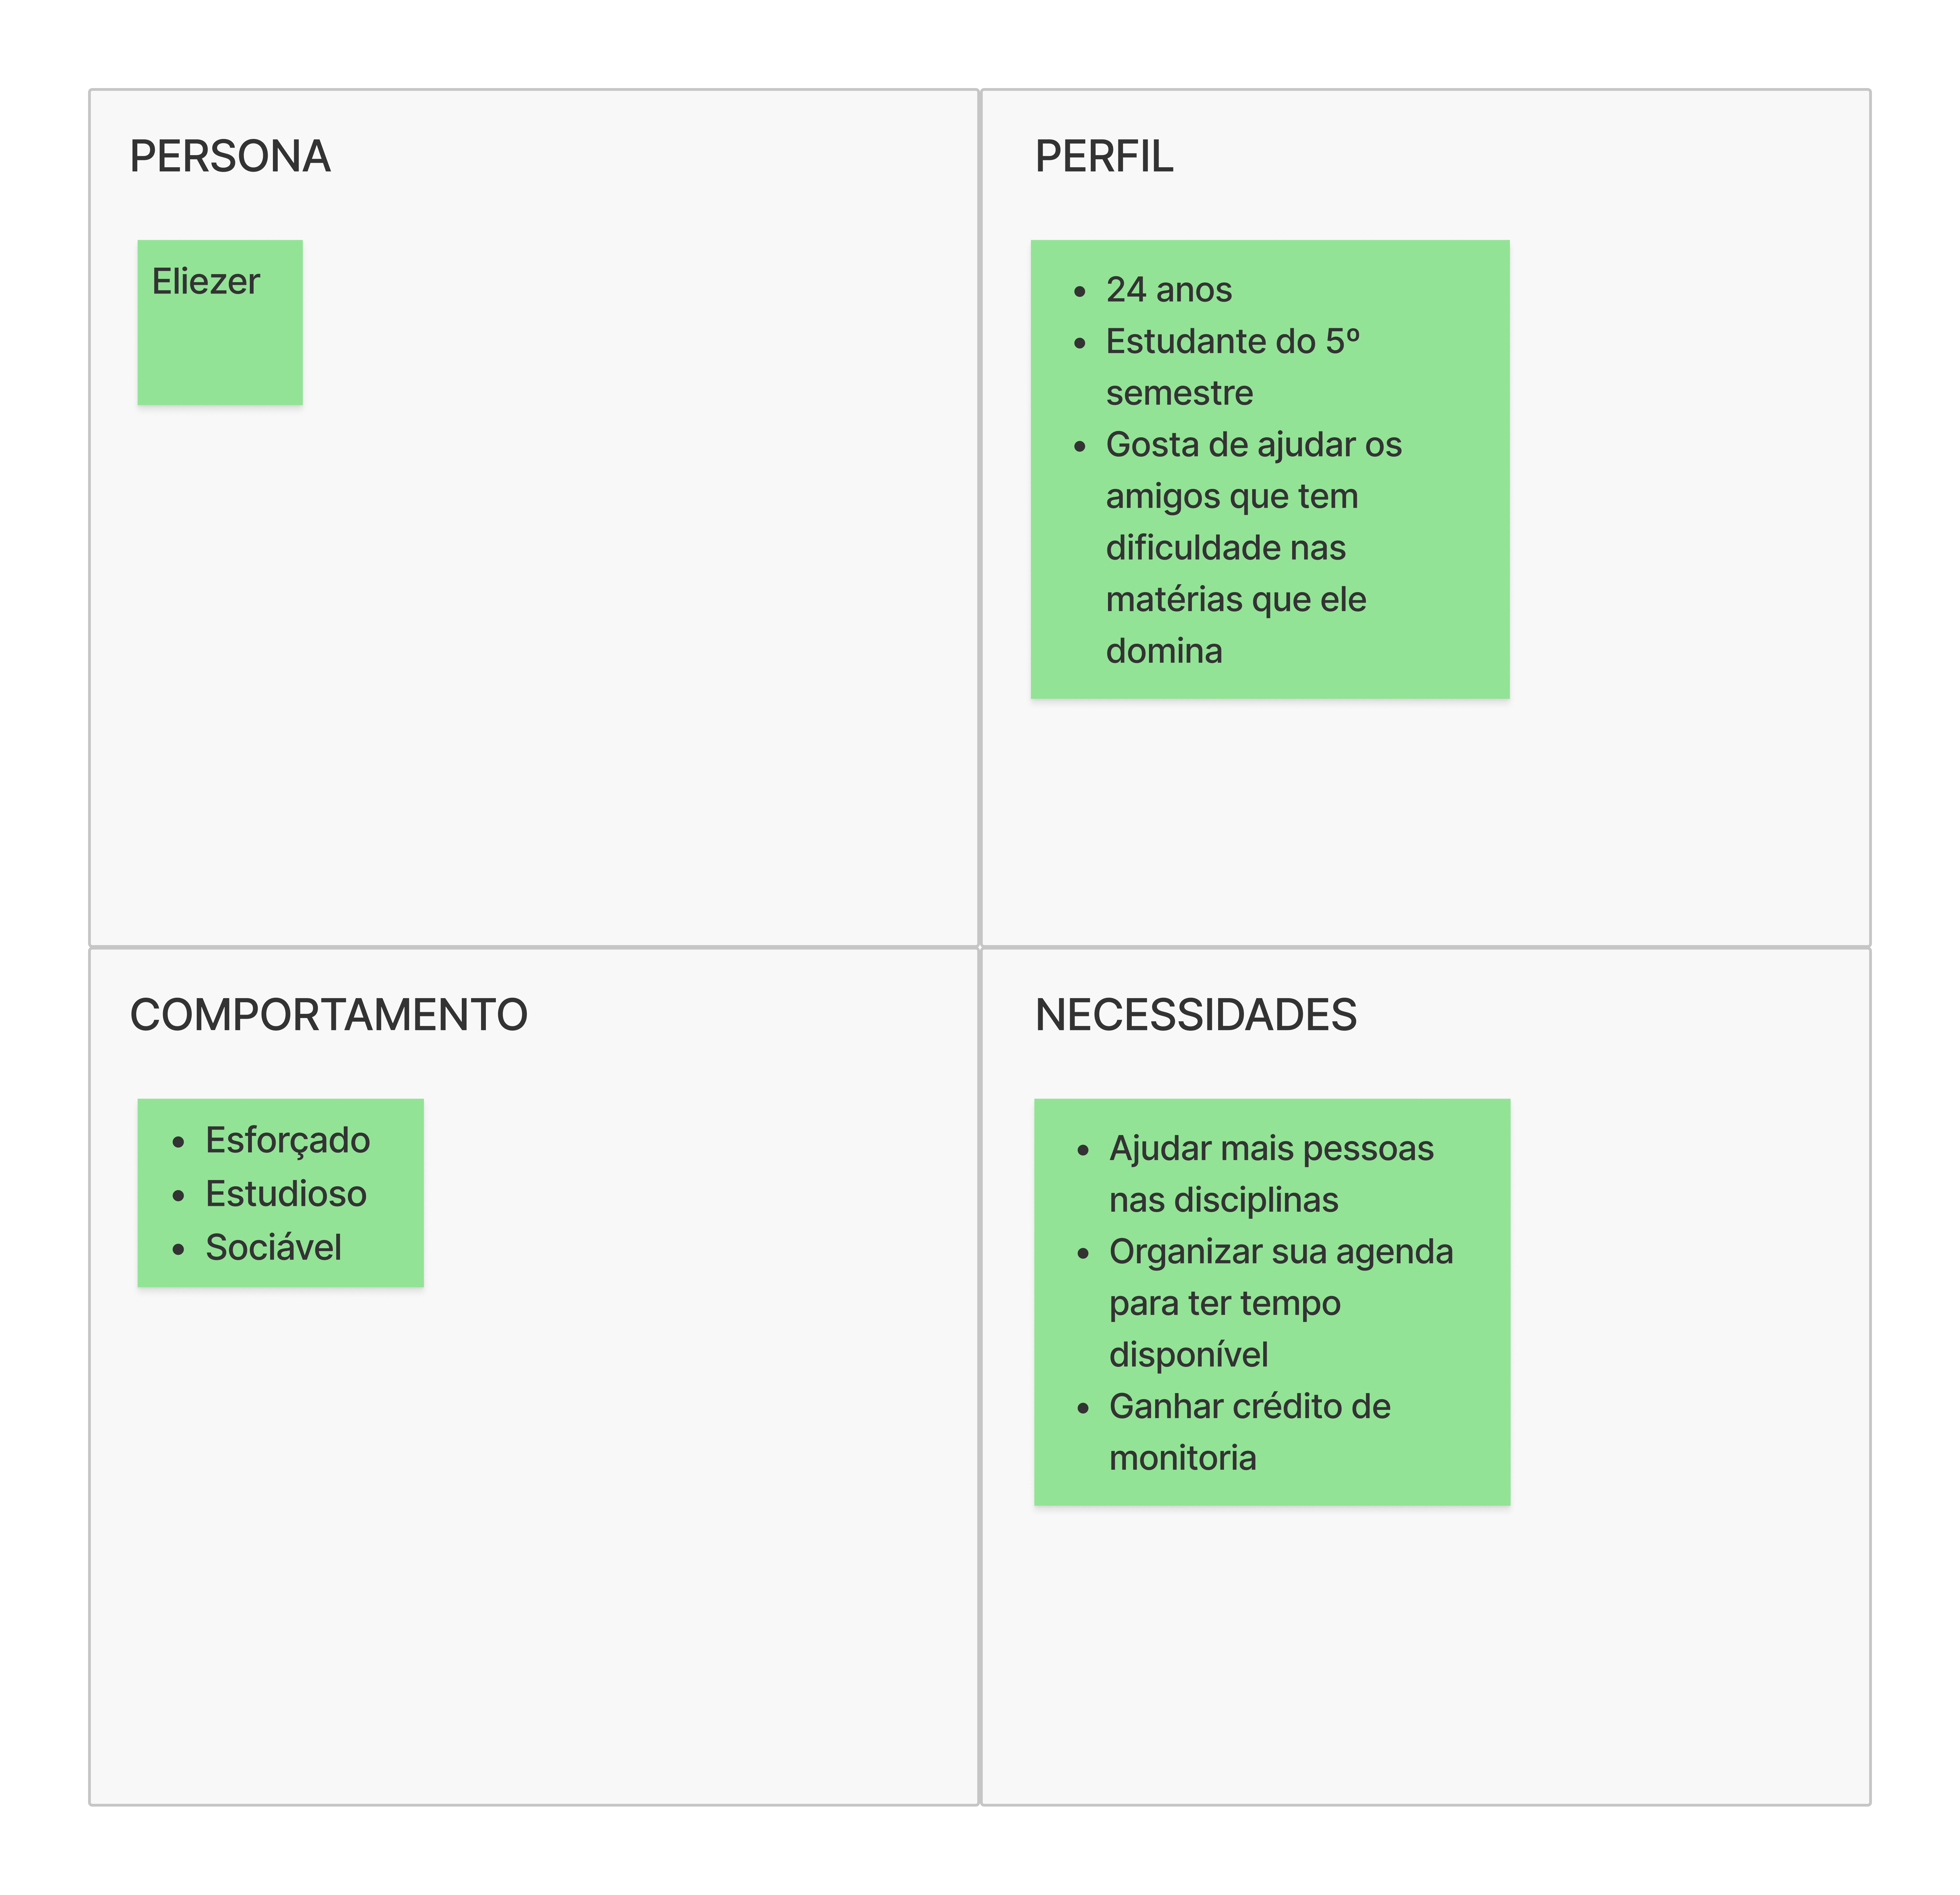
\includegraphics[width=0.9\textwidth]{figuras/Lean06Persona3.png}

%     Fonte: Adaptada a partir de caroli.org
    
%     \vspace{0.2cm}
% \end{figure}

% \begin{figure}[h!]
%     \centering
%     \caption{Persona 1.} 
%     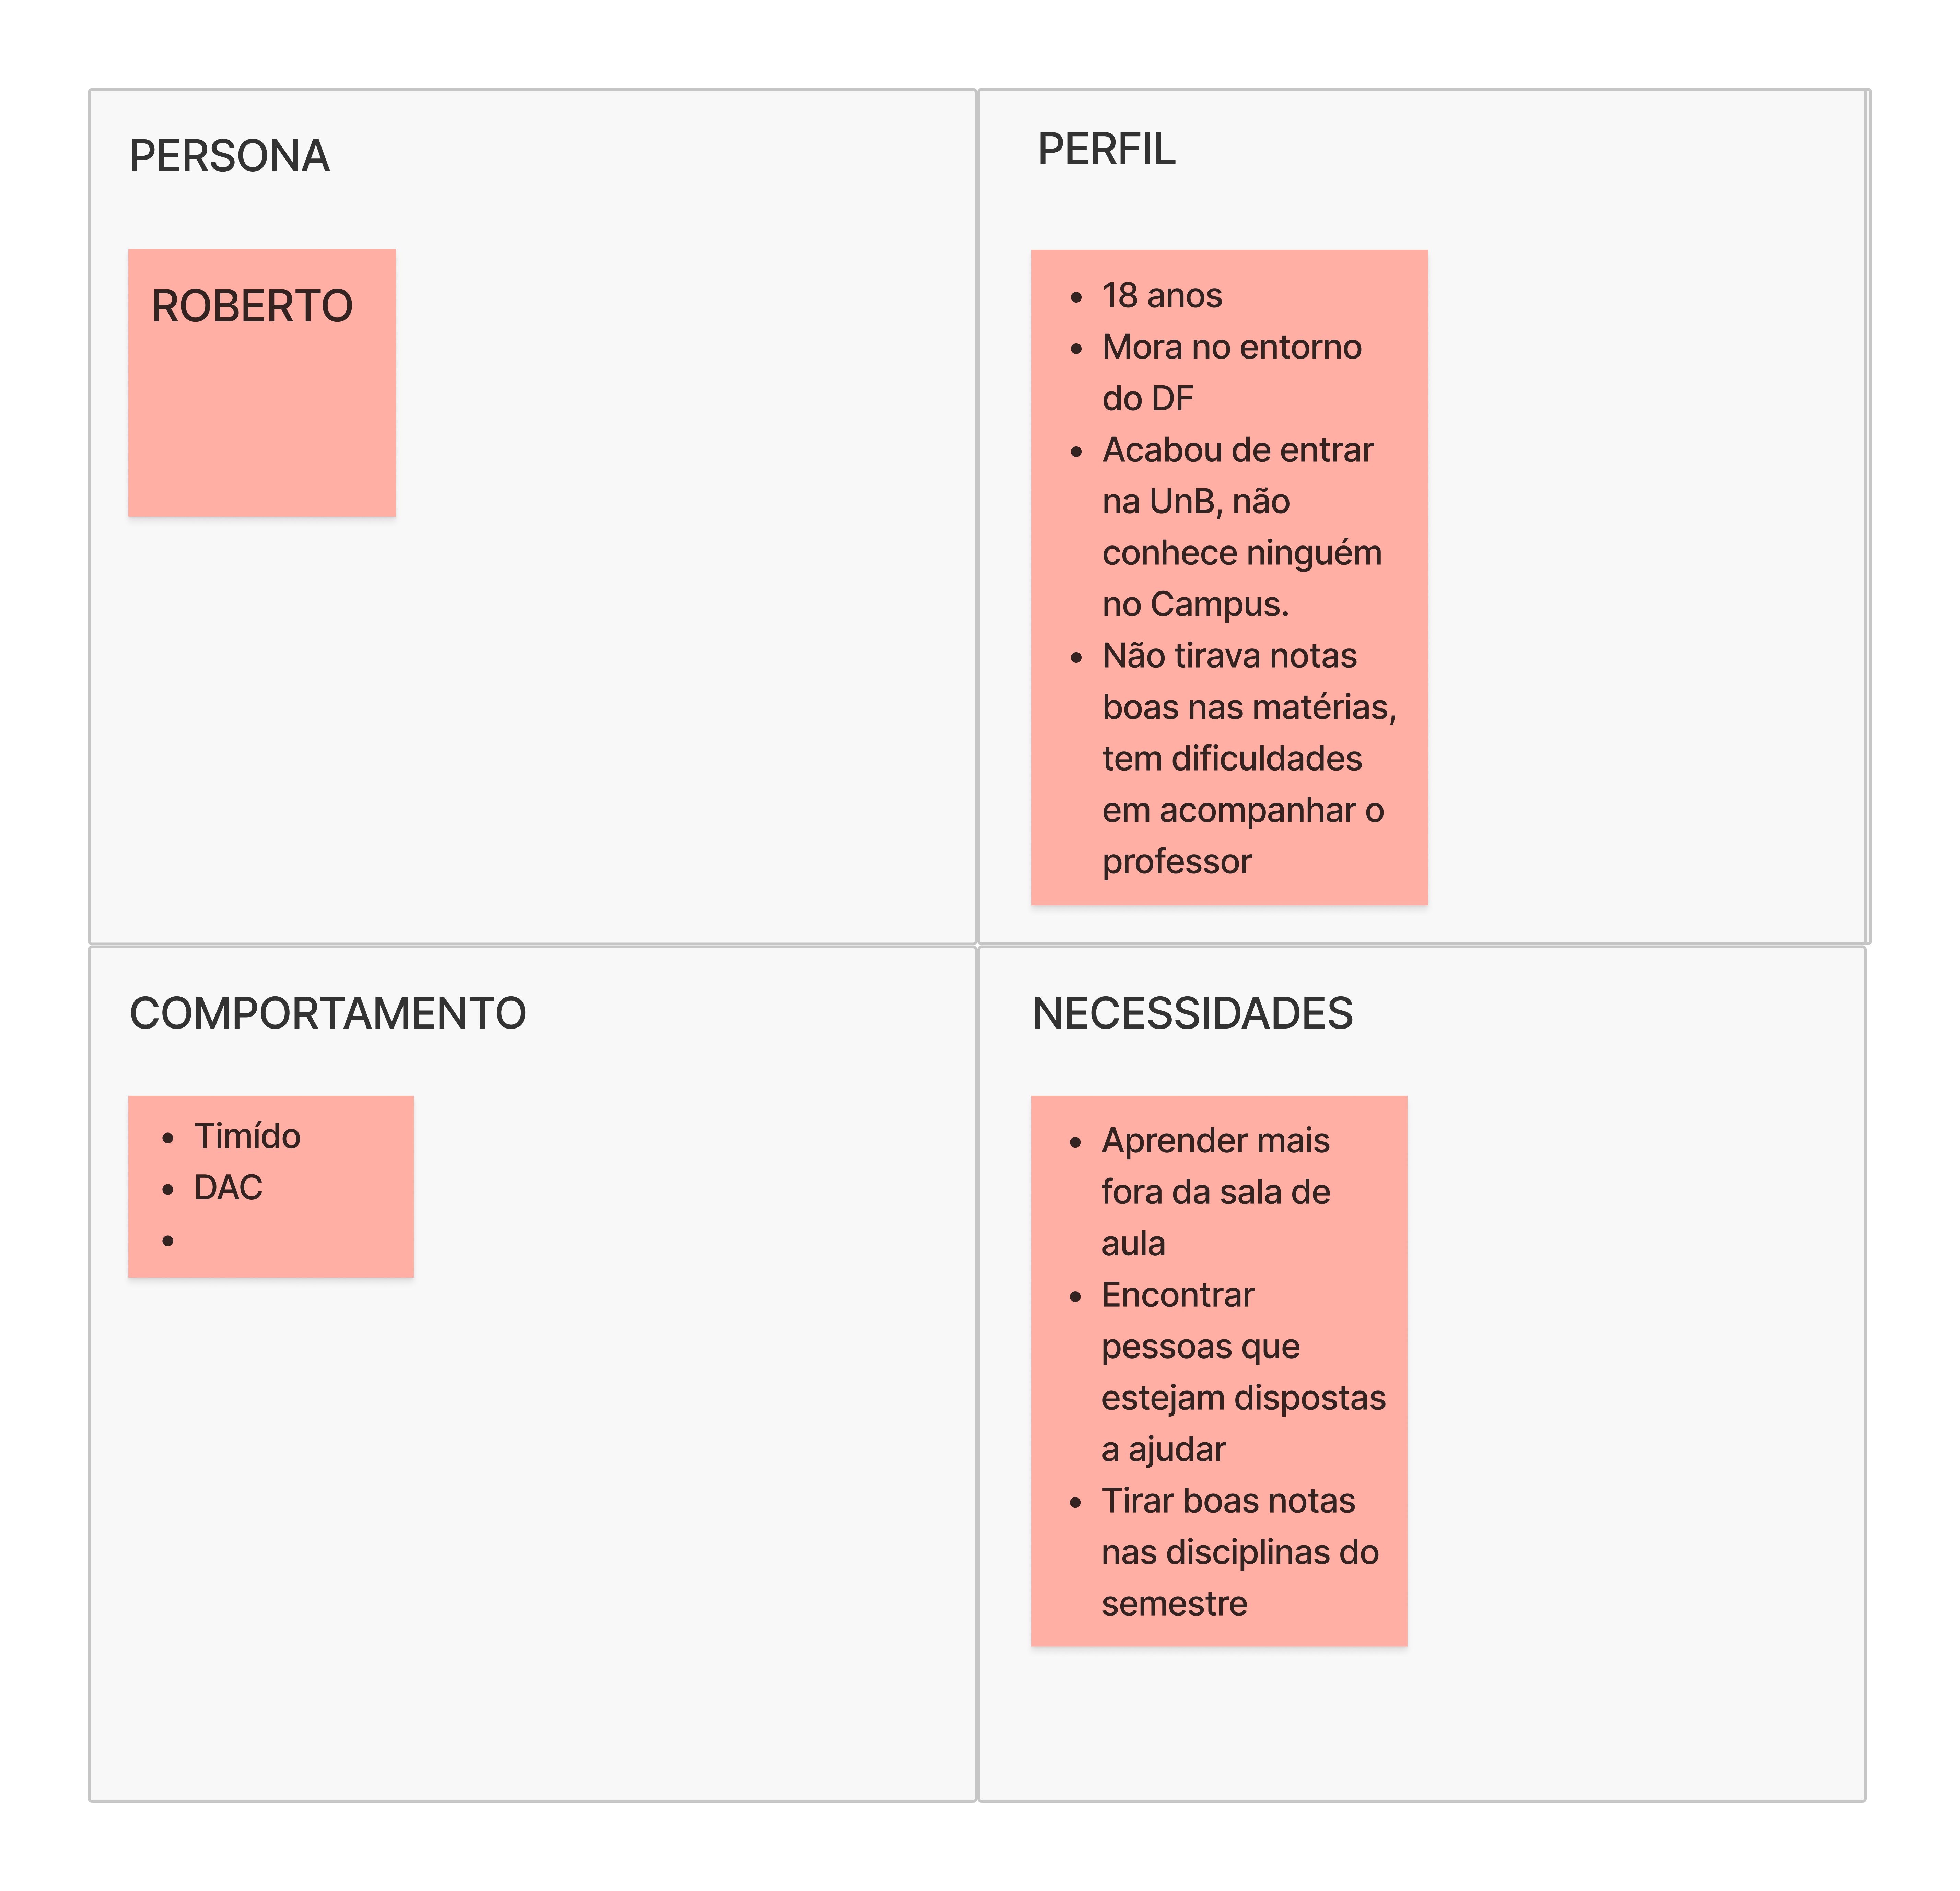
\includegraphics[width=0.9\textwidth]{figuras/Lean07Persona4.png}

%     Fonte: Adaptada a partir de caroli.org
    
%     \vspace{0.2cm}
% \end{figure}

\begin{figure}[h!]
    \centering
    \caption{Jornada do Aprendiz.} 
    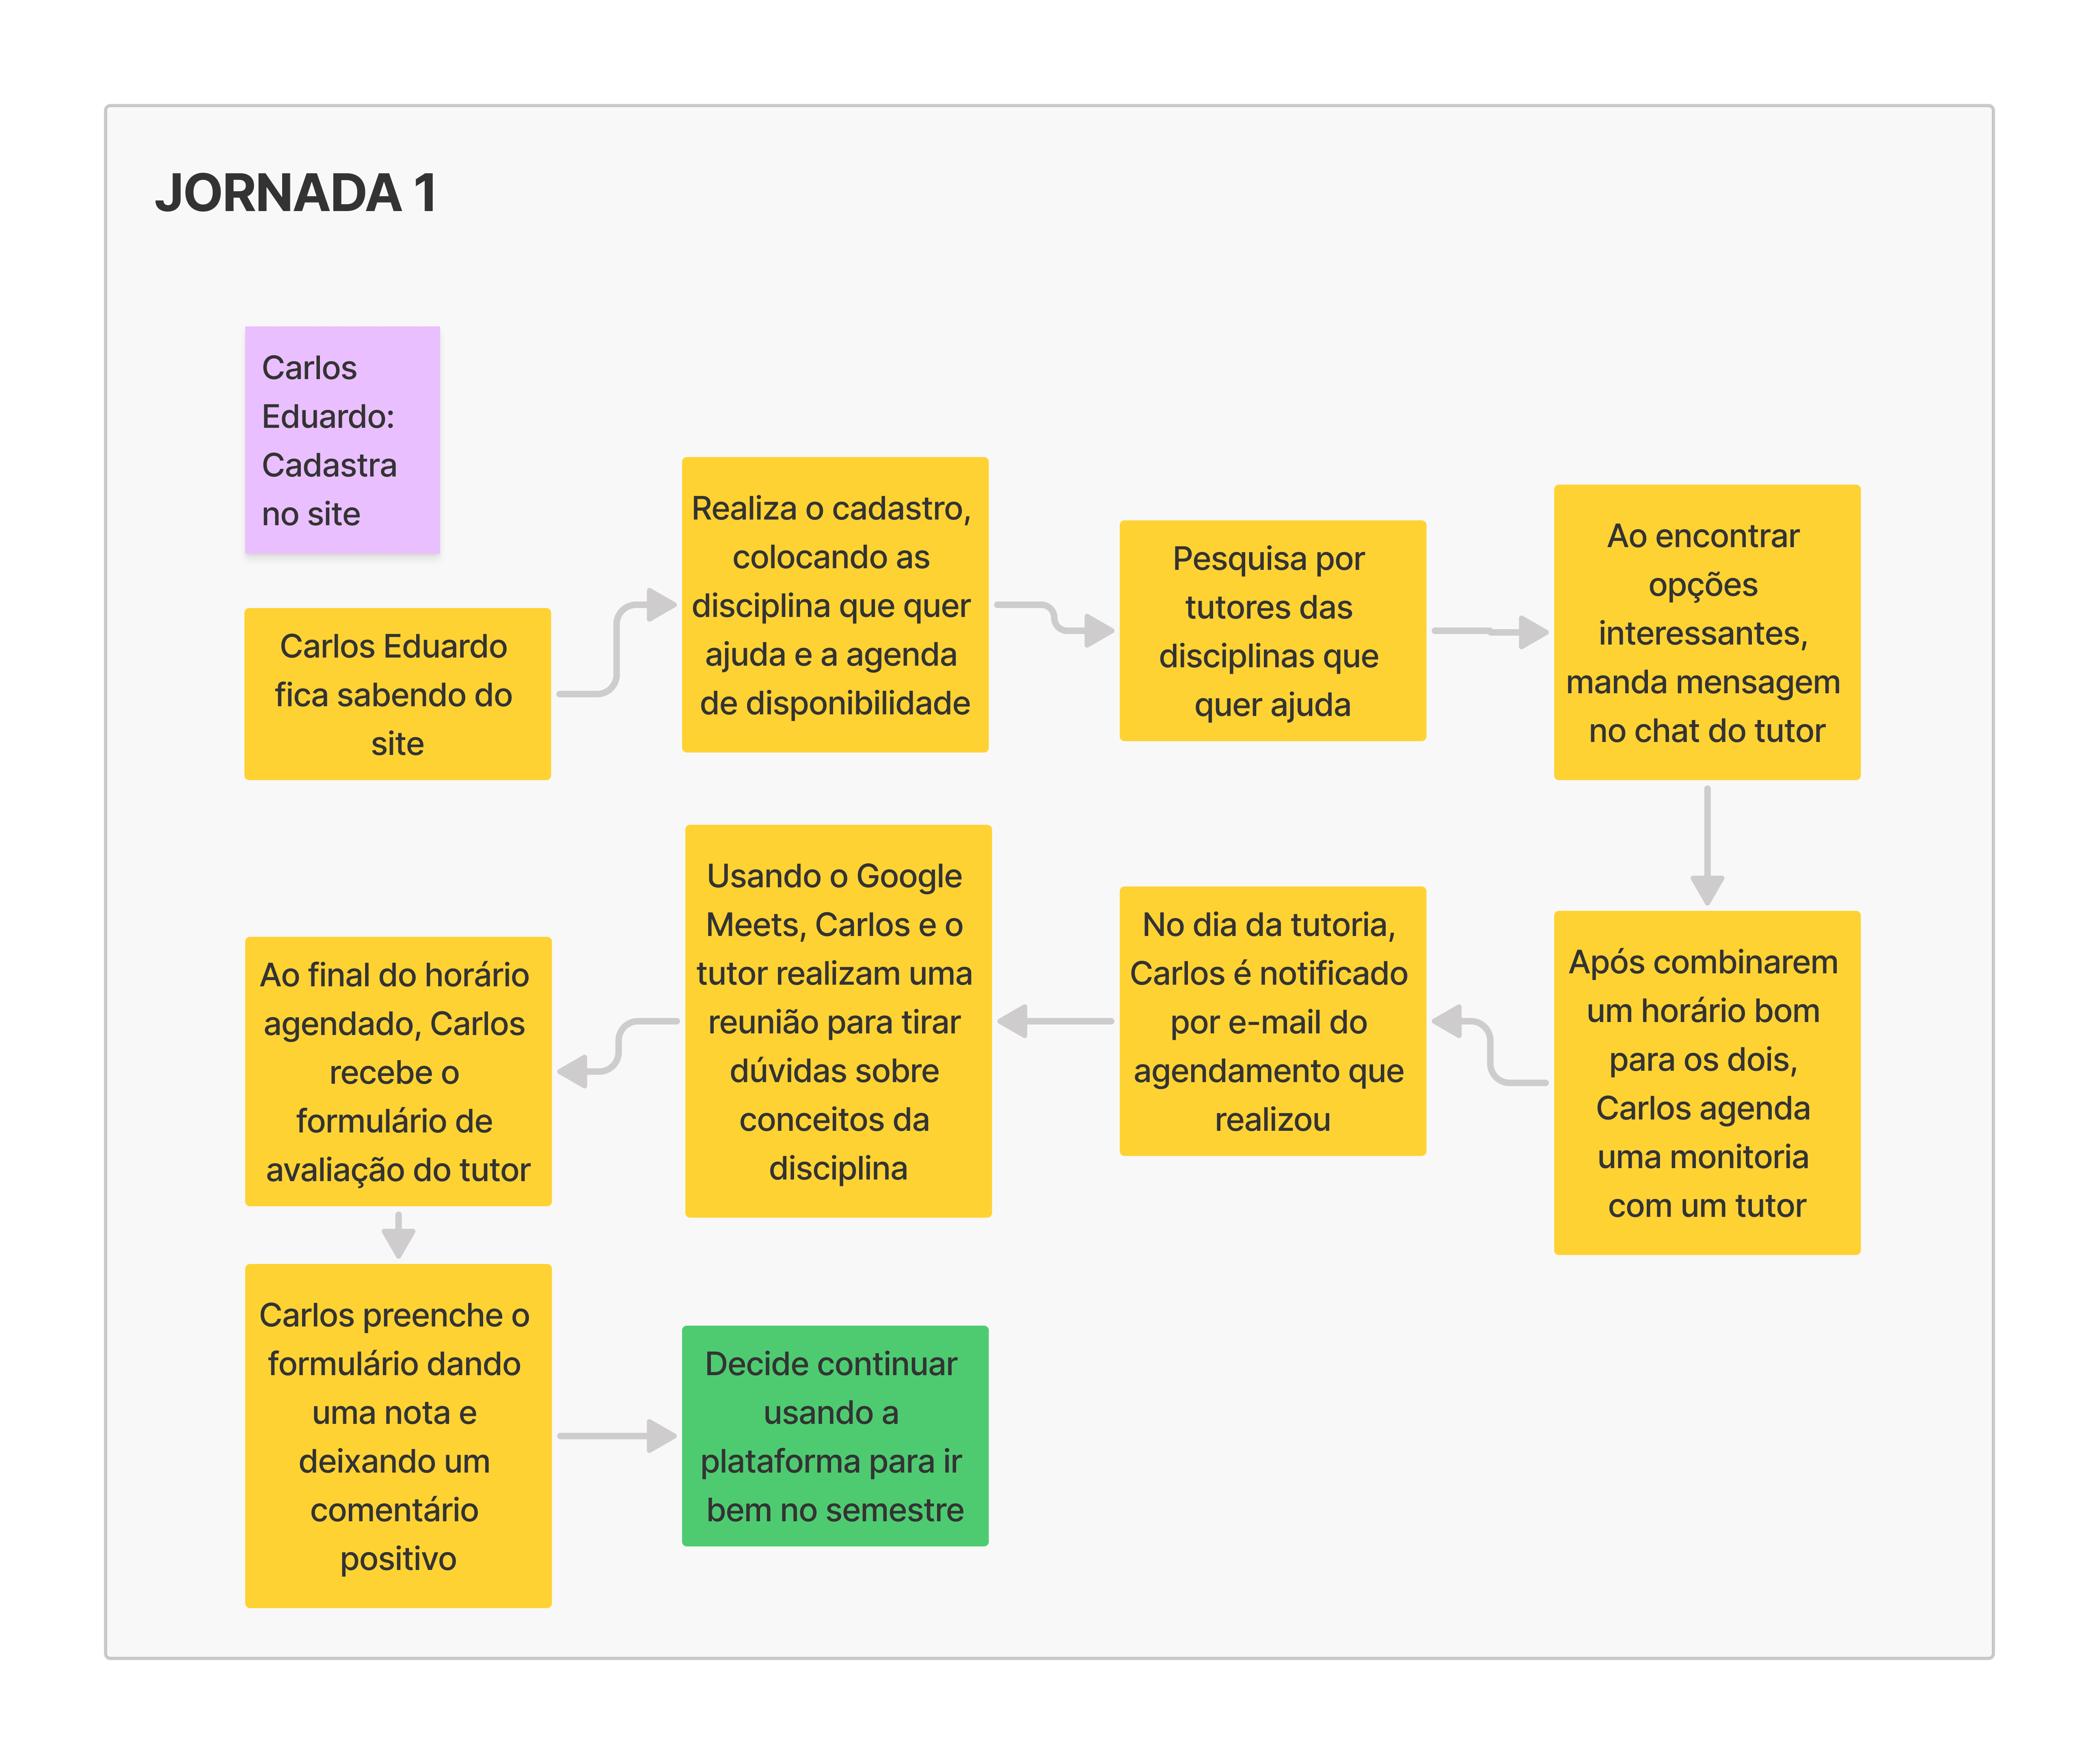
\includegraphics[width=1\textwidth]{figuras/Lean08Jornada1.png}

    Fonte: Adaptado a partir de caroli.org
    
    \vspace{0.2cm}
\end{figure}

\begin{figure}[h!]
    \centering
    \caption{\textit{Brainstorm} de Funcionalidades.} 
    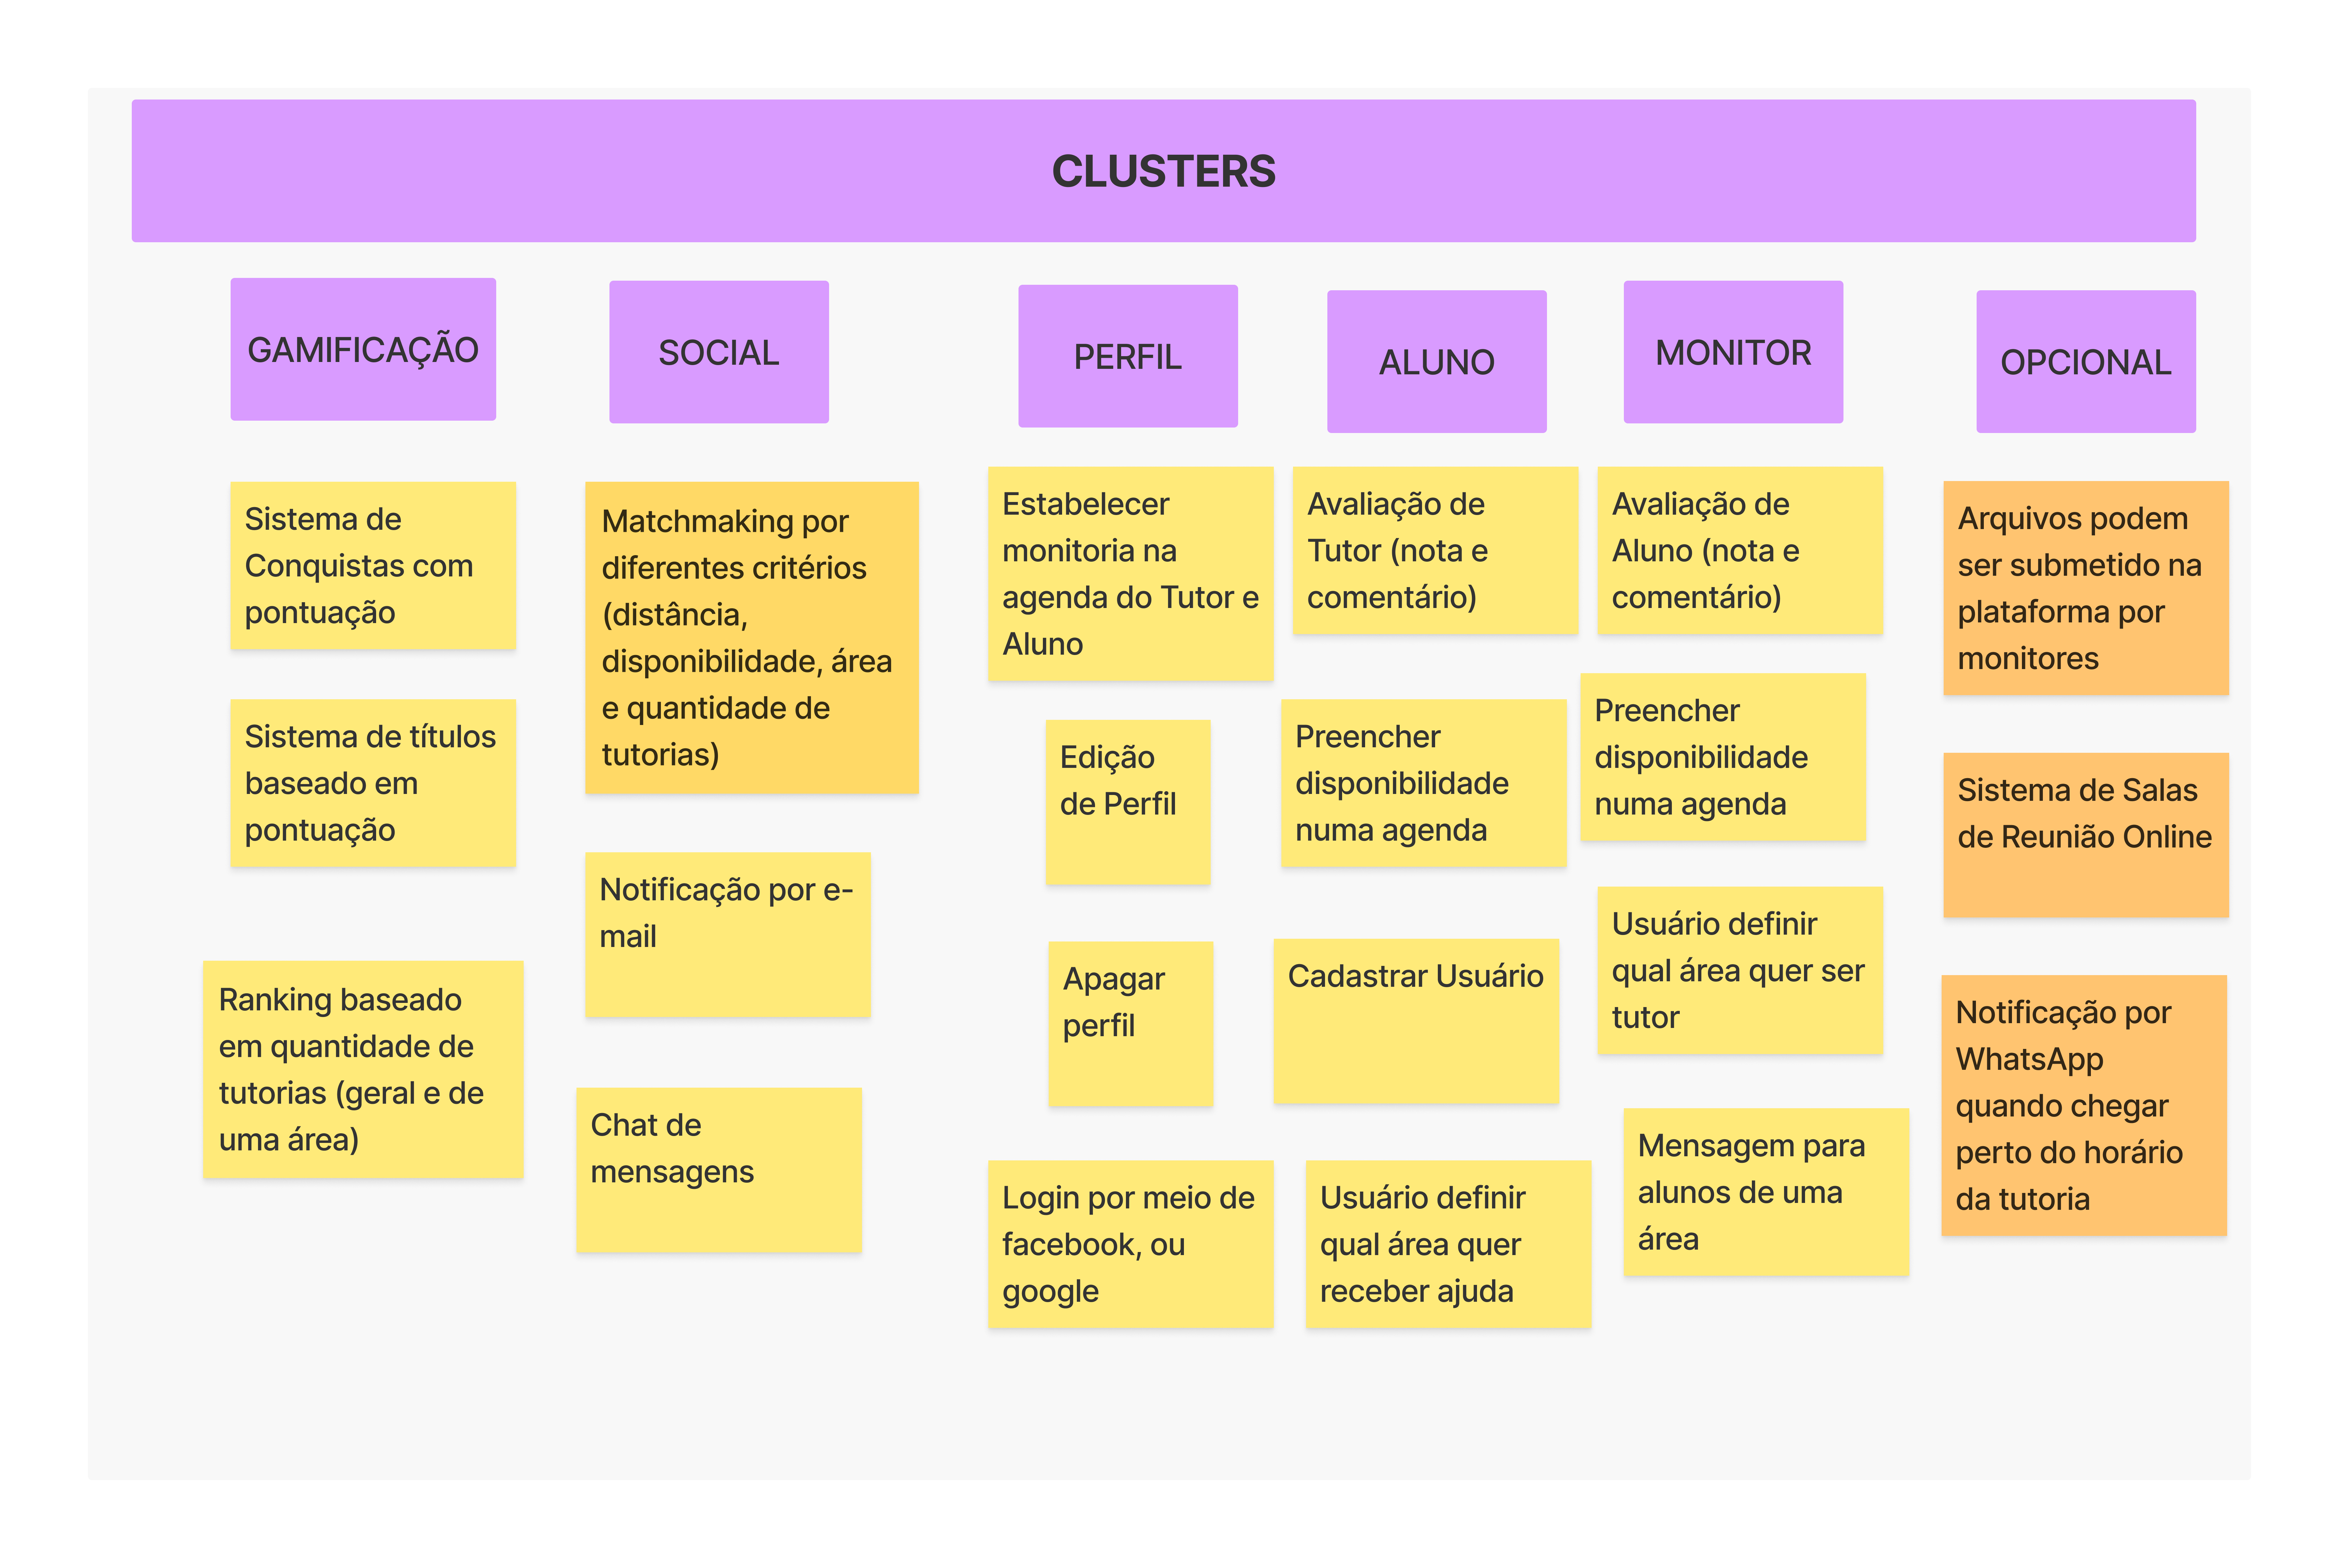
\includegraphics[width=1\textwidth]{figuras/Lean12Funcionalidades.png}

    Fonte: Adaptado a partir de caroli.org
    
    \vspace{0.2cm}
\end{figure}

\begin{figure}[h!]
    \centering
    \caption{Revisão técnica de negócio e de experiência de usuário (Gamificação, Social e Perfil).} 
    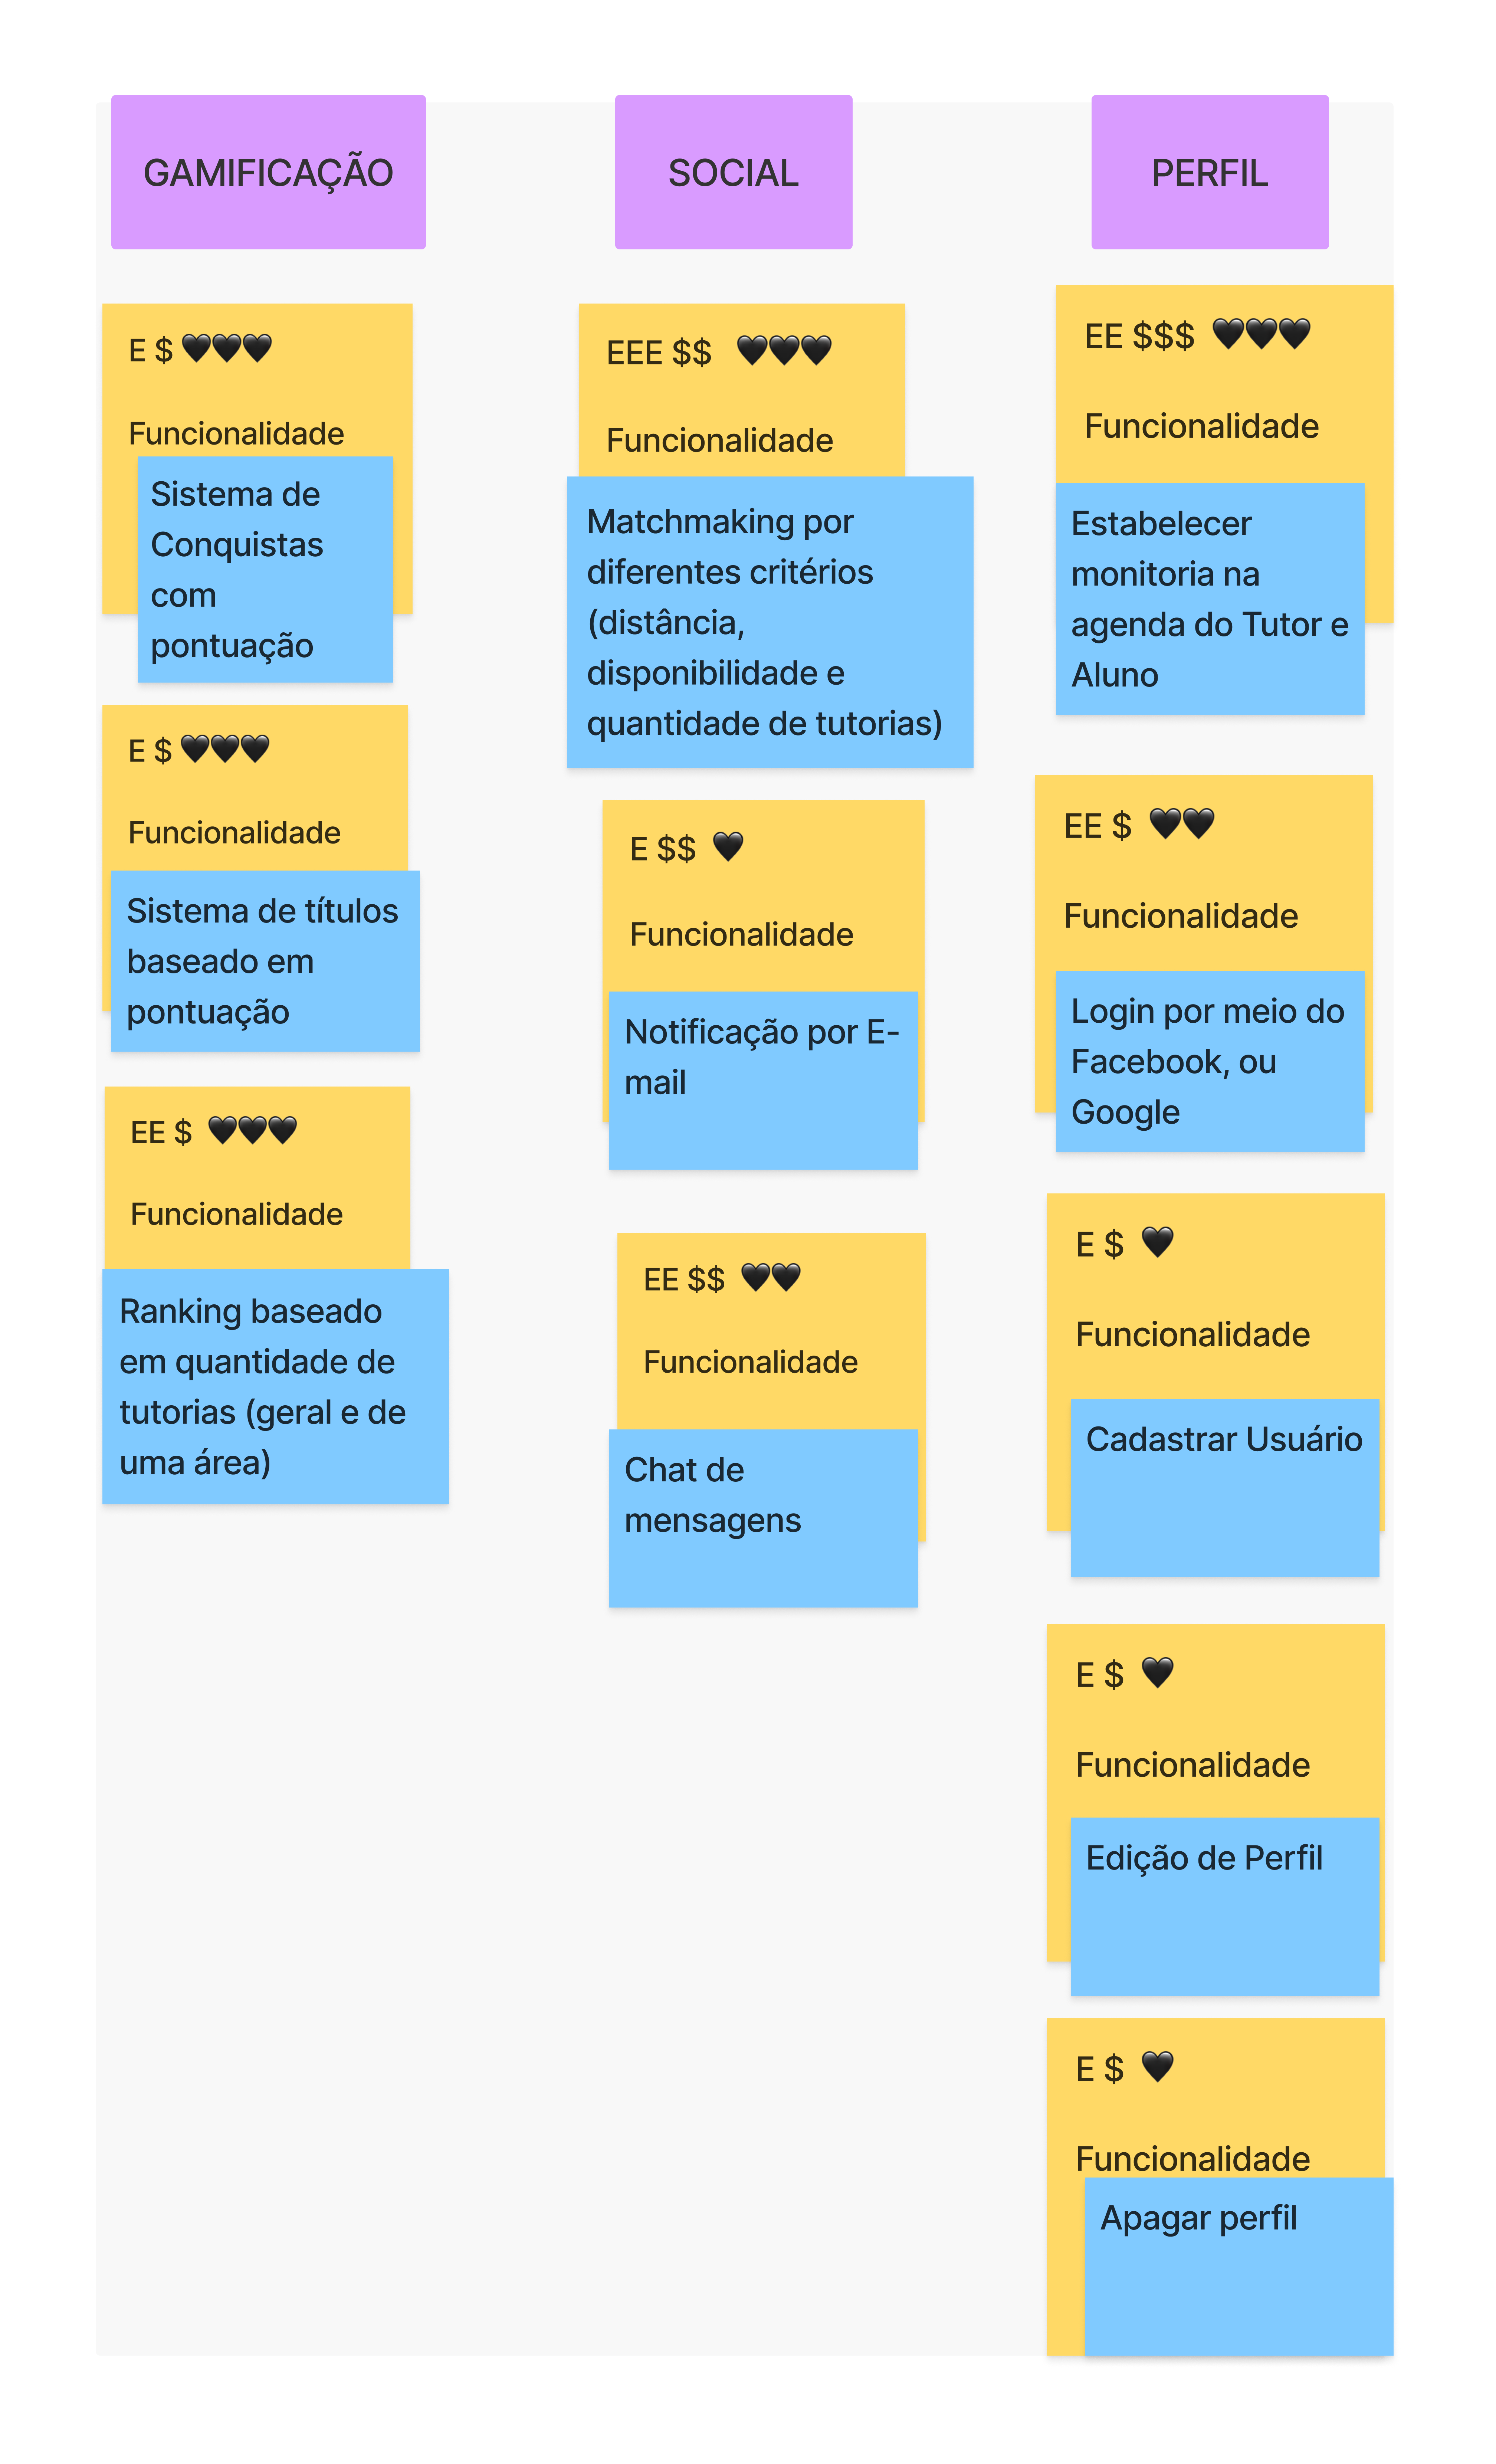
\includegraphics[width=0.7\textwidth]{figuras/Lean13Custos.png}

    Fonte: Adaptado a partir de caroli.org
    
    \vspace{0.2cm}
\end{figure}

\begin{figure}[h!]
    \centering
    \caption{Revisão técnica de negócio e de experiência de usuário (Aluno, Monitor e Opcional).} 
    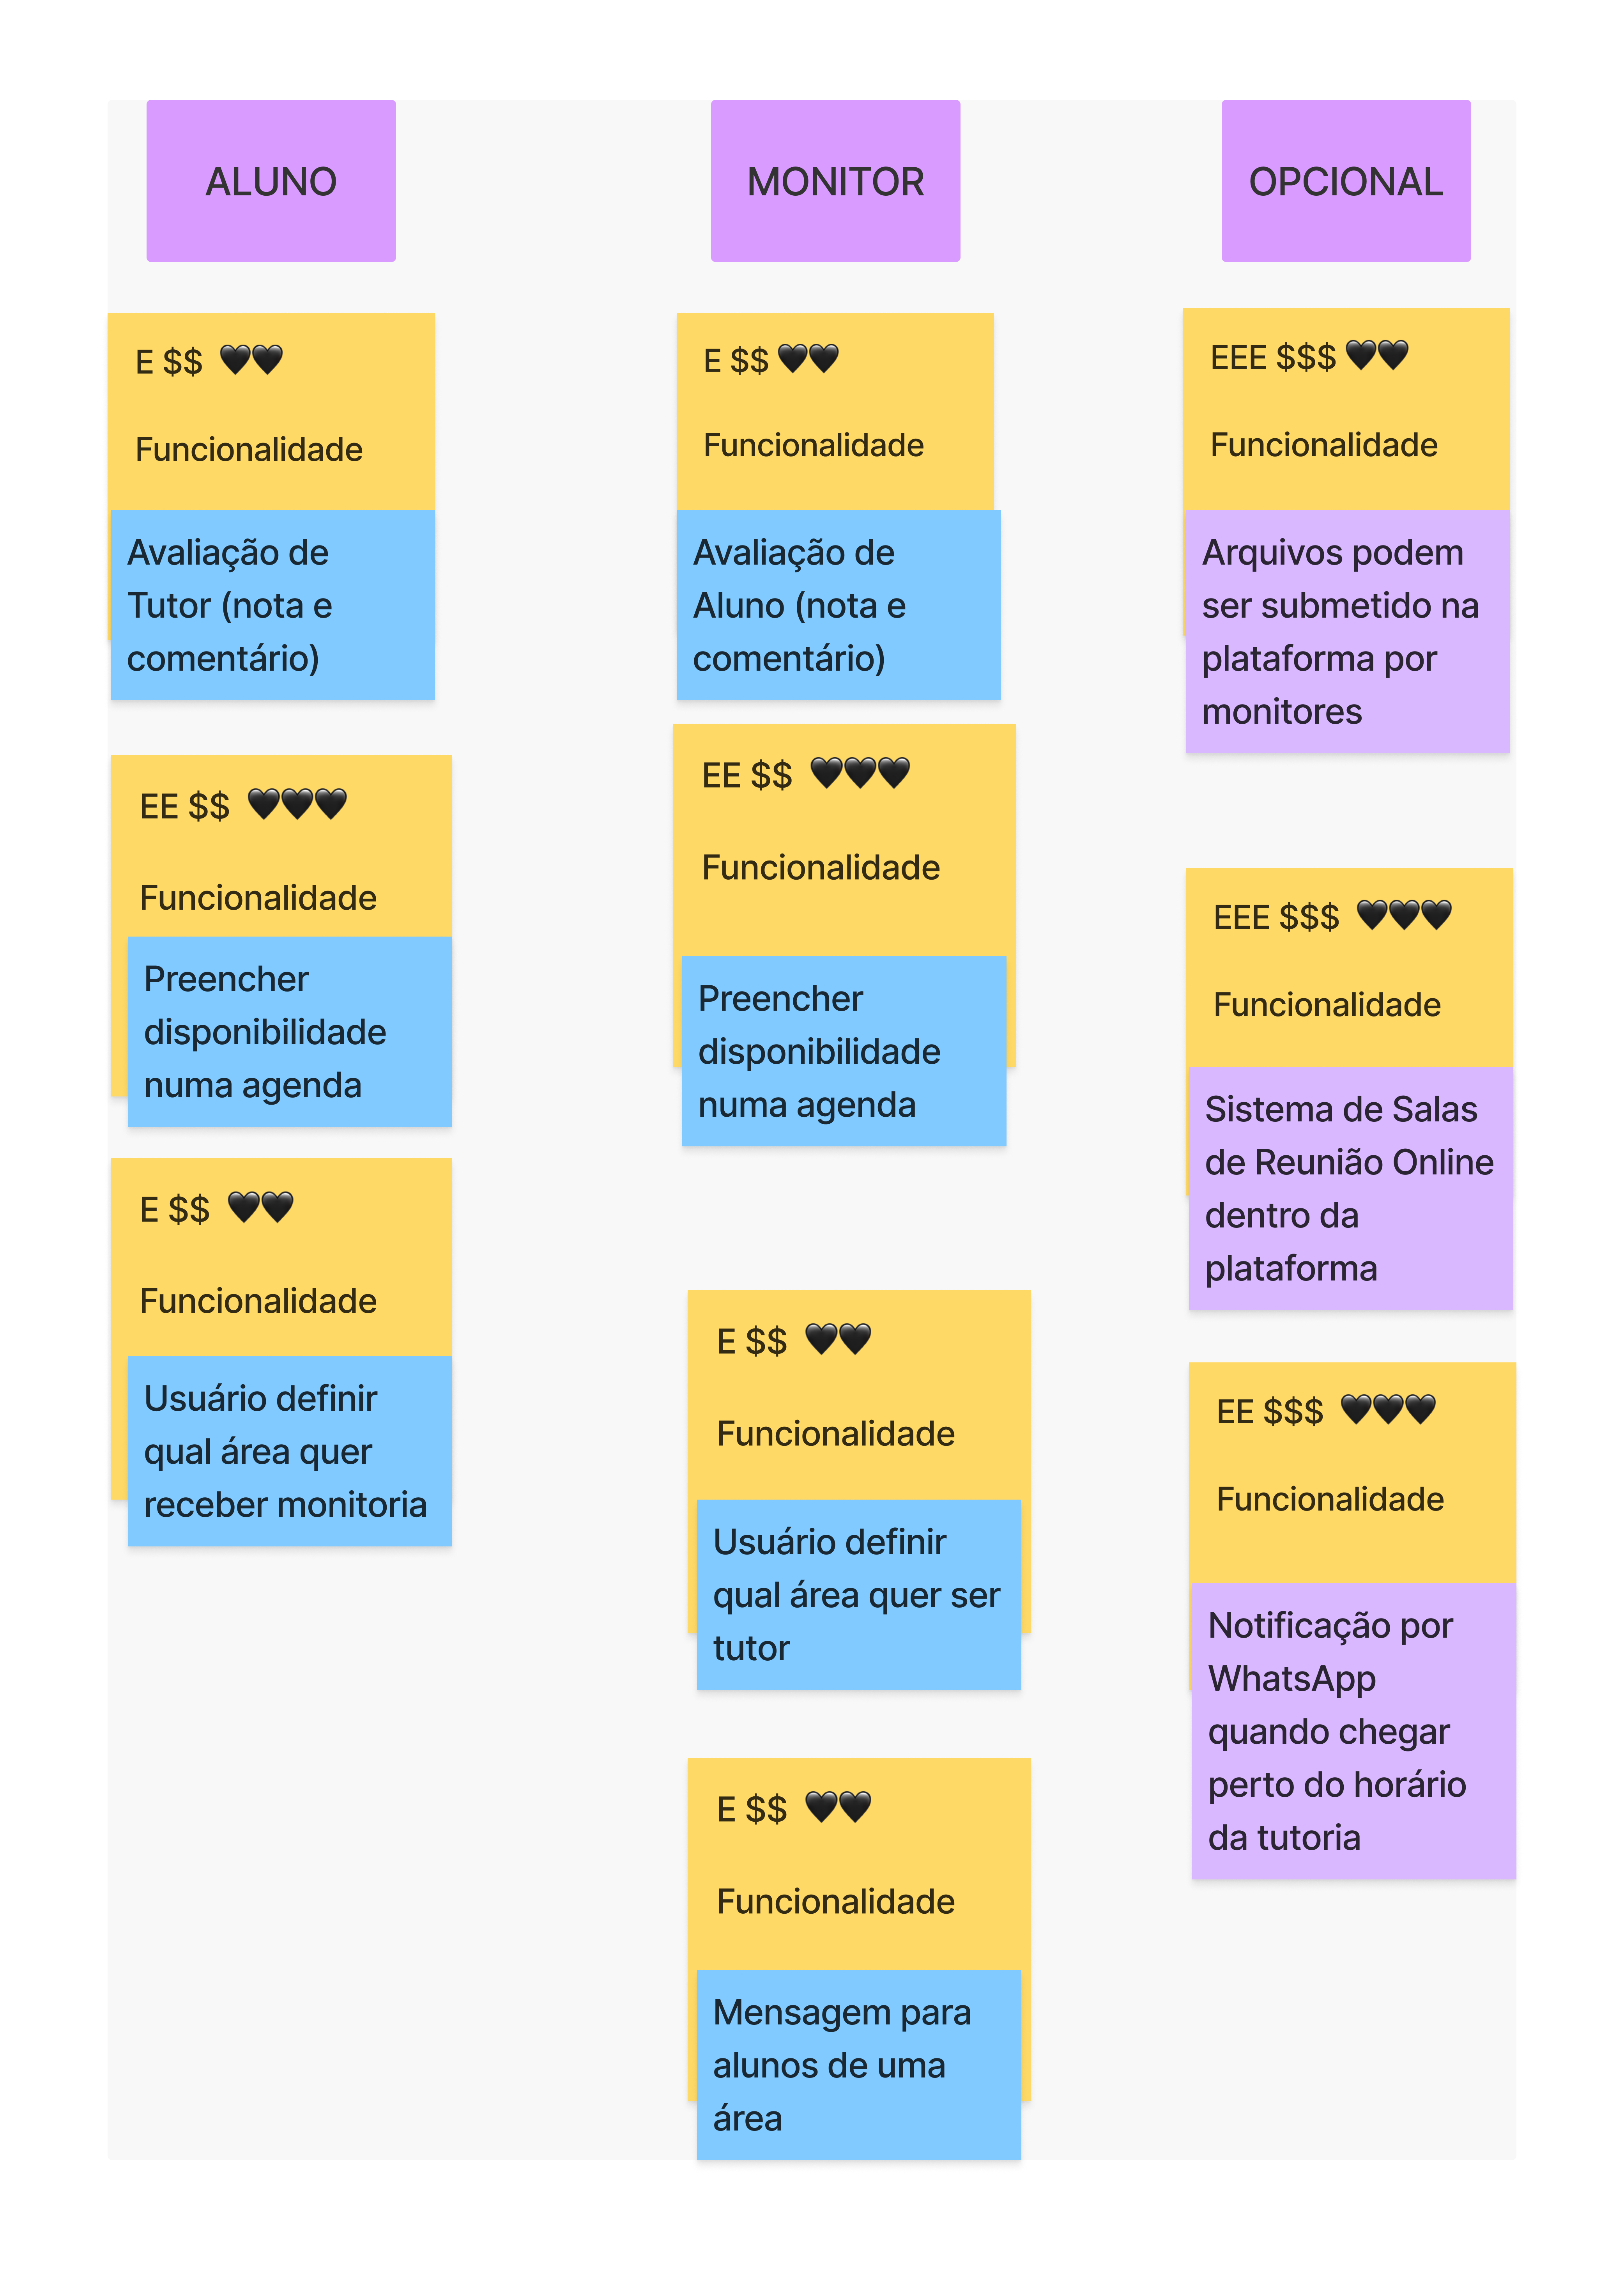
\includegraphics[width=0.7\textwidth]{figuras/Lean13Custos2.png}

    Fonte: Adaptado a partir de caroli.org
    
    \vspace{0.2cm}
\end{figure}

\begin{figure}[h!]
    \centering
    \caption{Sequenciador (quatro primeiros níveis).} 
    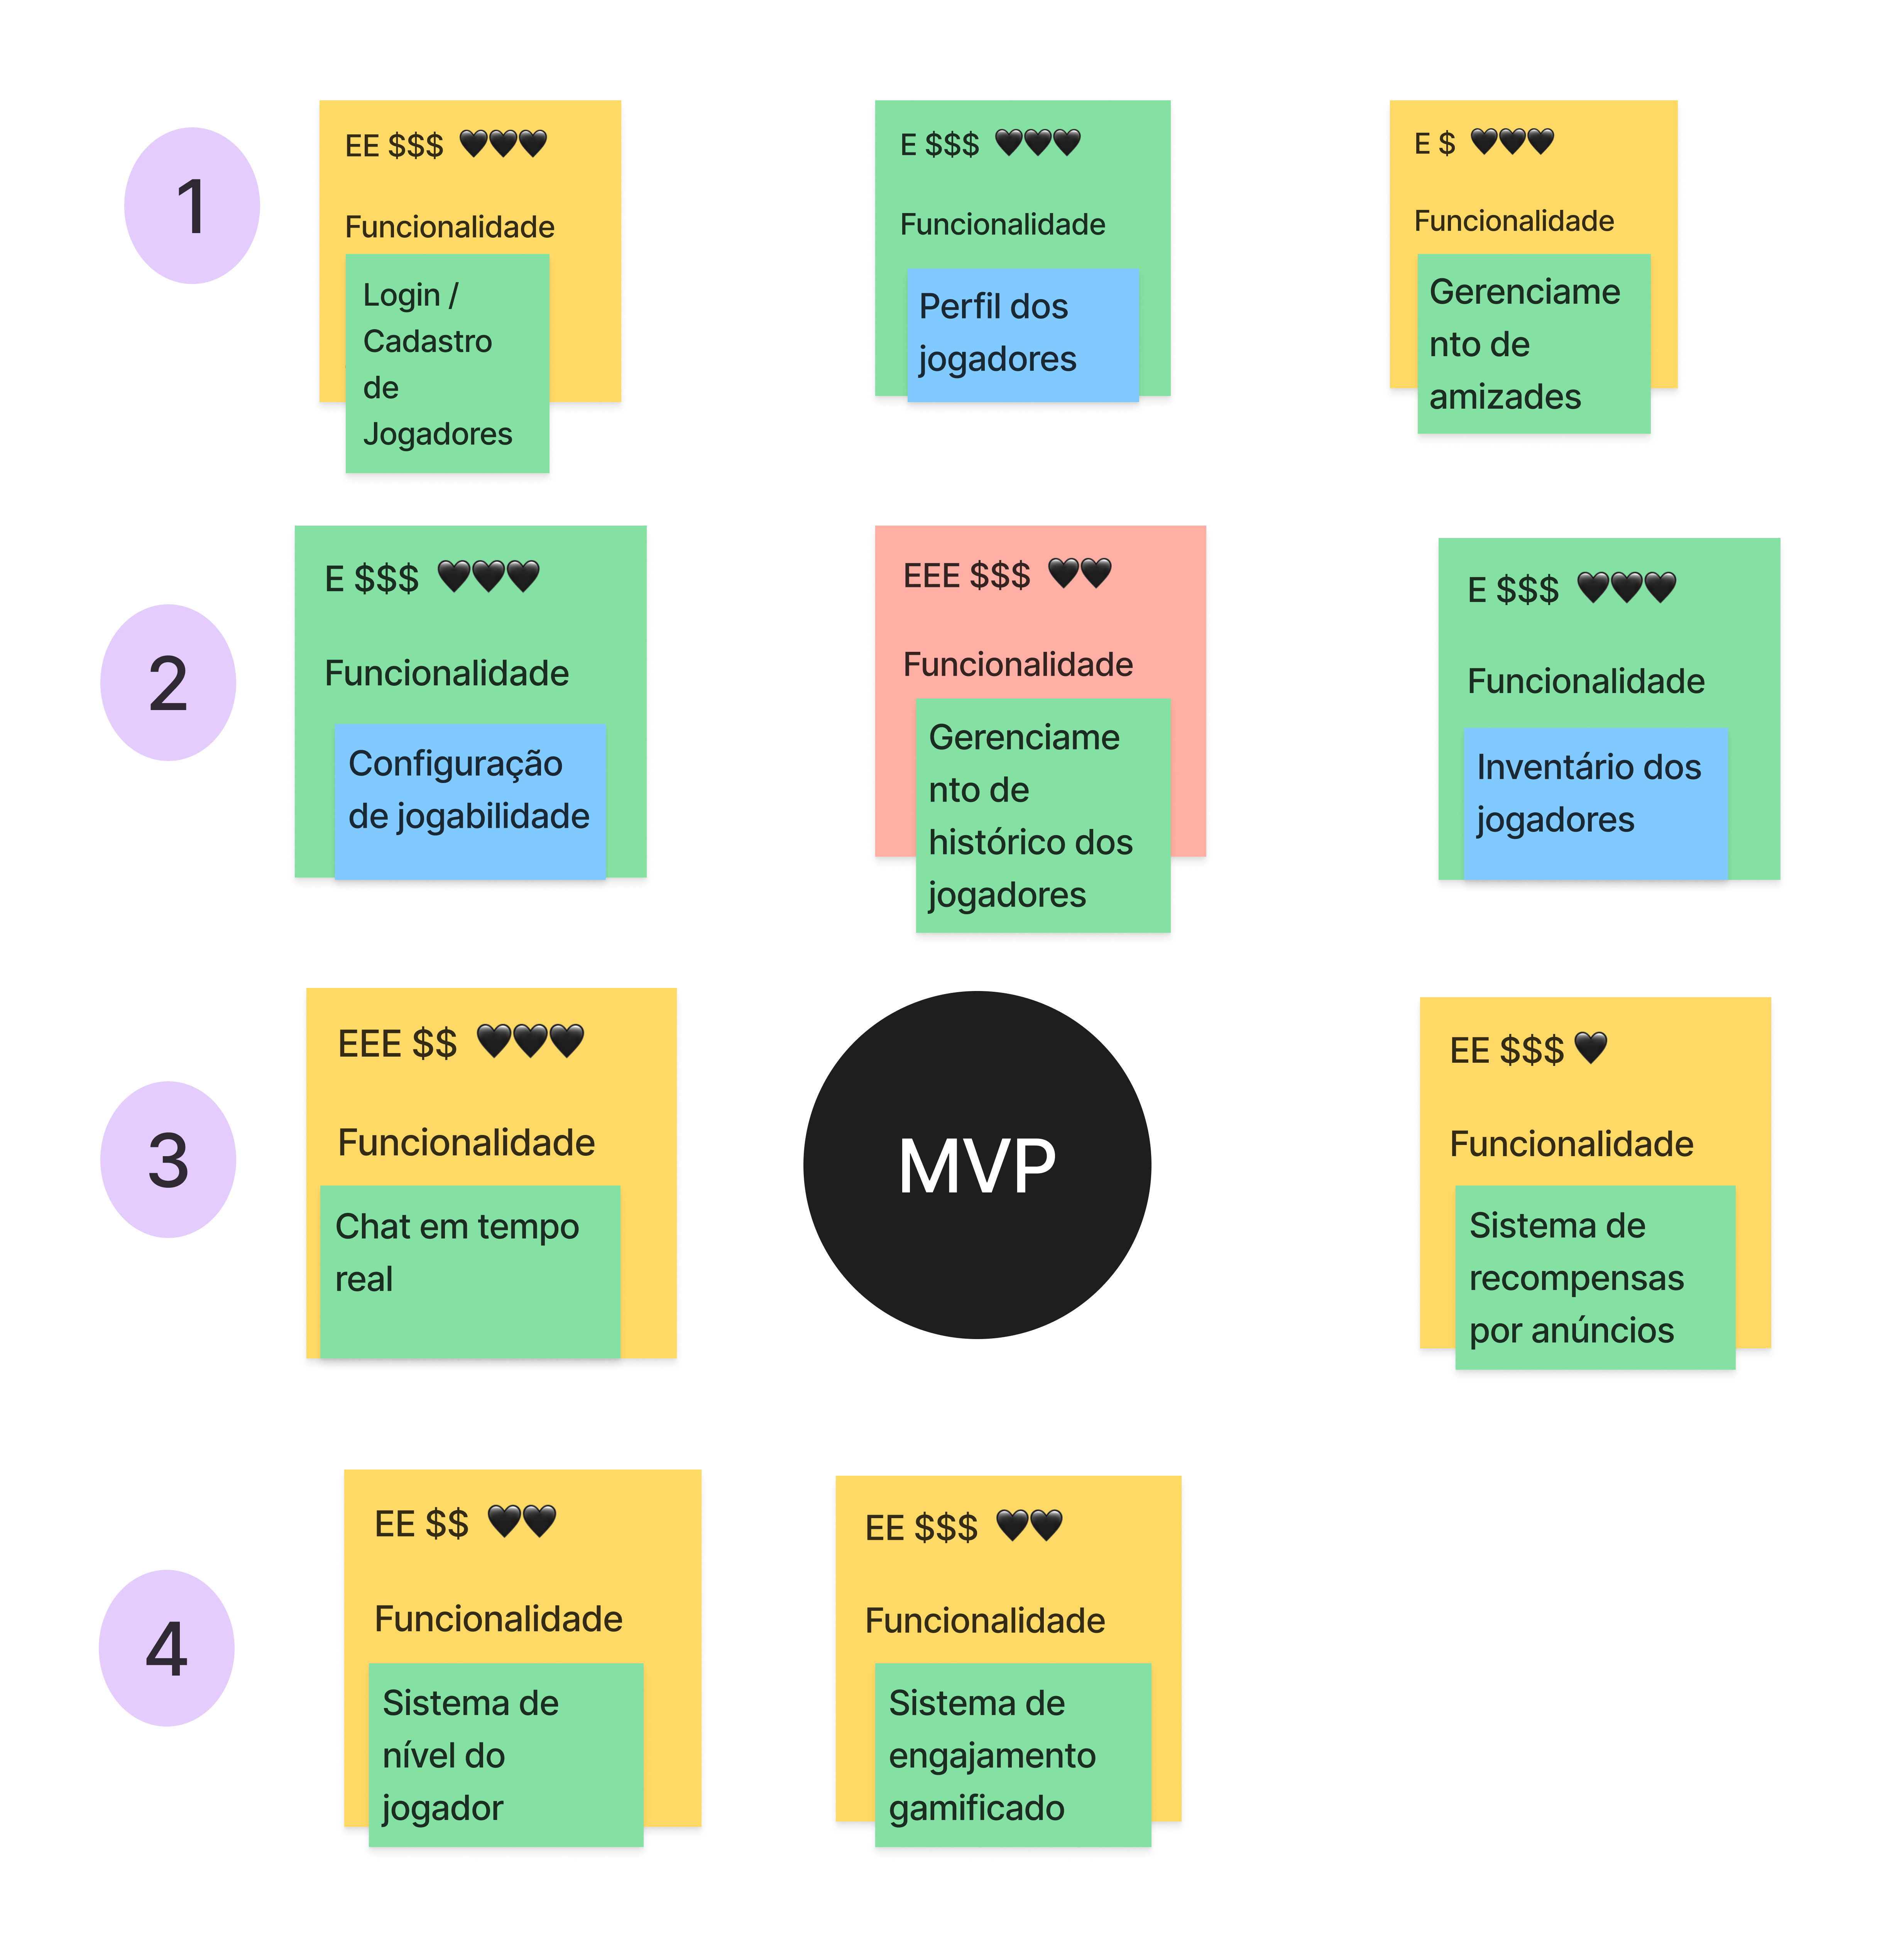
\includegraphics[width=0.9\textwidth]{figuras/Lean14Sequenciador.png}

    Fonte: Adaptado a partir de caroli.org
    
    \vspace{0.2cm}
\end{figure}

\begin{figure}[h!]
    \centering
    \caption{Sequenciador (últimos níveis).} 
    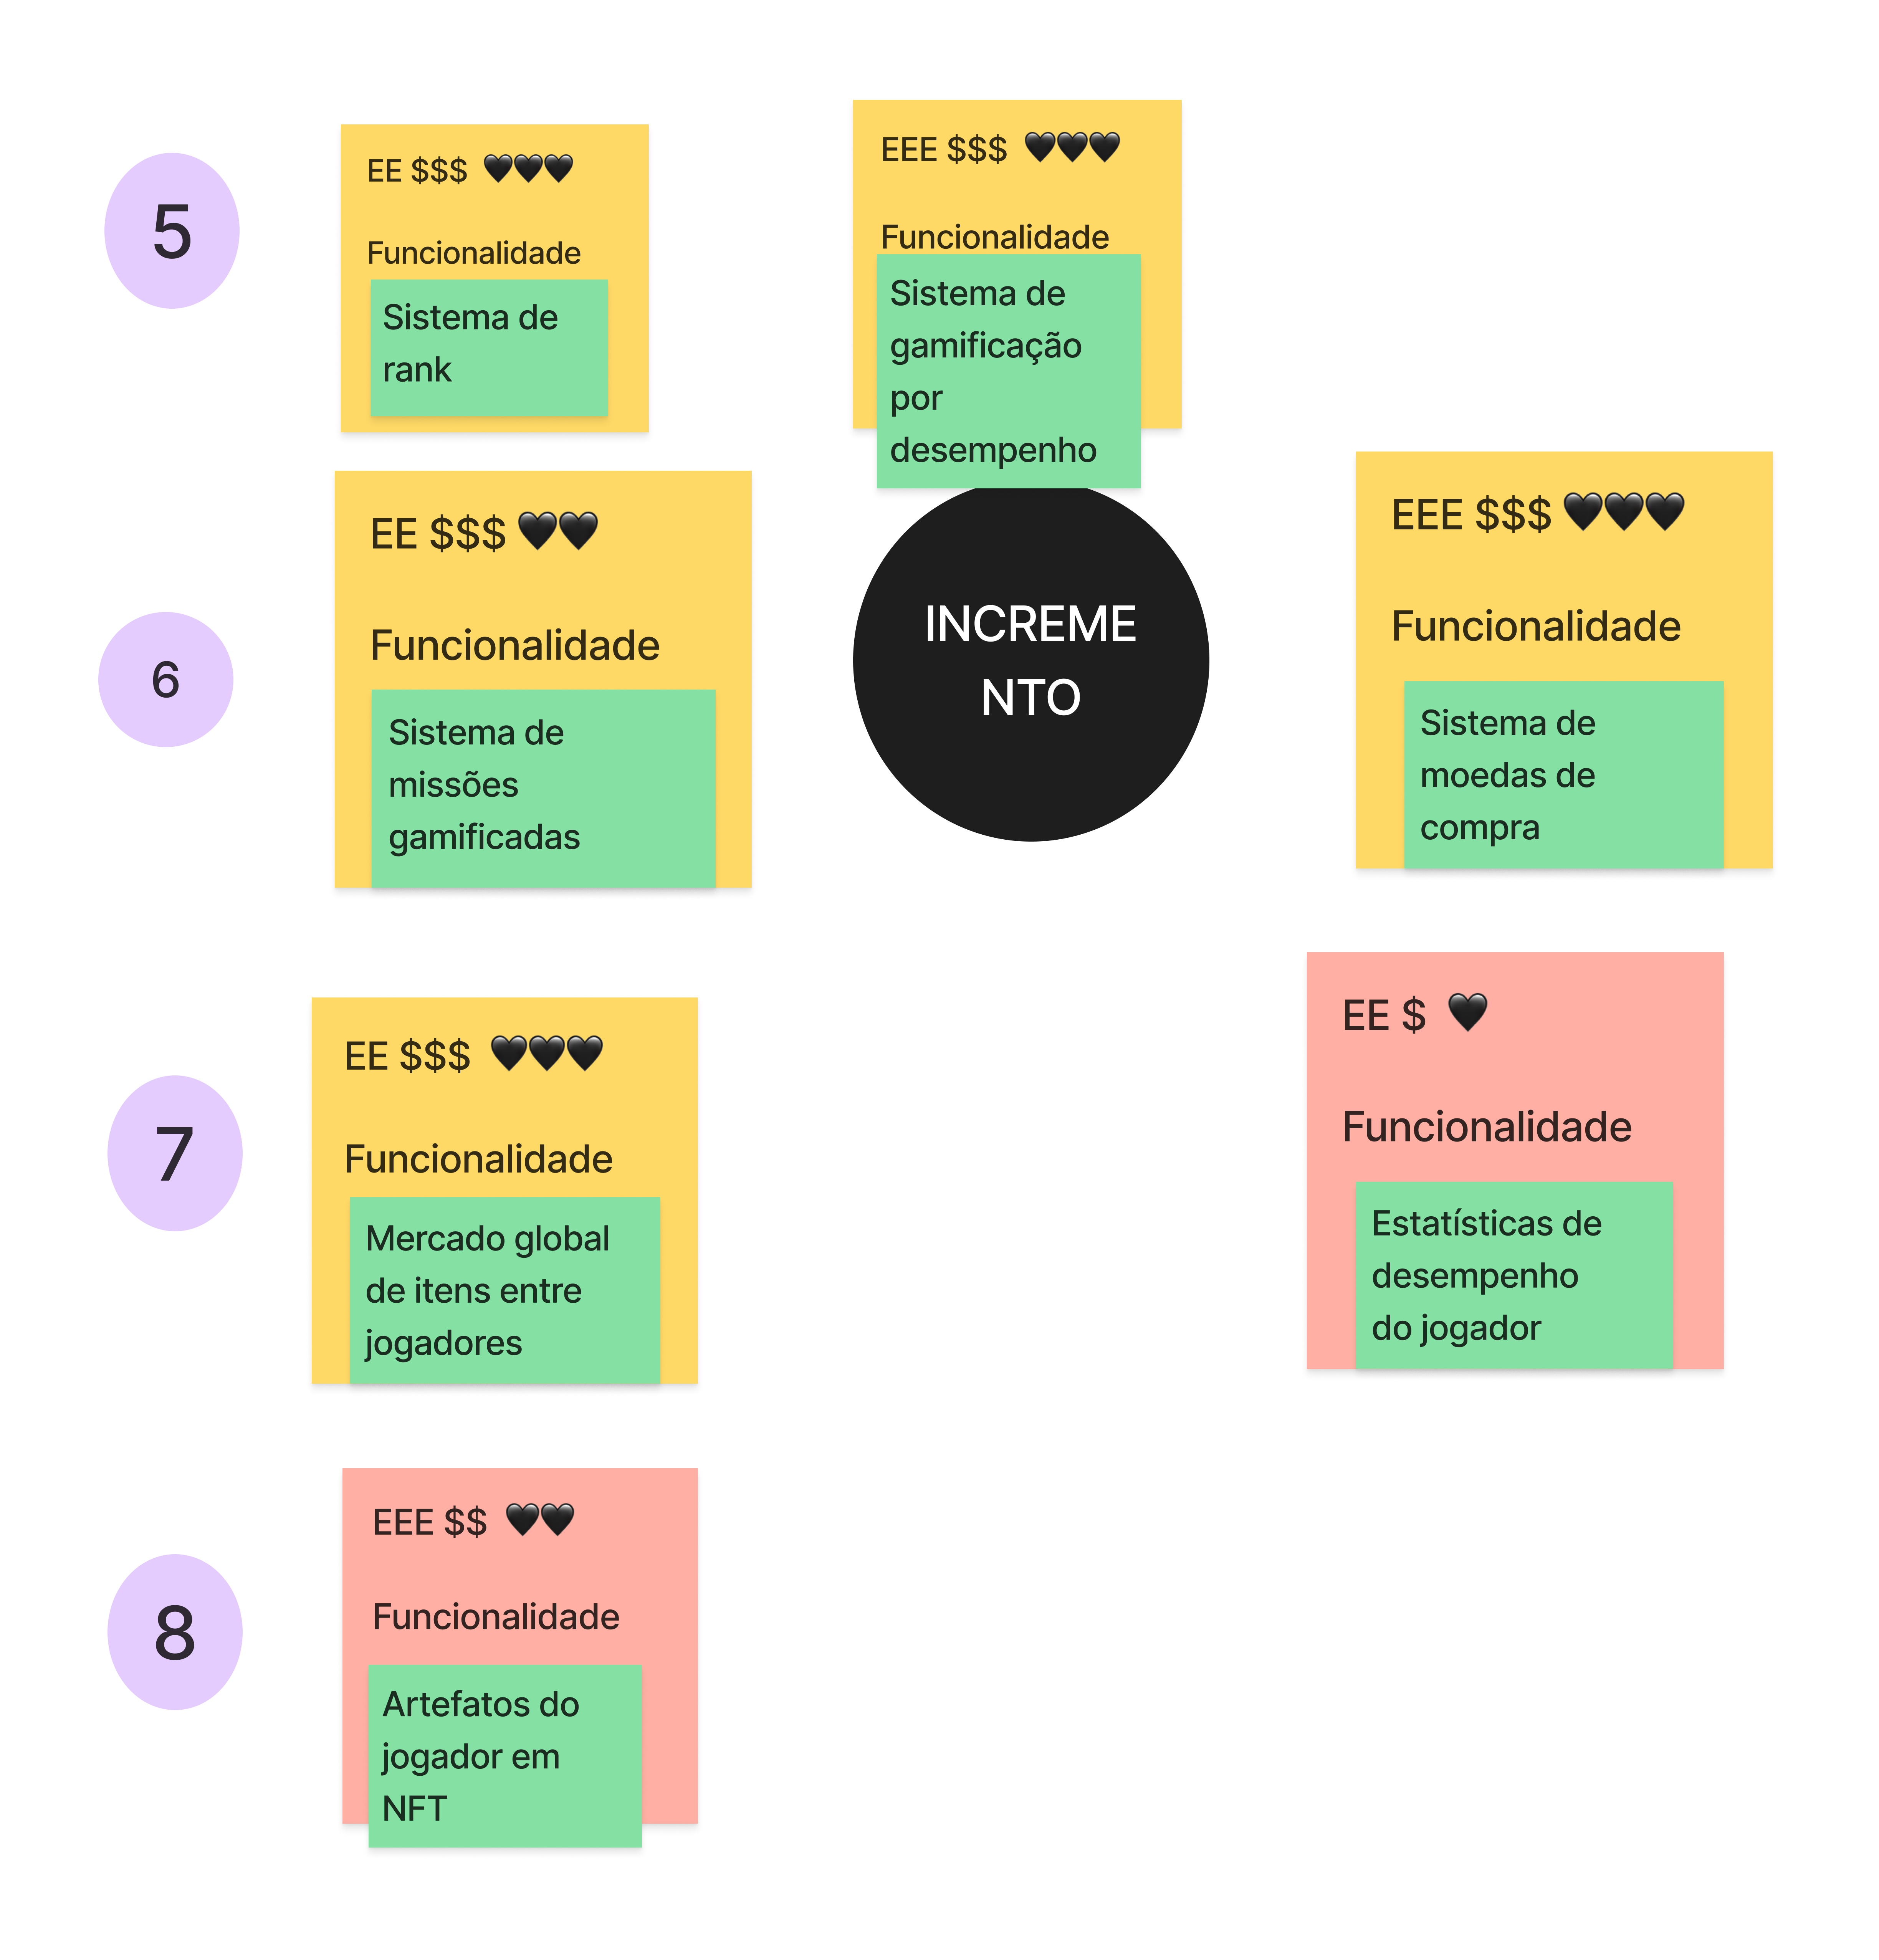
\includegraphics[width=0.9\textwidth]{figuras/Lean14Sequenciador2.png}

    Fonte: Adaptado a partir de caroli.org
    
    \vspace{0.2cm}
\end{figure}

\begin{figure}[h!]
    \centering
    \caption{Canvas MVP.} 
    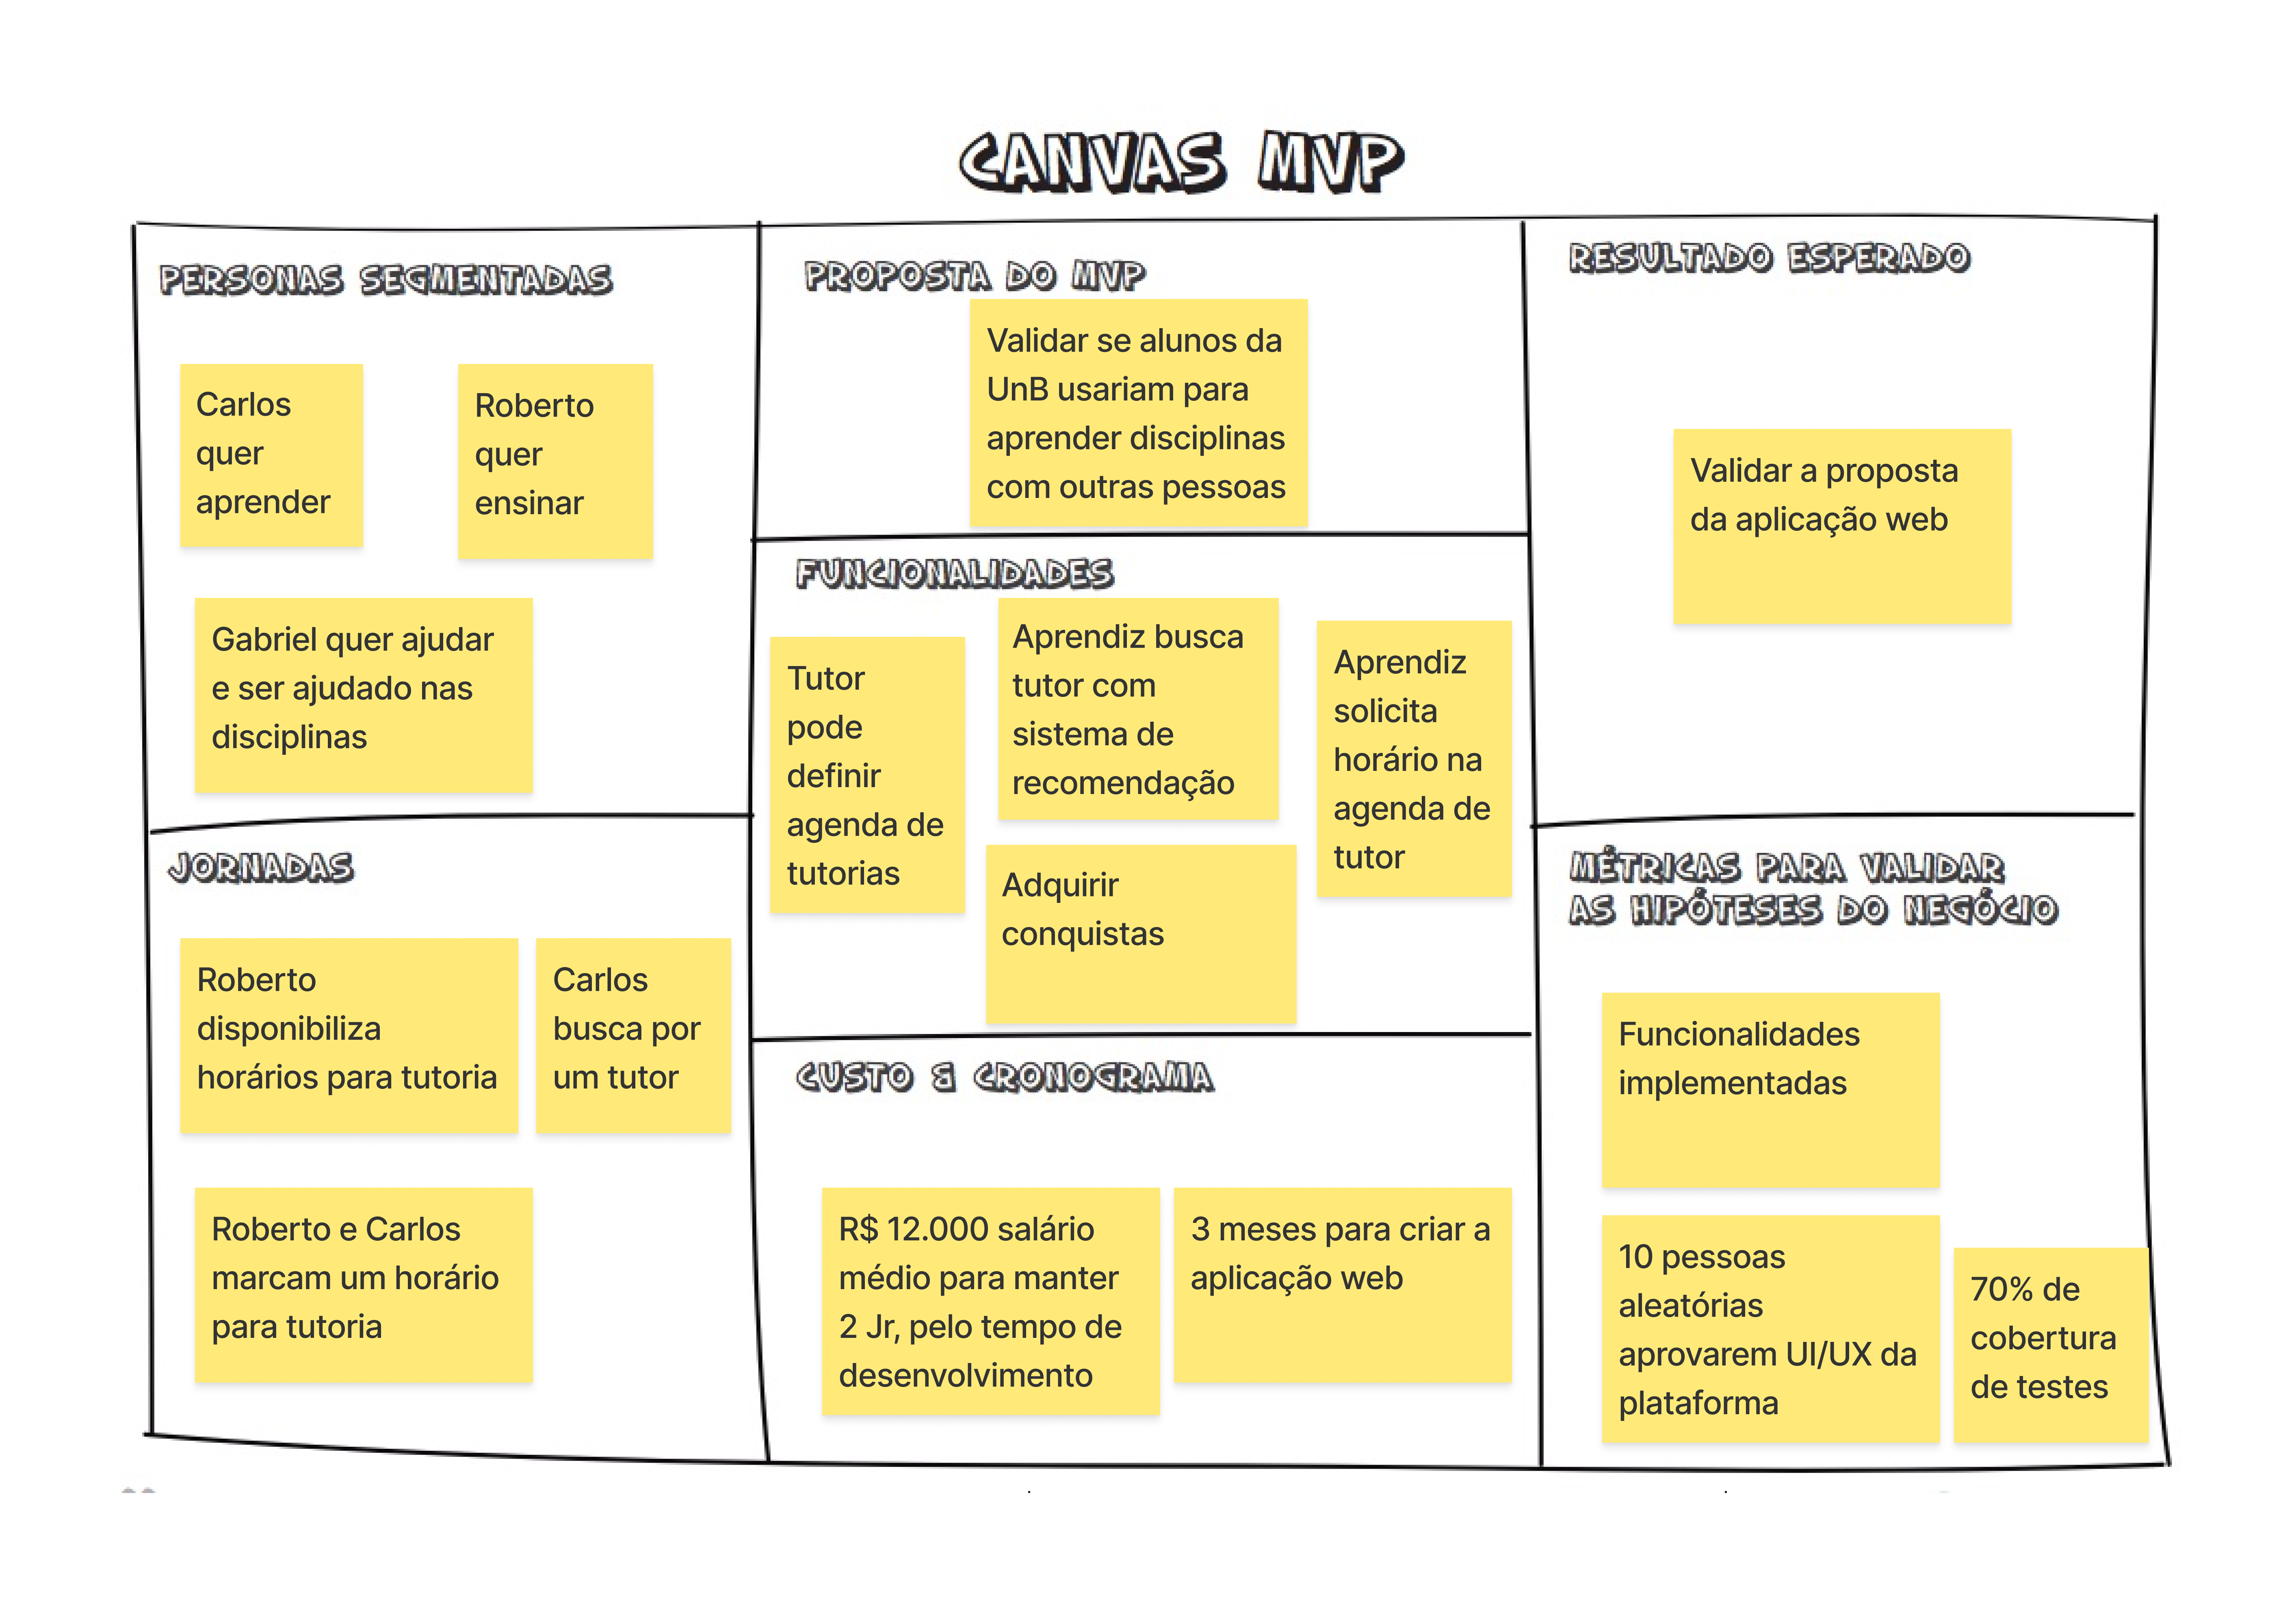
\includegraphics[width=1.1\textwidth]{figuras/Lean15Canvas.png}

    Fonte: Adaptado a partir de caroli.org
    
    \vspace{0.2cm}
\end{figure}

\chapter{Dicionário de Dados}
\label{dicionario-dados}

\section*{USUARIO}
\noindent\textbf{Esclarecimento Técnico:} Tabela proveniente de uma Entidade.\\
\textbf{Descrição:} Define os dados de um Usuário que será cadastrado. 

\begin{table}[h!]
    \centering
    \label{tab:usuario-apendice}
    \resizebox{\linewidth}{!}
    {% Redimensiona a tabela para caber na largura da página
    \begin{tabular}{|l|L{5.5cm}|l|l|L{4cm}|}
        \hline
        \textbf{Atributo} & \textbf{Propriedades do atributo} & \textbf{Tipo de dado} & \textbf{Tamanho} & \textbf{Descrição} \\
        \hline
        usuarioId & chave primária, obrigatório, autoincremento & int & & Número identificador do usuário \\
        \hline
        email & único, obrigatório & varchar & 254 & E-mail do usuário \\
        \hline
        senha & obrigatório & varchar & 256 & Senha criptografada do usuário \\
        \hline
        nomePerfil & obrigatório & varchar & 100 & Nome exibido no perfil do usuário \\
        \hline
        cidade & optativo & varchar & 80 & Cidade onde reside o usuário \\
        \hline
        estado & optativo & char & 2 & Estado onde reside o usuário \\
        \hline
        pontuacao & obrigatório & unsigned int & & Quantidade de pontos obtidos por conquistas do usuário \\
        \hline
        urlFoto & obrigatório & varchar & 256 & URL da foto exibida no perfil do usuário \\
        \hline
        mediaNotaAprendiz & \begin{tabular}[c]{@{}l@{}}derivado de valores na tabela \\ AVALIACAO\_APRENDIZ e \\ não é armazenado por 3ª \\ Forma Normal\end{tabular} & - & - & Média das avaliações do usuário como aprendiz \\
        \hline
    \end{tabular}%
    }
\end{table}

\section*{TUTOR}
\noindent\textbf{Esclarecimento Técnico:} Tabela proveniente de uma Entidade. \\
\textbf{Descrição:} Define os dados de um Tutor que será cadastrado. 

\begin{table}[h!]
\centering
\label{tab:tutor}
\resizebox{\linewidth}{!}{% Redimensiona a tabela para caber na largura da página
    \begin{tabular}{|l|L{3cm}|l|l|l|}
        \hline
        \textbf{Atributo} & \textbf{Propriedades do atributo} & \textbf{Tipo de dado} & \textbf{Tamanho} & \textbf{Descrição} \\
        \hline
        tutorId & chave primária, obrigatório, autoincremento & int & & Número identificador do tutor \\
        \hline
        usuarioId & chave estrangeira, obrigatório & int & & Número identificador do usuário \\
        \hline
    \end{tabular}
}
\end{table}

\section*{AVALIACAO\_APRENDIZ}
\noindent\textbf{Esclarecimento Técnico:} Tabela proveniente de uma Entidade. \\
\textbf{Descrição:} Define os dados de uma avaliação de um aprendiz que será cadastrada.

\begin{table}[h!]
\centering
\label{tab:avaliacao_aprendiz}
    \resizebox{\linewidth}{!}{% Redimensiona a tabela para caber na largura da página
    \begin{tabular}{|l|l|l|l|L{4.5cm}|}
        \hline
        \textbf{Atributo} & \textbf{Propriedades do atributo} & \textbf{Tipo de dado} & \textbf{Tamanho} & \textbf{Descrição} \\
        \hline
        usuarioId & chave estrangeira, obrigatório & int & & Número identificador do usuário \\
        \hline
        nota & obrigatório & int & 1 & Nota fornecida para a avaliação do aprendiz, de 1 a 5. \\
        \hline
        comentario & optativo & varchar & 200 & Comentário fornecido para a avaliação do aprendiz \\
        \hline
    \end{tabular}
    }
\end{table}

\section*{AVALIACAO\_TUTOR}
\noindent\textbf{Esclarecimento Técnico:} Tabela proveniente de uma Entidade. \\
\textbf{Descrição:} Define os dados de uma avaliação de um tutor que será cadastrada.

\begin{table}[h!]
\centering
\label{tab:avaliacao_tutor}
\resizebox{\linewidth}{!}{% Redimensiona a tabela para caber na largura da página
    \begin{tabular}{|l|l|l|l|L{4.5cm}|}
        \hline
        \textbf{Atributo} & \textbf{Propriedades do atributo} & \textbf{Tipo de dado} & \textbf{Tamanho} & \textbf{Descrição} \\
        \hline
        tutorId & chave estrangeira, obrigatório & int & & Número identificador do tutor \\
        \hline
        nota & obrigatório & int & 1 & Nota fornecida para a avaliação do aprendiz, de 1 a 5. \\
        \hline
        comentario & optativo & varchar & 200 & Comentário fornecido para a avaliação do aprendiz \\
        \hline
    \end{tabular}
    }
\end{table}

\section*{AREA}
\noindent\textbf{Esclarecimento Técnico:} Tabela proveniente de uma Entidade.\\
\textbf{Descrição:} Define os dados de uma área de conhecimento que será cadastrada. 
\begin{table}[h!]
\centering
\label{tab:area}
\resizebox{\linewidth}{!}{% Redimensiona a tabela para caber na largura da página
    \begin{tabular}{|l|L{3cm}|l|l|l|}
        \hline
        \textbf{Atributo} & \textbf{Propriedades do atributo} & \textbf{Tipo de dado} & \textbf{Tamanho} & \textbf{Descrição} \\
        \hline
        areaId & chave primária, obrigatório, autoincremento & int & & Número identificador da área \\
        \hline
        nomeArea & único, obrigatório & varchar & 60 & Nome da área de conhecimento \\
        \hline
    \end{tabular}
    }
\end{table}

\section*{ESPECIALIDADE}
\noindent\textbf{Esclarecimento Técnico:} Tabela proveniente de uma Entidade. \\
\textbf{Descrição:} Define os dados de uma especialidade de uma área de conhecimento que será cadastrada. 

\begin{table}[h!]
\centering
\label{tab:especialidade}
\resizebox{\linewidth}{!}{% Redimensiona a tabela para caber na largura da página
\begin{tabular}{|l|L{3.5cm}|l|l|L{4cm}|}
\hline
\textbf{Atributo} & \textbf{Propriedades do atributo} & \textbf{Tipo de dado} & \textbf{Tamanho} & \textbf{Descrição} \\
\hline
especialidadeId & chave primária, obrigatório, autoincremento & int & & Número identificador da especialidade \\
\hline
areaId & chave estrangeira, chave única composta, obrigatório & int & & Número identificador da área de conhecimento \\
\hline
nomeEspecialidade & chave única composta, obrigatório & varchar & 100 & Nome da especialidade \\
\hline
\end{tabular}
}
\end{table}

\section*{CONQUISTA}
\noindent\textbf{Esclarecimento Técnico:} Tabela proveniente de uma Entidade. \\
\textbf{Descrição:} Define os dados de uma conquista que será cadastrada.

\begin{table}[h!]
\centering
\label{tab:conquista}
\resizebox{\linewidth}{!}{% Redimensiona a tabela para caber na largura da página
\begin{tabular}{|l|L{3.5cm}|l|l|L{5cm}|}
\hline
\textbf{Atributo} & \textbf{Propriedades do atributo} & \textbf{Tipo de dado} & \textbf{Tamanho} & \textbf{Descrição} \\
\hline
conquistaId & chave primária, obrigatório, autoincremento & int & & Número identificador da conquista \\
\hline
titulo & único, obrigatório & varchar & 32 & Título da conquista \\
\hline
descricao & obrigatório & varchar & 64 & Descrição do que deve ser feito para conseguir a conquista \\
\hline
urlImagem & obrigatório & varchar & 256 & URL da imagem da conquista \\
\hline
pontos & obrigatório & int & & Quantidade de pontos que serão recompensados ao usuário que conseguir a conquista \\
\hline
\end{tabular}%
}
\end{table}

\section*{CHAT}
\noindent\textbf{Esclarecimento Técnico:} Tabela proveniente de uma Entidade. \\
\textbf{Descrição:} Define os dados de um chat de mensagens entre um tutor e um aprendiz que será cadastrado.

\newpage

\begin{table}[h!]
\centering
\label{tab:chat}
\resizebox{\linewidth}{!}{% Redimensiona a tabela para caber na largura da página
\begin{tabular}{|l|L{3cm}|l|l|l|}
\hline
\textbf{Atributo} & \textbf{Propriedades do atributo} & \textbf{Tipo de dado} & \textbf{Tamanho} & \textbf{Descrição} \\
\hline
chatId & chave primária, obrigatório, autoincremento & int & & Número identificador do chat \\
\hline
tutorId & chave estrangeira, chave única composta, obrigatório & int & & Número identificador do tutor \\
\hline
usuarioId & chave estrangeira, chave única composta, obrigatório & int & & Número identificador do aprendiz \\
\hline
\end{tabular}
}
\end{table}

\section*{MENSAGEM}
\noindent\textbf{Esclarecimento Técnico:} Tabela proveniente de uma Entidade. \\
\textbf{Descrição:} Define os dados de uma mensagem enviada para um chat de mensagens entre um tutor e um aprendiz que será cadastrada.

\begin{table}[h!]
\centering
\label{tab:mensagem}
\resizebox{\linewidth}{!}{% Redimensiona a tabela para caber na largura da página
\begin{tabular}{|l|l|L{3.5cm}|l|L{4cm}|}
\hline
\textbf{Atributo} & \textbf{Propriedades do atributo} & \textbf{Tipo de dado} & \textbf{Tamanho} & \textbf{Descrição} \\
\hline
chatId & chave estrangeira, obrigatório & int & & Número identificador do chat \\
\hline
conteudo & obrigatório & varchar & 200 & Conteúdo textual da mensagem \\
\hline
horario & obrigatório & datetime & & Data e horário de envio da mensagem \\
\hline
remetente & obrigatório & enum('TUTOR', 'APRENDIZ') & & Identificador de quem mandou a mensagem no chat \\
\hline
\end{tabular}
}
\end{table}

\section*{SESSAO}
\noindent\textbf{Esclarecimento Técnico:} Tabela proveniente de uma Entidade. \\
\textbf{Descrição:} Define os dados de uma sessão de tutoria disponível na agenda de um tutor que serão cadastrados.

\newpage

\begin{table}[h!]
\centering
\label{tab:sessao}
\resizebox{\linewidth}{!}{% Redimensiona a tabela para caber na largura da página
\begin{tabular}{|l|L{3cm}|L{3.5cm}|l|L{3.5cm}|}
\hline
\textbf{Atributo} & \textbf{Propriedades do atributo} & \textbf{Tipo de dado} & \textbf{Tamanho} & \textbf{Descrição} \\
\hline
sessaoId & chave primária, obrigatório, autoincremento & int & & Número identificador da sessão \\
\hline
tutorId & chave estrangeira, chave única composta, obrigatório & int & & Número identificador do tutor \\
\hline
dia & chave única composta, obrigatório & enum('SEG', 'TER', 'QUA', 'QUI', 'SEX', 'SAB', 'DOM') & & Dia disponível na agenda do tutor \\
\hline
horarioInicio & chave única composta, obrigatório & time & & Horário de início de uma sessão de tutoria disponível do tutor \\
\hline
horarioFim & obrigatório & time & & Horário de fim de uma sessão de tutoria disponível do tutor \\
\hline
\end{tabular}
}
\end{table}

\section*{SOLICITAÇÃO}
\noindent\textbf{Esclarecimento Técnico:} Tabela proveniente de uma Entidade. \\
\textbf{Descrição:} Define os dados de uma solicitação de sessão de tutoria realizada por um aprendiz que será cadastrada.

\begin{table}[h!]
\centering
\label{tab:solicitacao}
\resizebox{\linewidth}{!}{% Redimensiona a tabela para caber na largura da página
\begin{tabular}{|l|l|L{3cm}|l|L{3cm}|}
\hline
\textbf{Atributo} & \textbf{Propriedades do atributo} & \textbf{Tipo de dado} & \textbf{Tamanho} & \textbf{Descrição} \\
\hline
usuarioId & chave estrangeira, obrigatório & int & & Número identificador do aprendiz \\
\hline
sessaoId & chave estrangeira, obrigatório & int & & Número identificador da sessão \\
\hline
dataCriacao & obrigatório & datetime & & Data e horário da solicitação \\
\hline
validade & obrigatório & datetime & & Data e horário de validade da solicitação \\
\hline
estado & obrigatório & enum('ACEITO', 'PENDENTE', 'RECUSADO', 'RECORRENTE') & & Estado da solicitação \\
\hline
\end{tabular}
}
\end{table}

\section*{CONTEM}
\noindent\textbf{Esclarecimento Técnico:} Tabela proveniente de um Relacionamento.  \\
\textbf{Descrição:} Define relacionamento que corresponde a um relacionamento entre TUTOR e ESPECIALIDADE com cardinalidade \textbf{n:m}.

\begin{table}[h!]
\centering
\label{tab:contem}
\resizebox{\linewidth}{!}{% Redimensiona a tabela para caber na largura da página
\begin{tabular}{|l|L{3.5cm}|l|l|L{3cm}|}
\hline
\textbf{Atributo} & \textbf{Propriedades do atributo} & \textbf{Tipo de dado} & \textbf{Tamanho} & \textbf{Descrição} \\
\hline
especialidadeId & chave estrangeira, chave única composta, obrigatório & int & & Número identificador da especialidade \\
\hline
tutorId & chave estrangeira, chave única composta, obrigatório & int & & Número identificador do tutor \\
\hline
\end{tabular}
}
\end{table}

\section*{CONSEGUE}
\noindent\textbf{Esclarecimento Técnico:} Tabela proveniente de um Relacionamento. \\
\textbf{Descrição:} Define relacionamento que corresponde a um relacionamento entre USUARIO e CONQUISTA com cardinalidade \textbf{n:m}.

\begin{table}[h!]
\centering
\label{tab:consegue}
\resizebox{\linewidth}{!}{% Redimensiona a tabela para caber na largura da página
\begin{tabular}{|l|L{3.5cm}|l|l|l|}
\hline
\textbf{Atributo} & \textbf{Propriedades do atributo} & \textbf{Tipo de dado} & \textbf{Tamanho} & \textbf{Descrição} \\
\hline
usuarioId & chave estrangeira, chave única composta, obrigatório & int & & Número identificador do usuário \\
\hline
conquistaId & chave estrangeira, chave única composta, obrigatório & int & & Número identificador da conquista \\
\hline
\end{tabular}
}
\end{table}

% ----------------
% --- Tabelas geradas pelo Django
% ----------------

\section*{django\_migrations}
\noindent\textbf{Esclarecimento Técnico:} Tabela proveniente de uma Entidade. \\
\textbf{Descrição:} Define quais arquivos \textit{migrations} já foram aplicados na base de dados pelo Django.

\newpage

\begin{table}[h!]
\centering
\label{tab:django_migrations}
\resizebox{\linewidth}{!}{% Redimensiona a tabela para caber na largura da página
\begin{tabular}{|l|L{3.5cm}|l|l|L{3.5cm}|}
\hline
\textbf{Atributo} & \textbf{Propriedades do atributo} & \textbf{Tipo de dado} & \textbf{Tamanho} & \textbf{Descrição} \\
\hline
id & chave primária, obrigatório & bigint & & Número identificador do  django\_migrations\\
\hline
app & obrigatório & varchar & 255 & Define a qual aplicação django se refere \\
\hline
name & obrigatório & varchar & 255 & Define o nome do arquivo \textit{migrations} aplicado \\
\hline
applied & obrigatório & datetime & 6 & Define em que data foi aplicado o \textit{migrations} \\
\hline
\end{tabular}
}
\end{table}

\section*{django\_sessions}
\noindent\textbf{Esclarecimento Técnico:} Tabela proveniente de uma Entidade. \\
\textbf{Descrição:} Define dados relacionado à \textit{login} de sessão do USUARIO.

\begin{table}[h!]
\centering
\label{tab:django_sessions}
\resizebox{\linewidth}{!}{% Redimensiona a tabela para caber na largura da página
\begin{tabular}{|l|L{3.5cm}|l|l|L{3cm}|}
\hline
\textbf{Atributo} & \textbf{Propriedades do atributo} & \textbf{Tipo de dado} & \textbf{Tamanho} & \textbf{Descrição} \\
\hline
id & chave primária, obrigatório & varchar & 40 & Token identificador do  django\_sessions\\
\hline
session\_data & obrigatório & longtext & & Define metadados da sessão\\
\hline
expire\_date & obrigatória & datetime & 6 & Define quando expira a sesão\\
\hline
\end{tabular}
}
\end{table}

\section*{django\_content\_type}
\noindent\textbf{Esclarecimento Técnico:} Tabela proveniente de uma Entidade. \\
\textbf{Descrição:} Define os indíces dos \textit{models}, que foram definidos na aplicação Django.

\newpage

\begin{table}[h!]
\centering
\label{tab:django_content_types}
\resizebox{\linewidth}{!}{% Redimensiona a tabela para caber na largura da página
\begin{tabular}{|l|L{3cm}|l|l|L{4cm}|}
\hline
\textbf{Atributo} & \textbf{Propriedades do atributo} & \textbf{Tipo de dado} & \textbf{Tamanho} & \textbf{Descrição} \\
\hline
id & chave primária, obrigatório & int & & Número identificador do  django\_content\_type\\
\hline
app\_label & obrigatório & varchar & 100 & Define a qual aplicação Django se refere\\
\hline
model & obrigatório & varchar & 100 & Define qual o nome do modelo da aplicação Django se refere\\
\hline
\end{tabular}
}
\end{table}

\section*{django\_admin\_log}
\noindent\textbf{Esclarecimento Técnico:} Tabela proveniente de um Relacionamento. \\
\textbf{Descrição:} Define relacionamento que corresponde a um relacionamento entre USUARIO e django\_content\_type com cardinalidade \textbf{n:m}. É um registro de ações do usuário na página de admin, registra ações do usuário logado com algum \textit{model} da aplicação Django.

\begin{table}[h!]
\centering
\label{tab:django_admin_log}
\resizebox{\linewidth}{!}{% Redimensiona a tabela para caber na largura da página
\begin{tabular}{|l|L{3.5cm}|l|l|L{4cm}|}
\hline
\textbf{Atributo} & \textbf{Propriedades do atributo} & \textbf{Tipo de dado} & \textbf{Tamanho} & \textbf{Descrição} \\
\hline
id & chave primária, obrigatório & int & & Número identificador do  django\_admin\_log\\
\hline
usuarioId & chave estrangeira, obrigatória & int & & Número identificador do USUARIO\\
\hline
djngo\_content\_type & chave estrangeira, obrigatória & int & & Número identificador do django\_content\_type\\
\hline
action\_time & obrigatório & datetime & 6 & Define em que data ocorreu o registro\\
\hline
object\_id & obrigatório & longtext & & Define o id do objeto que foi alvo da ação do usuário\\
\hline
object\_repr & opcional & varchar & 200 & Define o nome do objeto que está sendo alterado\\
\hline
action\_flag & obriatório & smallint & & Define qual ação o usuário executou, sendo 1 criação, 2 modificação e 3 deleção do objeto\\
\hline
change\_message & opcional & longtext & & Define uma mensagem para este registro\\
\hline
\end{tabular}
}
\end{table}


\section*{auth\_permission}
\noindent\textbf{Esclarecimento Técnico:} Tabela proveniente de uma Entidade. \\
\textbf{Descrição:} Define permissão para um USUARIO autenticado em relação à um \textit{model}.

\begin{table}[h!]
\centering
\label{tab:auth_permission}
\resizebox{\linewidth}{!}{% Redimensiona a tabela para caber na largura da página
\begin{tabular}{|l|L{3.5cm}|l|l|L{4cm}|}
\hline
\textbf{Atributo} & \textbf{Propriedades do atributo} & \textbf{Tipo de dado} & \textbf{Tamanho} & \textbf{Descrição} \\
\hline
id & chave primária, obrigatório & int & & Número identificador do  auth\_permission\\
\hline
django\_content\_type & chave estrangeira, obrigatória & int & & Número identificador do django\_content\_type\\
\hline
name & obrigatório & varchar & 255 & Define uma descrição para esta permissão, Ex: Adicionar conquista ao usuário\\
\hline
codename & obrigatório & datetime & 6 & Define um nome curto para esta permissão, Ex: add\_conquista\\
\hline
\end{tabular}
}
\end{table}

\section*{auth\_group}
\noindent\textbf{Esclarecimento Técnico:} Tabela proveniente de uma Entidade. \\
\textbf{Descrição:} Define grupos para USUARIO. Estes grupos podem separar USUARIO por cargo, função ou papel.

\begin{table}[h!]
\centering
\label{tab:auth_group}
\resizebox{\linewidth}{!}{% Redimensiona a tabela para caber na largura da página
\begin{tabular}{|l|L{3.5cm}|l|l|l|}
\hline
\textbf{Atributo} & \textbf{Propriedades do atributo} & \textbf{Tipo de dado} & \textbf{Tamanho} & \textbf{Descrição} \\
\hline
id & chave primária, obrigatório & int & & Número identificador do  auth\_group\\
\hline
name & obrigatório & varchar & 150 & Define o nome do grupo\\
\hline
\end{tabular}
}
\end{table}

\section*{auth\_group\_permissions}
\noindent\textbf{Esclarecimento Técnico:} Tabela proveniente de um Relacionamento. \\
\textbf{Descrição:} Define relacionamento que corresponde a um relacionamento entre auth\_group e auth\_permission com cardinalidade \textbf{n:m}.

\begin{table}[h!]
\centering
\label{tab:auth_group_permissions}
\resizebox{\linewidth}{!}{% Redimensiona a tabela para caber na largura da página
\begin{tabular}{|l|L{3.5cm}|l|l|L{4.5cm}|}
\hline
\textbf{Atributo} & \textbf{Propriedades do atributo} & \textbf{Tipo de dado} & \textbf{Tamanho} & \textbf{Descrição} \\
\hline
id & chave primária, obrigatório & int & & Número identificador do  auth\_group\_permissions\\
\hline
auth\_permission\_id & chave estrangeira, obrigatório & int & & Número identificador do  auth\_permissions\\
\hline
auth\_group\_id & chave estrangeira, obrigatório & int & & Número identificador do  auth\_group\\
\hline
\end{tabular}
}
\end{table}

\section*{USUARIO\_groups}
\noindent\textbf{Esclarecimento Técnico:} Tabela proveniente de um Relacionamento. \\
\textbf{Descrição:} Define relacionamento que corresponde a um relacionamento entre USUARIO e auth\_group com cardinalidade \textbf{n:m}.

\begin{table}[h!]
\centering
\label{tab:USUARIO_groups}
\resizebox{\linewidth}{!}{% Redimensiona a tabela para caber na largura da página
\begin{tabular}{|l|L{3.5cm}|l|l|L{4cm}|}
\hline
\textbf{Atributo} & \textbf{Propriedades do atributo} & \textbf{Tipo de dado} & \textbf{Tamanho} & \textbf{Descrição} \\
\hline
id & chave primária, obrigatório & bigint & & Número identificador do  USUARIO\_groups\\
\hline
usuarioId & chave estrangeira, obrigatória & int & & Número identificador do USUARIO\\
\hline
auth\_group\_id & chave estrangeira, obrigatória & int & & Número identificador do auth\_group\\
\hline
\end{tabular}
}
\end{table}

\section*{USUARIO\_permissions}
\noindent\textbf{Esclarecimento Técnico:} Tabela proveniente de um Relacionamento. \\
\textbf{Descrição:} Define relacionamento que corresponde a um relacionamento entre USUARIO e auth\_group com cardinalidade \textbf{n:m}.

\begin{table}[H]
\centering
\label{tab:USUARIO_permissions}
\resizebox{\linewidth}{!}{% Redimensiona a tabela para caber na largura da página
\begin{tabular}{|l|L{3.5cm}|l|l|L{4cm}|}
\hline
\textbf{Atributo} & \textbf{Propriedades do atributo} & \textbf{Tipo de dado} & \textbf{Tamanho} & \textbf{Descrição} \\
\hline
id & chave primária, obrigatório & bigint & & Número identificador do  USUARIO\_groups\\
\hline
usuarioId & chave estrangeira, obrigatória & int & & Número identificador do USUARIO\\
\hline
auth\_group\_id & chave estrangeira, obrigatória & int & & Número identificador do auth\_group\\
\hline
\end{tabular}
}
\end{table}


% \chapter{Primeiro Anexo}

% Texto do primeiro anexo.

% \chapter{Segundo Anexo}

% Texto do segundo anexo.

% \partapendices
% \chapter{Primeiro Apêndice}

% Texto do primeiro apêndice.

% \chapter{Segundo Apêndice}

% Texto do segundo apêndice.

\end{apendicesenv}

